% book example for classicthesis.sty
\documentclass[
  % Replace twoside with oneside if you are printing your thesis on a single side
  % of the paper, or for viewing on screen.
  oneside,
  %twoside,
  11pt, a4paper,
  footinclude=true,
  headinclude=true,
  cleardoublepage=empty
]{scrbook}
% \usepackage[T1]{fontenc}
\usepackage[linedheaders,parts,pdfspacing]{classicthesis}
% \usepackage{lmodern}
\usepackage{acronym}
\usepackage[english]{babel}
\usepackage[utf8]{inputenc}
\usepackage[annote,fixlanguage]{babelbib}
\usepackage[footnotesize]{caption}
\usepackage{url}
\usepackage{amsmath}
\usepackage{amssymb}
\usepackage{amsfonts}
\usepackage{amsthm}
\usepackage{mathtools}
\usepackage{dsfont}
\usepackage{mdwlist}
\usepackage{mathrsfs}
\usepackage{nicefrac}
\usepackage{graphicx}
\usepackage{eurosym}
\usepackage{subfig}
\usepackage[left=1.25in,right=1.25in]{geometry}
\DeclareMathOperator{\sen}{sen}  \newcommand{\del}{\partial}
\newcommand{\R}{\mathds{R}} \newcommand{\C}{\mathds{C}}
\newcommand{\N}{\mathds{N}} \newcommand{\Q}{\mathds{Q}}
\newcommand{\Z}{\mathds{Z}}
\DeclareMathOperator*{\argmin}{arg\,min}\DeclareMathOperator*{\argmax}{arg\,max} \DeclareMathOperator\erfc{erfc}
\DeclarePairedDelimiter{\ceil}{\lceil}{\rceil}
\DeclarePairedDelimiter{\floor}{\lfloor}{\rfloor}

\title{Statistical Mechanics of Economic Systems}
\author{João Pedro Jericó}

\begin{document}

\maketitle

%*******************************************************
% Abstract
%*******************************************************
\pdfbookmark[1]{Abstract}{Abstract}
\chapter*{Abstract}

In this thesis, we explore economic theory by employing the tools of statistical mechanics

%*******************************************************
% Dedication
%*******************************************************
\thispagestyle{empty}
\pdfbookmark[1]{Dedication}{Dedication}

\vspace*{3cm}

\begin{center}
    To someone special
\end{center}

%*******************************************************
% Acknowledgments
%*******************************************************
\pdfbookmark[1]{Acknowledgements}{acknowledgements}
\chapter*{Acknowledgements}

Thanks to everyone!

%*******************************************************
% Table of Contents
%*******************************************************
\pdfbookmark[1]{\contentsname}{tableofcontents}

\setcounter{tocdepth}{2} % <-- 2 includes up to subsections in the ToC
\setcounter{secnumdepth}{3} % <-- 3 numbers up to subsubsections

\tableofcontents 

% %*******************************************************
% % List of Figures and of the Tables
% %*******************************************************

% %*******************************************************
% % List of Figures
% %*******************************************************    
% \pdfbookmark[1]{\listfigurename}{lof}
% \listoffigures

% %*******************************************************
% % List of Tables
% %*******************************************************
% \pdfbookmark[1]{\listtablename}{lot}
% \listoftables

   
% %*******************************************************
% % Acronyms
% %*******************************************************
% \pdfbookmark[1]{Acronyms}{acronyms}
% \chapter*{Acronyms}
% \begin{acronym}[UML]
%     \acro{DRY}{Don't Repeat Yourself}
%     \acro{API}{Application Programming Interface}
%     \acro{UML}{Unified Modeling Language}
% \end{acronym} 


\chapter{Introduction}

\begin{quote}
The wide perspective opening up, if we think of applying this science
to the statistics of living beings, human society, sociology and so
on, instead of only to mechanical bodies, can here only be hinted at
in a few words. \cite{Boltzmann}
\end{quote}


Describing the behavior of a large system composed of a large number of small parts for which we know the rules of individual behavior is the main theme of statistical mechanics. It is successful in this regard because at large system sizes the variation in individual behavior, for which we despite knowing the rules we can not measure precisely, is irrelevant: the aggregate quantities are robust and predictable. However, there is no reason to believe this applications are limited to the traditional physics jurisdiction of gases, condensed matter, etc. Any system large enough that its uncertainties can be aggregated into robust properties can be studied using the tools of statistical mechanics: proteins composed of hundreds of aminoacids have a very large number of ways to fold themselves in three dimension, but the rules of attraction for individual aminoacids makes it possible to calculate the probability of certain folding configurations \cite{bryngelson1987}; The opinion of an individual is impossible to predict and model precisely, but the voting patterns or the opinion on moral issues of a nation comprised of millions of unpredictable individuals can be modelled with good accuracy \cite{galam2008, Jerico14}; An aggregation of neurons with local firing rules can generate a neural network capable of storing and remembering patterns \cite{hopfield1982}.

This large range of applications was made more explicit when E.T. Jaynes showed that the methods of statistical physics can be derived not only as a consequence of thermodynamics and physical laws but as the solution of an inference problem following Shannon's Information Theory \cite{Jaynes57}. A century later Boltzmann's prescience turned out to be accurate.

In Economics, traditional theory usually describes the behavior of economic actors such as consumers and firms as the result of rigorous mathematical deduction from a few starting axioms of behavior. From there, one typically deduces the properties of an economy by treating this behavior as the average representative of a larger set of actors. However, this is only valid when interactions among actors is very negligible. When economic actors interact, as they often do, the possibilities are much richer than the representative agent approach allows \cite{Bouchaud13}. A Statistical Mechanics approach could greatly contribute to the field of Economics since it allows for the study of very complex systems, exhibiting rich behavior such as phase transitions, criticality and glassy phases, which are not found in the usual economic models.

The aim of this thesis is to make the case that the intersection of these two fields has a very large potential, being essentially two domains of knowledge that study very similar problems with different dressings: the properties and characteristics of interacting systems. 

\section{Results of this thesis}

The second part of the thesis concerns the three problems worked during this PhD: \emph{(i)} an approach for consumers that do not strictly maximize their utility in the Random Linear Economy model, \emph{(ii)} comparison of the Input-Output tables for real world countries and the ones obtained in the random economies and \emph{(iii)} the impact of inequality when randomly trading goods of different prices. We now briefly describe each of them.

\subsection{Inefficient consumer in a general equilibrium setting}

In Chapter \ref{cha:inefficient} we extend the Random Linear Economy model introduced in Chapter \ref{cha:RLE} by considering the cases where the consumer does not strictly maximizes his utility when choosing a bundle of $M$ goods $x = (x_1, \ldots, x_M)$, starting from his endowment $x_0 = (x_1^0, \ldots, x_M^0)$, in a market composed of $N$ firms each with a random technology $\xi_i = (\xi_i^1, \ldots, \xi_i^M)$ and scalar scale of production $s_i \geq 0$. In the original model, the consumer's choice $x$ is given by the Gibbs distribution at the zero temperature limit, that is,

\begin{equation}
    x^\ast = \argmax_x \lim_{\beta \to \infty} \frac{1}{Z} e^{\beta U(x)} \delta (x - x_0 - \sum_{i=1}^N s_i \xi_i)
\end{equation}

\begin{figure}[!ht]
  \centering
  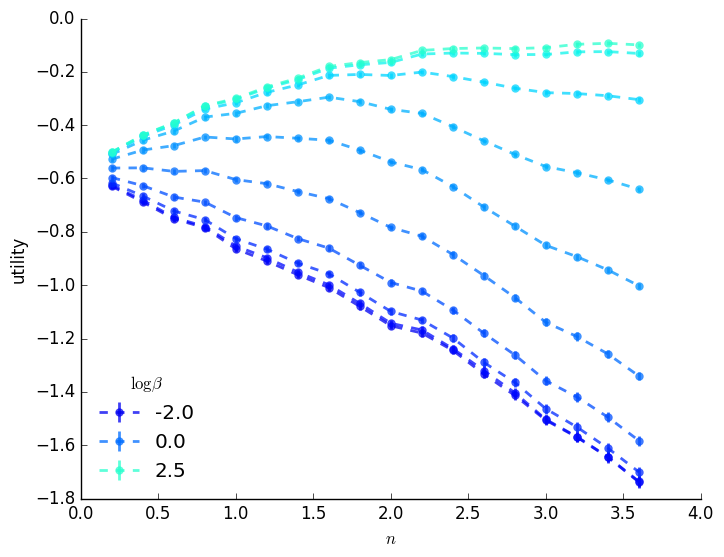
\includegraphics[width=0.45\textwidth]{figs_inef/utility.png}
  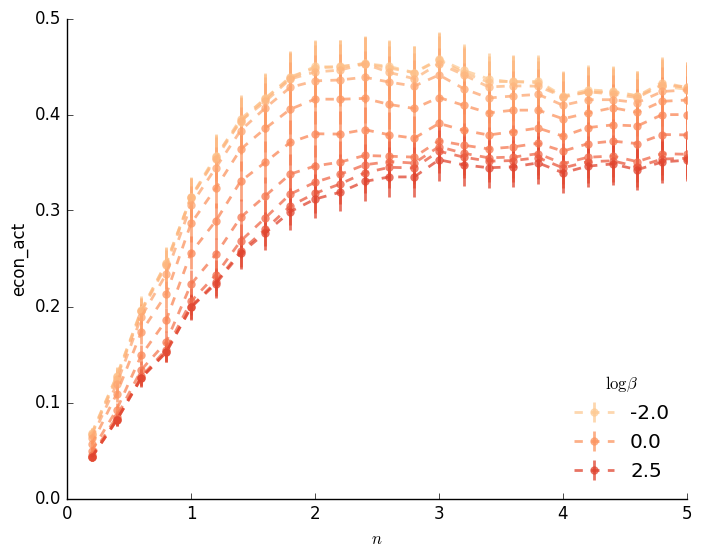
\includegraphics[width=0.45\textwidth]{figs_inef/econ_act.png}
  \caption{\textbf{(Left)} Average consumer utility per good as a function of the number of technologies per good $n$, for several degrees of inefficiency $\beta$ (when $\beta \to \infty$, the consumer strictly maximizes his utility). A large $n$ means there are more trades available for the consumer and a rational consumer should always increase his utility when faced with a growing number of possibilities. This is not the case for a consumer that chooses inefficiently. \textbf{(Right)} Average economic activity (volume of goods exchanged per good) as a function of $n$, for several degrees of inefficiency. An inefficient agent may choose poorly when faced with many choices, but he trades a larger quantity of goods.}
  \label{fig:intro_inef}
\end{figure}

We make the case that the best way to model a suboptimal utility choice is by removing the zero temperature limit, or $\beta \to \infty$, and adjust how much the consumer deviates from "rational" behavior by changing $\beta$. By lifting this simple restriction we  obtain nontrivial behavior, as shown on Figure \ref{fig:intro_inef}. On the left, we show the agents utility as a function of the number of technologies per good $n = N/ M$ for different values of $\log \beta$. When $\beta$ is large (around $10^2$), the agent optimizes efficiently enough that his utility always increases with $n$. However, when $\beta$ gets lower and the representative consumer starts making worse choices (according to his utility function), his expected utility in the market \textit{decreases} with $n$ instead of increasing.

This result corroborates an increasing number of empirical results from Behavioral Economics where the amount of choice a consumer faces may decrease the quality of his choices \cite{Lepper00, Schwartz02}. What is more interesting is that the economic activity in the market, in this case measured by the density of goods being exchanged, \textit{increases} with the inefficiency in consumer choice, because he deviates a lot more from $x_0$ than if he were strictly maximizing his utility. In this stylized economy, markets with agents that make bad decisions have unhappier agents but are more active and, considering economy activity is usually correlated with wealth, richer.

This work has been submitted as Jericó, J.P., Vicente, R. (2016) \emph{Information inefficiency in a random linear economy model}. Europhysics Letters



\subsection{Input-Output of random economies and real world data}

In Chapter \ref{cha:IO} we collect several years of the Input-Output tables for ten real world economies, which are matrices showing how much the industries of each sector of the economy produce and use as input of every good in the economy. The goods are also divided in the same sectors as the industries, in the case of the US at three levels of aggregation: detailed level, with 389 sectors, aggregated with 71 and summary with 15, going from "Mining" in the summary level to "Coal mining", "Iron, gold, silver mining", etc, in the detailed level, and at two levels of aggregation for the EU countries: 64 and 10 levels.

From these Input-Ouput tables we are able to build the Direct Requirement matrices, in which each element represents many dollars of a good are needed to produce a dollar of another good. These matrices represent directed, weighted graphs with the goods as nodes, and by definition the indegrees (sum of all edges that point to the node) are equal to one. The outdegrees, however, are variable, and they indicate the dependency of the production network on a specific good. Acemoglu et al \cite{Acemoglu12} show that the heavier tailed the outdegree distribution is, the more susceptible to shocks is an economy.

\begin{figure}[!ht]
  \centering
  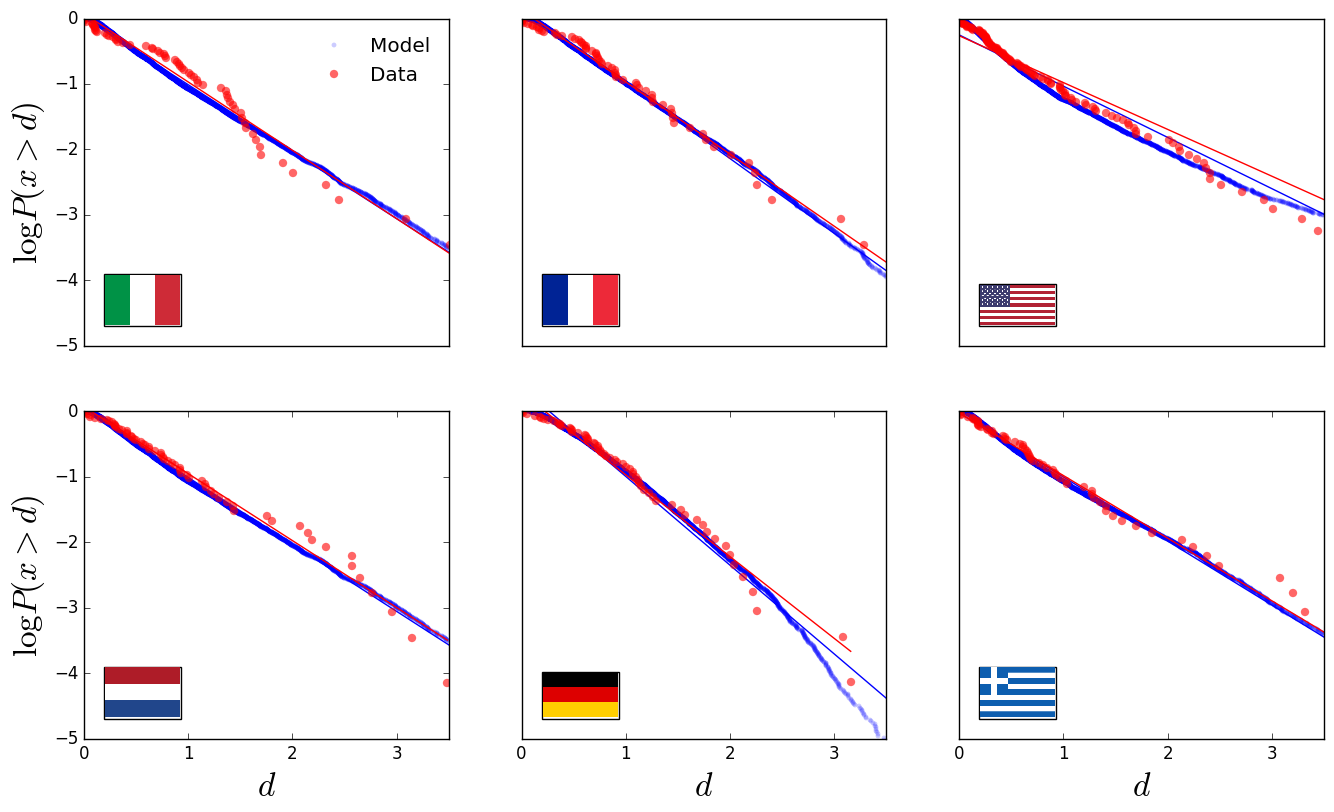
\includegraphics[width=0.95\textwidth]{figs_io/6panel_intro.png}
  \caption{Log of the counter cumulative degree distribution for six of the ten countries analyzed, compared with the closest degree distribution generated by the Random Linear Economy model with $M=100$, $\beta \to \infty$ for different values of $n$. Both datasets are plotted along with their regression, which is very close to an exponential distribution.}
  \label{fig:intro_io}
\end{figure}

We show that the outdegree (or simply degree) distribution of ten countries we have analysed at the aggregated level (64 sectors for the EU, 71 for the US) is very close to an exponential distribution, whereas data at the detailed level of aggregation for the US has much heavier tails. Given that these degrees are random variables with a fixed average, Information Theory tells us that in the absence of any extra constraints the distribution that maximizes entropy is an exponential distribution. This allows us to conjecture that the aggregation process has washed out the structural information of the economy.

We check this hypothesis by generating the Input-Output matrices, and consequently the Direct Requirement matrices, for artificial economies generated by the model introduced in Chapter \ref{cha:RLE} and showing that their aggregation produces the same patterns we observe in real world data. Furthermore, we show that different methods of aggregation yield different results, and the one employed in real world data is closer to random than to one that takes input and output correlations into account. This has a direct consequence on Acemoglu et al's conclusion for the structural fragility of the US economy: distribution tails that were taken into account may have been a simple artifact of the aggregation process, and the real distribution may be heavier tailed than what they calculated. If this is the case, the predictions made on \cite{Acemoglu12} concerning the fragility of the U.S. economy to random shocks may have been underestimated.

This work was accepted for publication as Jericó, J.P., Marsili, M. (2016) \emph{Input Output of random economies and real world data}. Eur. Phys. J. Special Topics: Can economics be a physical science?


\subsection{When does inequality freeze an economy?}

In Chapter \ref{cha:inequality} we show the statistical effects of inequality in a simple trading economy where we have $N$ agents with a initial capital that is power law distributed $P(c_i > c) \sim c^{-\beta}$, and agents trade $M$ goods each with its own price $\pi_1, \ldots, \pi_M$, such that the leftover cash of an agent is its capital $c_i$ minus the price of the goods he owns. At each trading step, one of the $M$ goods is chosen at random and its owner tries to sell it to another agent, which automatically accepts it if he has enough cash to do so.

The parameters are set in such a way that even the most expensive good is affordable to the poorest agent. Despite that, in the stationary state we show that this zero intelligence dynamic divides the agents into "classes" where an agent can afford goods up to a certain price and none more expensive than this threshold. If we define an agent's leftover cash as his liquidity in the market, given a unequal distribution of capital the economy's liquidity concentrates into fewer agents, and as the inequality parameter $\beta$ goes to one, the economy freezes completely as only the richest agents carry any meaningful trade.

\begin{figure}[!ht]
  \centering
  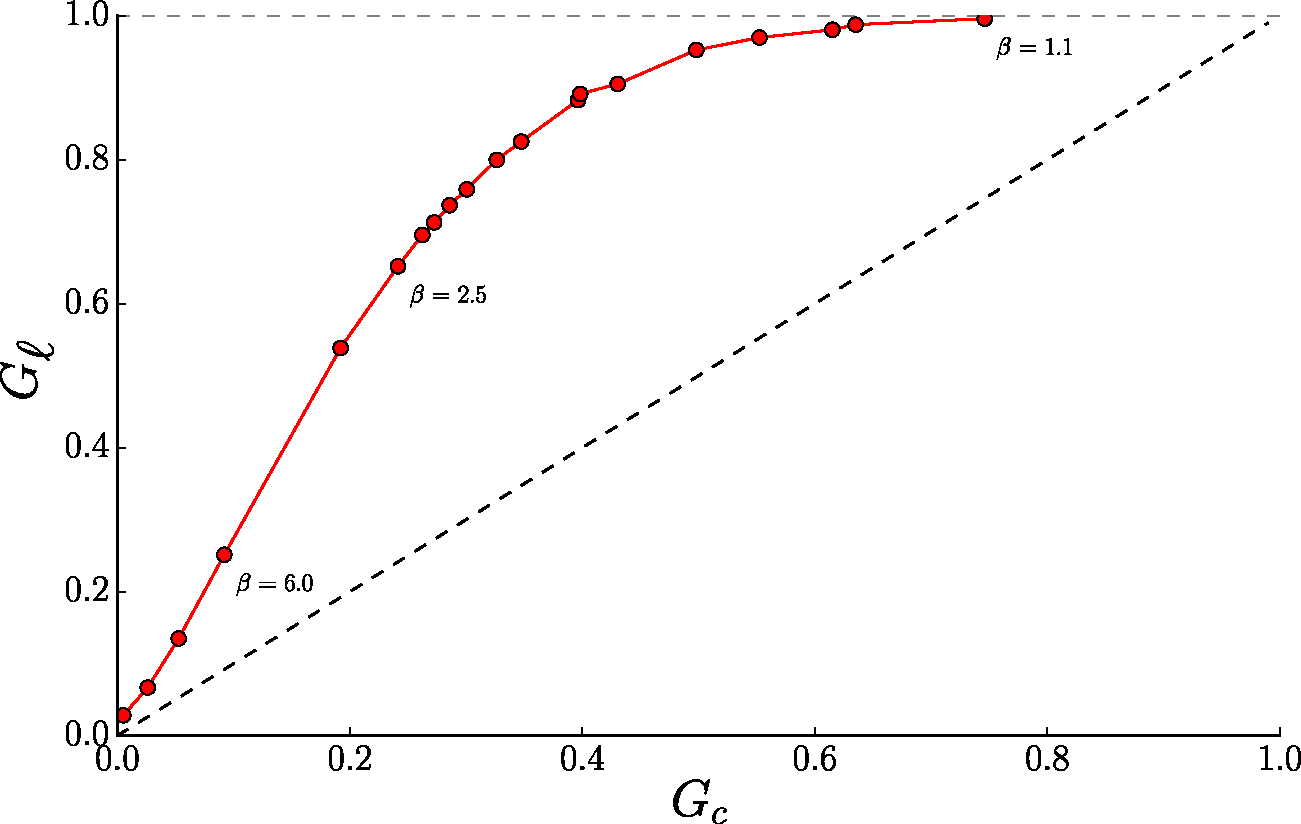
\includegraphics[width=0.65\textwidth]{figs_ineq/gini_intro.pdf}
  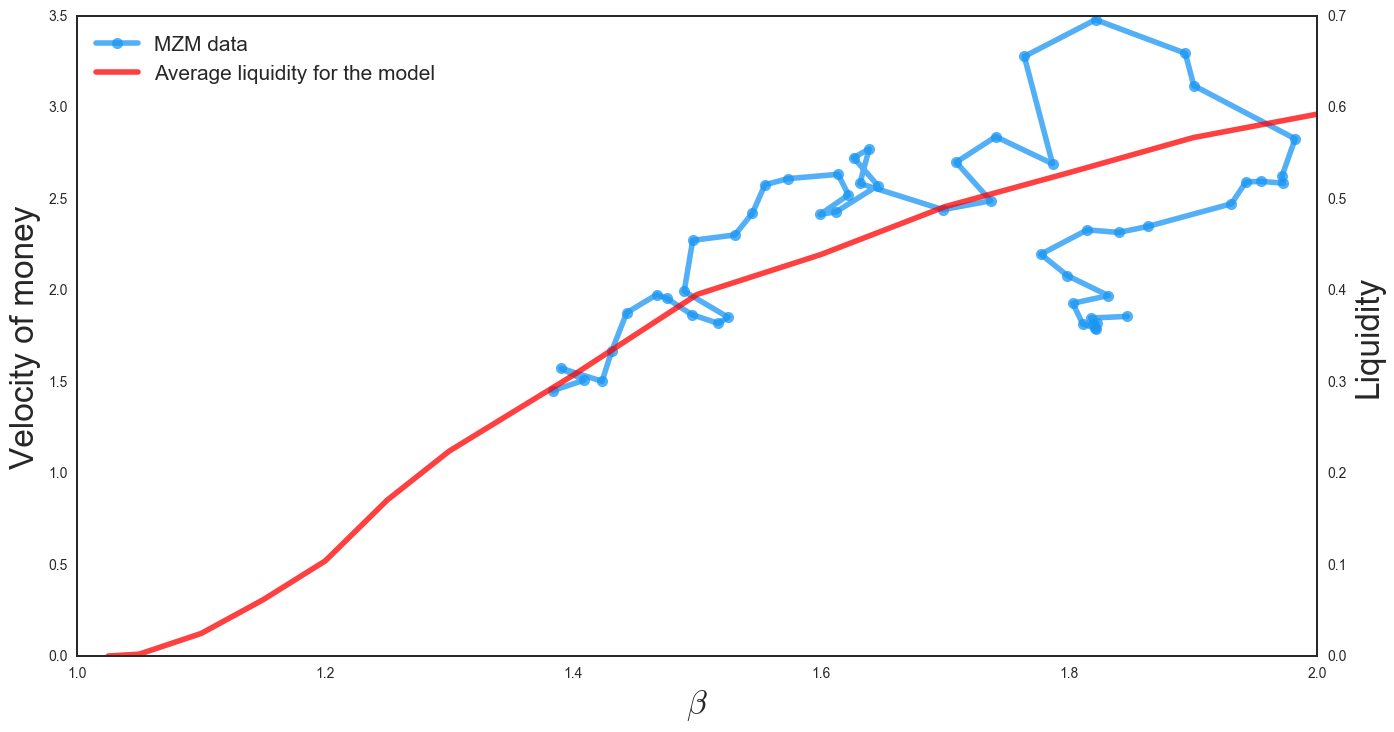
\includegraphics[width=0.65\textwidth]{figs_ineq/data_model.png}
  \caption{\textbf{(Top)} Gini coefficient $G_\ell$ of the cash distribution (liquid capital) in the stationary state as a function of the Gini $G_c$ of the capital distribution, for numerical simulations described in Chapter \ref{cha:inequality}. Cash, or liquidity, is always more unequally distributed than capital, resulting in perfect inequality (when only a countable number of agents have non zero liquidity) when $\beta$ approaches one. \textbf{(Bottom)} Velocity of money, defined for the model by equation \eqref{def:pavg}, as a function of the level of inequality represented by the power law parameter $\beta$, with comparison to the historical US data. Our model corroborates the fact that as inequality increases, the number of money units that are exchanged in a time interval decreases.}
  \label{fig:intro_ineq}
\end{figure}

These results are summed up by the top panel of Figure \ref{fig:intro_ineq}. There we plot the Gini coefficient for the cash as a function of the Gini coefficient for the capital. The Gini coefficient is a measure of inequality in a distribution and goes from zero to one: zero means perfect equality, all data in the dataset are the same. One means perfect inequality: only one point is positive and the rest is all zero. In Figure \ref{fig:intro_ineq}, we show that liquidity in the model is always much more concentrated than the initial capital, converging to perfect inequality when $\beta \to 1$. This has an arresting effect where all trade in the economy stops. This result is tested versus empirical data in the bottom panel of Figure \ref{fig:intro_ineq}, where we compare the velocity of money, as defined by the US Federal Reserver Bank, as a function of the inequality for the model and the historical US data, showing that there is good corroboration that inequality indeed decreases the velocity of money.


This work was published at Jericó, J.P., Landes, F. P., Marsili, M., Castillo, I.P. and Volpati, V. (2016) \emph{When does inequality freeze an economy?}. Journal of Statistical Mechanics: Theory and Experiment, Volume 2016.



\section{Organization of this thesis}

The first part of the thesis will concern the theoretical context of this work, along with some examples in the literature: in Chapter \ref{cha:GET} we will go over a brief introduction of General Equilibrium theory and mainstream Economics research in general. The main aim of the chapter is to give readers of a Physics background the necessary context to understand the standard protocol in Economics when studying a problem, what are some important questions in the field, what techniques are usually used, etc. Our goal is that after reading the chapter, the reader will be convinced of the proximity between the two fields, and how the methods differ despite their aims being essentially the same. 

In Chapter \ref{cha:stat_mech}, we will make the case of why Statistical Mechanics is a suitable tool for exploring and studying Economics. Although the Physics minded reader most likely does not need much convincing, it is still useful for those that never had any exposition to a general, information theoretical approach to Statistical Mechanics as introduced by Jaynes \cite{Jaynes57}. We hope that a reader with a background in Economics (and who hopefully did not stop reading the thesis after Chapter \ref{cha:GET}) will agree with us that the methods presented therein offer an alternative to the usual methods in Economics. In this chapter we will also present a number of previous work that have already explored this intersection.

We end the first part by introducing the Random Linear Economy model in Chapter \ref{cha:RLE}, which consists of a simple market model where companies have random technologies and one consumer wishes to improve his utility by trading his current goods in the market, which is exactly the sort of problem General Equilibrium Theory describes. Despite its simplicity, the model exhibits a rich behavior due to the stochasticity introduced in the technologies and its solution is arrived at by using techniques from the Physics of disordered systems. Its introduction merits a dedicated chapter because not only it serves as the basis for the work developed on Chapter \ref{cha:inefficient} and parts of Chapter \ref{cha:IO}, but also because it is a good representative of the ideas put forward in Chapters \ref{cha:GET} and \ref{cha:stat_mech}.

The second part of this thesis, Chapters \ref{cha:inefficient}, \ref{cha:IO} and \ref{cha:inequality}, are the three problems we have mentioned in the last section. 


\part{Theory}

\chapter{Economics and the General Equilibrium Theory}

In this chapter we will discuss some of the economic theories behind
the work of the thesis. Mainly, we will introduce General Equilibrium
Theory and some of its main results and statements. We will then
discuss how it relates to Statistical Physics and some of its
criticism in the Economics literature.

General Equilibrium Theory is a mature and consolidated field of
Economics \cite{Arrow54, mascolell, mckenzie} which aims to
characterize the existence and properties of equilibria in certain
market settings. Economic systems are assumed to frequently have
actors with opposing goals: the owner of a good wants to sell it for
the highest possible price, while its potential buyers would like to
purchase it for as low as possible. Fishermen would like to catch as
many fishes as possible as long as their peers care to not also overdo
it otherwise they may extinguish the oceans. In this way, one expects
economies and markets to converge to a certain steady state and among
other things, General Equilibrium Theory characterizes these steady
states in a rigorous manner. In this sense, it's also a theory in
Microeconomic, because it explains macrobehavior from the incentives
of microscopic agents.

While the work in this thesis does not aim to strictly expand
economies as they are describe in General Equilibrium Theory, it's
purposes and questions are very similar to the ones physicists usually
go for when studying an economic system: namely, the characterization
of it's equilibrium state. It's important, therefore, to have a
deeper understanding of how it's done in economics, what are the main
concerns and assumptions.

\section{A Brief Exposition}

The exposition in this chapter is mostly adapted and simplified from
\cite{mascolell} and will be considerably more formal than the rest of
this thesis. This is due to the way the discipline is commonly
studied.

In General Equilibrium Theory, an economy is defined through the
following components: we assume $J$ consumers, $N$ firms and $M$
goods. Each consumer has a consumption set $X_j$ which contains all
possible consumption bundles $x_j = (x_j^1, \ldots x_j^M)$ that the
consumer has access to, ie, each bundle $x_j$ is a $M-$dimensional
vector with nonnegative entries (we are assuming he cannot consume a
negative amount of a good). $X_j$ is limited by ``physical''
contraints, such as no access to water or bread, but not monetary
constraints, which will arise later.

The consumer also has an utility function $U_j(x)$ that takes every
element $x_j \in X_j$ to a real number, representing how much the
consumer values each bundle of his consumption set. This allows us to
define define a preference relationship over the elements in $X_j$
(ie, if the consumer prefers bundle $x$ to $x'$), which is
\textbf{complete}\footnote{For every $x, x' \in X_j$, either
  $U_j(x) \geq U_j(x')$ or $U_j(x) \leq U_j(x')$.} and
\textbf{transitive}\footnote{For every $x, y, z \in X_j$, if
  $U_j(x) \geq U_j(y)$ and $U_j(y) \geq U_j(z)$, then
  $U_j(x) \geq U_j(z)$.}, two standard requirements in Economics for
rational behavior.

Finally, the consumer is also endowed with an initial bundle of goods
$\omega_j = (\omega_j^1, \ldots, \omega_j^M)$, $\omega_j^\mu \geq 0$
which will define his budget given a set of prices for the goods and
will constraint his choices on $X_j$.

Each firm $i$ has a production set $\Xi_i$ of technologies
$\xi_i = (\xi_i^1, \ldots, \xi_i^M)$ which it is able to operate. Unlike
consumption bundles, which are final allocations and therefore must be
nonnegative, technologies can be any real number: the negative entries
are inputs and the positive entries are outputs that the firm can
operate. $\Xi_i$ is also limited only by ``physical'' constraints, not
by monetary constraints. A firm that has $\xi_i = (-1, 2)$ in its
production set is able to transform one unit of good 1 into two units
of good 2. It won't necessarily be able to transform two units of good
1 into four units of good 2, for that it must also have $\xi'_i = (-2,
4)$ in $\Xi_i$. It might be the case, for example, that companies get more efficient
with production and therefore it might have $\xi''_i = (-2, 6)$ in its
production set.

In General Equilibrium Theory, an economy is formally defined as the tuple

\begin{equation}
  E = \left(\{(X_j,U_j)\}_{j=1}^J,
    \{\Xi_i\}_{i=1}^N, \{\omega_j\}_{j=1}^J \right).\label{eq:econGE}
\end{equation}

One of the theory's assumptions is that the economy described is
\textbf{complete}, that is, every agent can exchange every good with no
transaction costs and complete information about the firm's
technologies, other consumer's consumption, etc. Also, a good $\mu$
contains all the possible information that a consumer would take into
account when making his choice. That is, among the space of goods we
could have ``umbrella'' and ``chocolate'', or we could also have ``an
umbrella on August 13th, 2016 in Sao Paulo with 50\% chance of rain''
and ``an umbrella on December 12th, 2016 in Chicago with 90\% chance
of rain''. 

It's assumed that agents are \textbf{price-takers}, that is, they are
unable to affect the market prices and therefore take them as a
given. The prices of the goods are given by a $M-$dimensional vector
$p = (p_1, \ldots, p_M)$, where each price is a strictly positive
quantity, ie, $p_\mu>0$ for all $\mu$. This assumes that goods have global
prices, which is consistent with the completeness assumption: there is
no reason why the market prices should be different for certain
consumers or firms if they have complete knowledge and no transaction
costs.

With a price vector $p$ defined, we say the consumer $j$ has a budget
$B_j = p\cdot \omega_j$, which is the monetary value of his initial
endowment. Any bundle he chooses to purchase will cost him
$p\cdot x_j$. His objective, therefore, is to find the best bundle
$x_j$ he is able to afford, that is:

\begin{equation}
  \label{eq:consumer_obj}
  \max_{x_j \in X_j} U(x_j), \quad \text{s.t. } p\cdot x_j \leq p\cdot \omega_j
\end{equation}

The firms, on the other hand, have an operating profit for each
technology given by $p \cdot \xi_i$, which is how much money they earn
by selling their outputs ($\xi_i^\mu > 0$) minus how much they spend
purchasing the inputs ($\xi_i^\mu < 0$). Their objective is to maximize
their profits, that is:

\begin{equation}
  \label{eq:firm_obj}
  \max_{\xi_i \in \Xi_i} p \cdot \xi_i
\end{equation}

With these ingredients laid out, we define an \textbf{allocation} of the
economy as a set of specific choices for consumption bundles and
technologies, ie, an allocation $a$ of an economy $E$ is

\begin{equation}
  \label{eq:3}
  a = (x_1, \ldots, x_J, \xi_1, \ldots, \xi_N), \, x_j \in X_j, \,
  \xi_i \in \Xi_i
\end{equation}

The economy is closed, and therefore all that is produced must come
from the initial endowments and be consumed by the consumers. We
therefore say an allocation is \textbf{feasible} if it satisfies
\textbf{market clearing} for all the goods:

\begin{equation}
  \label{eq:market_clearing}
  \sum_{j=1}^J x^\mu_j = \sum_{j=1}^J \omega_j^\mu + \sum_{i=1}^N
  \xi_i^\mu, \quad \forall \, \mu \in \{1,\ldots, M\}
\end{equation}

This is a strong condition which constraints many quantities in
the economy. In particular, if we multiply both sides of the equation
by $p^\mu$ and sum then in $\mu$ we get, in vector notation,

\begin{equation}
  \label{eq:price_market_clearing}
  \sum_{j = 1}^J p \cdot (x_j - \omega_j) = \sum_{i=1}^N p\cdot \xi_i
\end{equation}

The left handside is the leftover money the consumers have after
making their choice of consumption, also called the value of excess
demand, whereas the right handside is the firms aggregate profit, also
known as the value of excess suply. Because we assume that the
consumer may not spend more than his budget, the value of each
consumer's individual excess demand has to be non
positive. Simultaneously, if we assume that the firms always have
$\xi_i = 0$ in their production set, ie, we assume that they can
always opt to not produce at all and leave the market, then the value
of excess supply for each firm has to be non negative. Because they
must be equal, we conclude that in an economy for which market
clearing holds, the consumer spends all his available budget and the
firms all have zero profit, a result known as \textbf{Walras' Law}.

Given a set of possible feasible allocations $\{a_k\}$, we may wonder
if there is any allocation we desire most over the other. This
of course depends on the criteria we use to judge them: we may like
allocations with less inequality, with the most aggregate utility,
with the smallest minimum utility, etc. Economist opt to use one
particular condition which is called \textbf{Pareto optmality}.

Intuitively, a \textbf{Pareto optimal} (or \textbf{Pareto efficient}
allocation is one that you can't make a consumer better without making
another consumer worse off. The idea is that, a non Pareto optimal
allocation has some waste in it: one could change the consumption
bundles in order to increase some utilities and no other consumer
would complain. Because firms have zero profit in feasible
allocations, they wouldn't mind the change. 

More formally, a feasible allocation $a = (x, \xi)$ is said to be
\textbf{Pareto optimal} if there is no other allocation that
\textbf{Pareto dominates} it, that is, no allocation $a' = (x', \xi')$
such that $U(x_j') \geq U(x_j)$ for all $j$ and $U(x_j') > U(x_j)$ for
at least one $j$.

The Pareto optimality concept therefore defines a socially desireble
outcome in a ``non-controversial'' way, by definition no agent in the
economy would have a problem with policies or actions taken to make it
more Pareto efficient. However, it says nothing about equality: an
allocation in which one consumer has all the goods and no other
consumer has any goods is Pareto optimal.

We finally arrive to the concept of equilibrium in an economy. A
\textbf{Walrasian equilibrium} (or competitive equilibrium or simply
equilibrium) in an economy E is an allocation $(x^\ast, \xi^\ast)$ and a
price vector $p$ such that

\begin{enumerate}
\item Every firm $i$ maximizes it's profits in its production set
  $\Xi_i$, that is
  \begin{equation}
    \label{eq:4}
    p\cdot \xi_i^\ast \geq p\cdot \xi_i, \quad \forall \xi_i \in
    \Xi_i,\quad \forall i in \{1, \ldots, N\} 
  \end{equation}
\item Every consumer $j$ maximizes his utility in his consumption set
  $X_j$, that is
  \begin{equation}
    \label{eq:1}
    U(x_j^\ast) \geq U(x_j), \quad \forall x_j \in X_j, \quad \forall
    j \in \{1,\ldots, J\}
  \end{equation}
\item The allocation $(x^\ast, \xi^\ast)$ is feasible, that is,
  \begin{equation}
    \label{eq:2}
    \sum_{i=j}^J x_j^\ast = \sum_{j=1}^J \omega_j + \sum_{i=1}^N \xi_i^\ast
  \end{equation}
\end{enumerate}

The Walrasian equilibrium is essentially a pair allocation - prices in
each all the optimization problems are solved at once. Although we
have made no mention of dynamics in this economy, it's considered an
equilibrium because all agents are as satisfied as possible with their
allocation given the prices, which we have assumed to be global and
unchangeable by any agent's action. This is not exactly a definition
of equilibrium as used in Physics, but we will discuss this point
later. For now, we point out that a Walrasian equilibrium is in some
sense stable.

One 

We have thus defined two desirable properties of an allocation:
efficiency and equilibrium. The fundamental results of General
Equilibrium Theory are the \textbf{welfare theorems}, which define the
conditions in which an equilibrium is Pareto optimal and vice versa.

The \textbf{First Fundamental Welfare Theorem} asserts that if the consumers have
a utility function continuous on $X_j$\footnote{The actual theorem
  asserts a weaker condition, that the preferences be locally
  nonsatiated, that is, for every $x \in X$, there is an $x' \in X$
  such that $\|x - x'\| < \varepsilon$ and $x'$ is preferred to $x$.},
then all Walrasian equilibria are Pareto optimal. This result is
simple yet useful, because it tells us that if our economy is in
equilibrium, we don't have to care about checking if it's
efficient. The violation is also important: if a given economy we are
studying is in an inefficient equilibrium, then it must be that one of
the theorem's condition was violated. This sheds light in where to
look for market failures. We remind the reader, however, that some
extra strong assumptions were made for the economies described by this
therorem, namely, completeness of market and global prices that
no single agent is capable of influencing.

The \textbf{Second Fundamental Welfare Theorem} requires extra
assumptions: it afirms that if an economy satisfies the condition of
the first fundamental theorem, the utility functions $U_j$ plus all
sets $X_j$ and $Y_i$ are convex and if we are able to redistribute the
initial endowments at will while keeping the total amount
$\sum_{j=1}^J \omega_j$ constant, then for every Pareto efficient
allocation there exists a wealth allocation $\omega$ and price vector
$p^\ast$ such that $(x^\ast, \xi^\ast, p^\ast)$ is a Walrasian
equilibrium.

The second theorem is considerably more interesting than the first
one: any Pareto optimal allocation we would like in an economy can be
an equilibrium given the appropriate price vector and a possible
wealth transfer, albeit under a stronger set of conditions.

\section{The Dynamics of General Equilibrium}

A conspicuous element was missing from the exposition above: there are
no rules for the dynamics of the economies described above. The prices
are taken as a given, as are the consumer and firm choices. What
happens if a firm closes? What happens if a new firm appears? The
equilibrium simply ``recalculates'' and the economy moves to the new one?

Indeed, this is a long standing criticism of General Equilibrium
Theory. Walras proposed it as a process of
\textbf{tatônnement}\footnote{From ``trial and error'' in french}: a
central figure, known as the Walrasian auctioneer, sugests a price and
asks all the firms and consumers how much would they like to produce
and buy at these given prices, but without any transaction taking
place at the out of equilibrium prices. The auctioneer updates the
prices in the direction of diminishing excess demand or supply, a
``gradient descent'' of sorts, until equilibrium is reached.

However, this process is quite indetermined. Chiefly, this auctioneer
figure doesn't exist in most decentralized markets: goods are traded
at agreed prices by both parts, which do not wait until their
transaction is authorized by some central authority. Even if they did,
such an auctioneer would require an infinitely large computational
capability to compute the excess demand and supply of every consumer
and firm and for every good in a modern economy \cite{axtell05,
  Roughgarden10}. Worst of all, even if there was such central figure
with such an arbitrary large amount of computing power, the price
updating dynamic is not guaranteed to
converge \cite{Gintis07}. Finally, even if it converges, we have no
assurance that it will converge in finite time.




%computable general equilibrium

% general equilibrium theory
% def of walrasian eq, market clearing, welfare theorems
% criticisms
% diff between economic equilibria and physics equilibria
\cite{thurner} \cite{Schumpeter39} \cite{savage} \cite{mascolell}

\cite{Tversky74, Kahneman79, Tversky81}


\chapter{Statistical Mechanics and Inference}
\label{cha:stat_mech}
In this Chapter we aim at answering the question of why Statistical Mechanics is suitable to study economic systems. The essence of the answer is that, among other things, the techniques of Physics allows one to find the minimum energy configuration (or at least very good approximations) and the expectation value of certain quantities of interest in rather complicated settings, which is precisely what Economics could mostly benefit of. 

To the reader familiar with Statistical Mechanics, we draw attention to the fact that we present here the canonical ensemble not as a derivation from Thermodynamics, but as a systematic inference of a system's observables using Information Theory. Instead of assuming a system connected to a heat bath at a fixed temperature and employing the first postulate of Statistical Physics, we follow the work of Jaynes \cite{Jaynes57} and show that the Gibbs distribution is the solution for an inference problem with limited information.

\section{Statistical Mechanics as an inference problem}

Suppose we have an interacting system composed of $N$ particles, each with its own state $x_i$, which can be its position, velocity, orientation, decision of whether to buy a Mac or a PC, political affiliation, etc. The whole system can be fully characterized by the configuration vector $x = (x_1, \ldots, x_N)$ and we assume all the information we have about this system is the expected value of function $H(x)$, often called in physics settings the energy function. There are many questions we can ask about the system, for example what is the probability of this system being at a configuration $x$, or what is the expected value of another quantity $G(x)$. These questions are inference problems, and through Information Theory we can find out what is the best way we can answer them.

As proposed by Shannon \cite{shannon1948}, when faced with a choice of several probability functions that describe some data or phenomena, one should always opt for that which makes the least assumptions, given the constraints of the problem. This amounts to finding the probability distribution $p(x)$ that maximizes the \textbf{Shannon entropy}

%TODO: show the shannon entropy in an Appendix maybe?
\begin{equation}
    S[p] = - \int dx P(x) \log P(x)
\end{equation}
subject to the constraints imposed by observation. In our case, the constraint is that the energy function $H(x)$ has an average value $\langle H(x) \rangle = \int dx \, P(x) H(x) = E$ and we also have to impose the constraint that $P(x)$ is a probability distribution and therefore must be normalized, i.e., $\int dx \, P(x) = 1$. This means that to find $P(x)$ for our system, we must find $P(x)$ that maximizes the Lagrangian

\begin{equation}
\mathcal{L}[P] =  - \int dx P(x) \log P(x) + \alpha \left(\int dx \, P(x) - 1\right) + \beta \left( \int dx \, P(x) H(x) - E \right),
\end{equation}
where $\alpha$ and $\beta$ are the Lagrange multipliers of this maximization problem. 

We assume that at the maximum $P^\ast$ a small perturbation $P(x) + \delta P(x)$ does not alter the Shannon entropy. If we assume that all $\delta P(x)$ are independent (i.e., $\delta P(x)$ and $\delta P(x')$ are not correlated for every $x, x'$ in the support of the distribution), then for every $x$ this becomes a regular maximization problem. For every $x$, we must solve that $\frac{\delta \mathcal{L}(P)}{\delta P} (x)$ is equal to zero, that is:

\begin{equation}
\frac{\partial}{\partial P(x)}\left\{ -P(x) \log P(x) + \alpha \left(P(x) - 1\right) - \beta \left(P(x) H(x) - E\right) \right\} = 0, \quad \forall x  
\end{equation}

Solving this equation we have that for every value of $x$

\begin{align}
    & -\log P(x) - 1 + \alpha + \beta H(x) = 0 \Rightarrow \\
    & \Rightarrow  P(x) = e^{-1 + \alpha - \beta H(x)}
\end{align}

The Lagrange multipliers must be set so that the constraints are satisfied. For $\alpha$ we have that $e^{\alpha - 1}$ must normalize the probability distribution, i.e.

\begin{align}
   &  \int dx e^{-1 + \alpha - \beta H(x)} = 1 \Rightarrow \\
    & e^{1 - \alpha} = \int dx e^{- \beta H(x)} = Z
\end{align}

This normalization term is the sum over all the configurations and is called the \textbf{partition function}. For $\beta$ we must have that 

\begin{equation}
    \int dx H(x) \frac{e^{-\beta H(x)}}{Z} = - \frac{\partial}{\partial \beta} \log Z = E
\end{equation}

This means $\beta$ must be such that the average energy of the system is equal to the observed average $E$. However, suppose we have not actually observed $E$, all we know is that it is fixed to some  value. Then, because $E$ is given by the above equation for which the only degree of freedom is a Lagrange multiplier, all the possible values it can take are given by varying $\beta$ from 0 to $\infty$. We have finally arrived at the maximum entropy distribution for our inference problem, which is the \textbf{Gibbs distribution}

\begin{equation}
\label{eq:sm_gibbs}
    P (x | \beta) = \frac{1}{Z(\beta)} e^{-\beta H(x)}
\end{equation}

The extreme cases for $\beta$ give us an intuition on how the Gibbs distribution behaves. For $\beta = 0$, $P(x) = \frac{1}{Z}$, for all values of $x$: in this limit all configurations are equally likely, regardless of their energy $H(x)$. In the opposite case, when $\beta \to \infty$, $Z$ becomes more and more concentrated around its maximum point, where $E(x)$ is minimum, and eventually $P(x)$ collapses to a delta function around the minimum energy configuration, also known as the \textbf{ground state} (it can also have an equal mass in several points in the case of multiple minima). Therefore, in the full $\beta$ spectrum, the Gibbs distribution starts completely uniform in the space of all configurations and slowly coalesces around the minimum energy values. If we assume $H(x)$ is bounded, then for every finite value of $\beta$, the system has a finite probability of being in any configuration (what is known as ergodicity). Given a system described by the Gibbs distribution, the average value of another desired observable $G(x)$ is given by

\begin{equation}
g = \langle G(x) \rangle = \int dx G(X) \frac{1}{Z} e^{-\beta H(x)}
\end{equation}

Though we have called $H(x)$ the energy function for customary reasons, this function is in principle any arbitrary function of the system configuration that has a well defined average value. For most systems of interest we can always decompose it as a sum of small scale interactions, that is, we can write

\begin{equation}
    H(x) = \sum_{a} H_a (x_a),
\end{equation}
where $a$ represent minimal cliques, usually pairwise, where we can reduce the interactions in the system to microscopic interactions. In this way, the behavior of macroscopic quantities such as the average energy or any other observable we are interested depends on the sum of a large amount of simple interactions. 

Besides allowing for more realistic modelling, interactions have a side effect which is very well known to physicists but that don't appear frequently in economic debates: the existence of \textbf{phase transitions}. Instead of asking questions about the specific details of one equilibrium configuration, in Physics one usually explore the parameter space looking for sharp transitions in the behavior of average quantities such as average utility per agent, average number of goods traded, etc. Phase transitions are of special interest because they represent some of the most interesting phenomena a system can present, and indeed, many popular questions in Economics, such as business cycles, crisis, altruistic cooperation, etc, can be framed in terms of phase transitions.

We note that despite this being the standard theory for the canonical ensemble in Statistical Physics, we have not made so far any Thermodynamical (or any other "physical") assumptions. We have been describing generic systems where we simply applied the tools of Information Theory for the inference of a random variable for which we have limited information. There's nothing that limits us to using the Gibbs distribution only for gases in which the molecules interact according to the laws of Physics. This is the fundamental reason why Statistical Mechanics is so successful at explaining such a varied wealth of phenomena: despite being first developed via physical laws, its results are general.

The only real difference when dealing with a thermodynamical system is that when we plug the Gibbs equation back into the Shannon entropy we have

\begin{equation}
    S[P_G] = \log Z + \beta E,
\end{equation}
which is still general, but we can now use one of the Maxwell's relations to give $\beta$ a physical interpretation:

\begin{equation}
   \frac{1}{T} = \frac{\partial S}{\partial E} = \beta
\end{equation}

Therefore in physical systems $\beta$ is identified as the inverse temperature and when $T \to \infty$, the system is equally likely to assume any possible configuration. Likewise, when $T = 0$, the system is frozen at one of the ground states. 


\subsection{A simple example}

We make explicit the general nature of the Gibbs distribution deduced in this section by a simple example\footnote{This example was taken from the course notes of Nestor Caticha.} of a random variable $x$ that can take three values: -1, 0 or 1. We know it's average is $\langle x \rangle = m$. What is the best inference we can make for it's probability distribution $P(x)$? The Gibbs distribution is

\begin{equation}
   P(x) = \frac{e^{-\lambda x}}{Z(\lambda)},
\end{equation}
where $Z(\lambda)$ is given by:

\begin{equation}
   Z(\lambda) = \sum_{x\in \{-1, 0, 1\}} e^{-\lambda x} =
   1 + 2\cosh \lambda
\end{equation}

And $\lambda$ is given by

\begin{equation}
   m = - \frac{\partial}{\partial \lambda} \log Z(\lambda) =  - \frac{2 \sinh \lambda}{1 + 2 \cosh \lambda}
\end{equation}

Writing $u = e^{-\lambda}$ and writing the hyperbolic functions as $2 \cosh \lambda = e^\lambda + e^{-\lambda}$ and $2 \sinh \lambda = e^\lambda - e^{-\lambda}$ we have

\begin{equation}
   \frac{u - u^{-1}}{1 + u + u^{-1}} = m \Rightarrow 
   m + (m+1)u + (m -1) u^{-1} = 0
\end{equation}

Multiplying both sides of the equation by $u$, we have the second order equation $(m - 1) u^2 + m u + (m + 1) = 0$, for which the (positive) solution is

\begin{equation}
   u = \frac{-m - \sqrt{m^2 - 4(m^2 - 1)}}{2 (m - 1)}
\end{equation}

\begin{figure}[!ht]
  \centering
  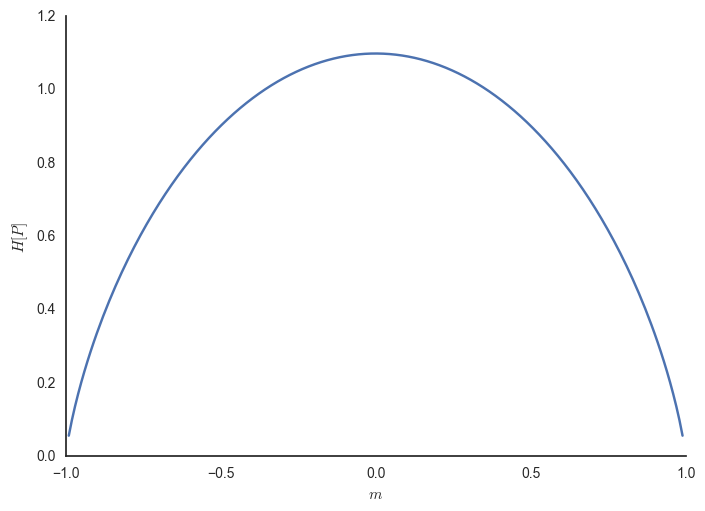
\includegraphics[width=0.4\textwidth]{figs_statmech/fig1a.png}
  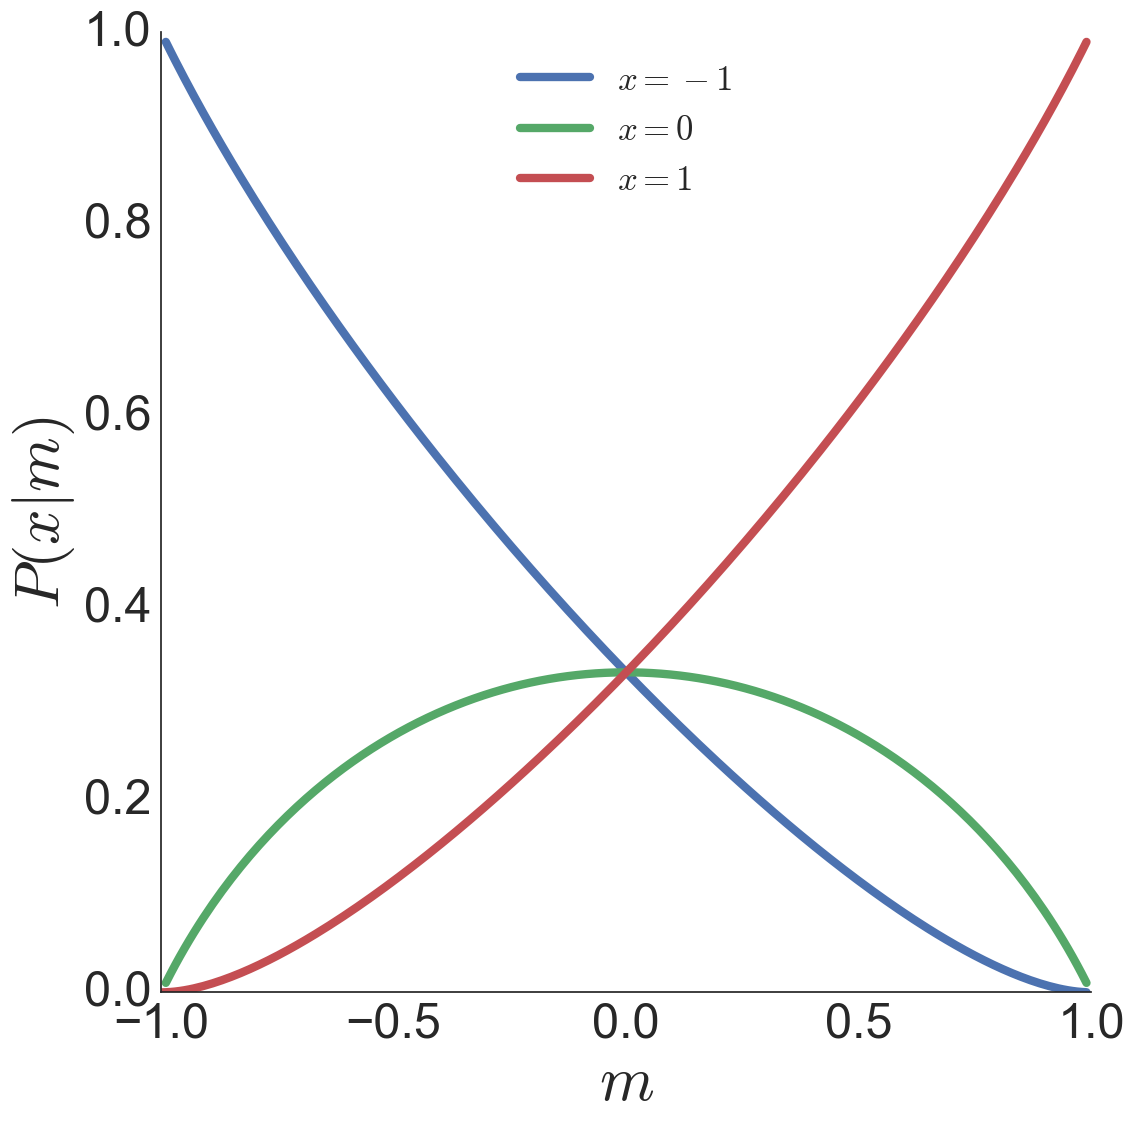
\includegraphics[width=0.4\textwidth]{figs_statmech/fig1b.png}
  \caption{\textbf{(Left)} Entropy $H[P]$ for the Gibbs distribution of a random variable $x$ that takes three values, -1, 0 and 1 as a function of its known average $\langle x \rangle = m$. \textbf{(Right)} Probability distribution $P_G(x|m)$ as a function of $m$ for each of the three values.}
  \label{fig:simple_example}
\end{figure}

And finally we find that $\lambda = -\log u$. We plot on Figure \ref{fig:simple_example} the entropy for the Gibbs distribution as a function of $m$ and the probability $P(x|m)$ for the three values. We see that as expected entropy is maximal when the three states are equally likely, and when $m = \pm 1$ the variable is fully identified, so the entropy goes to zero.


\subsection{Optimization Problems}

The Gibbs distribution offers a natural way of solving maximization problems: given a system that we know has energy function $H(x)$, its ground state is simply the distribution of states $x$ at zero temperature, or at $\beta \to \infty$. Likewise, we can find any quantity of interest $G(x)$ at the maximum by computing $\langle G(x) \rangle$ in that limit. 

This is certainly not the only way one can find solutions to optimization problems, however, framing it as a Statistical Physics problem has a couple of benefits, namely, if we accept approximate solutions, we can find them very close to the optimal in a time orders of magnitude smaller. Usually this is done using general purpose Monte Carlo algorithms to sample from the Gibbs distribution at a certain $\beta$ value and slowly increasing $\beta$ up (i.e., decreasing the system's temperature) until convergence, a technique known as \textbf{simulated annealing}. For well behaved convex functions there are certainly more efficient optimization algorithms, but Monte Carlo techniques are very robust and allow us to add constraints and interactions in the energy function without having to adopt an alternative maximization procedure.

As an example from \cite{mezard2004}, consider a conference planner that would like to distribute $N$ scientists in two available hotels. Scientists either like or dislike each other. We represent this by a positive interaction constant $J_{ij} = 1$ if $i$ and $j$ like each other and $J_{ij} = -1$ if $i$ and $j$ don't like each other. Scientists would then prefer to stay in hotels with their friends and not be in the same hotel with scientists they don't like. If we represent the hotel that a scientist is by $s_i = \pm 1$, the planner has to optimize for each scientist $i$ his utility

\begin{equation}
   u_i (\vec{s}) = \sum_{j=1, j\neq i}^N J_{ij} s_i s_j
\end{equation}

And then his problem is to find the configuration $\vec{s}$ which maximizes the total utility for all scientists, i.e.

\begin{equation}
   U(\vec{s}) = \sum_{i} u_i(\vec{s}) = \sum_{i, j} J_{ij} s_i s_j.
\end{equation}

For as little as 3 scientists, the problem can be frustrated: if all $J_{ij} = -1$ or if two are positive and one is negative, there are multiple ground states. For the general case, a brute force solution would require a search over $2^N$ configurations, which is unfeasible even for conferences with $N=100$ participants. However, with a Monte Carlo simulation we can find close approximations much more quickly.

This scenario, of course, is the Sherrington-Kirkpatrick model of a simple \textbf{spin glass}. Indeed, the theory of spin glasses are a very successful case in which complex systems with non regular patterns of interaction (also called \textbf{disordered systems}) can be studied, often solved analytically and exhibit very rich and interesting behavior.

These scenarios are not limited to physical systems: in portfolio optimization theory, one usually assumes that given a pool of possible financial assets, each with expected return $R_i$ and a covariance matrix $C$ for all assets, then given a fixed total assumed risk there is only one portfolio composition that maximizes the return and that a rational agent should adopt \cite{elton2009}. However, if one adds in the portfolio composition problem the requirement that any buy or sell operation carries a fee proportional to the value of the asset, then the optimization problem becomes glassy, presenting an exponential number of solutions to the number of available assets \cite{galluccio1998, gabor1999}. These aren't suboptimal solutions due to high temperature, but optimal portfolios a perfectly rational agent would choose.


\section{In Economics}

The utility of employing Statistical Mechanics to better model economic problems has not gone unnoticed by economists, even though it's usage is far from mainstream. It is most frequently used in interaction based models, in areas such as Game Theory, which arose precisely to deal with situations in which the decision of one agent affects the payoff of another, and rising microeconomic fields such as Social Interactions \cite{ScheinkmanSocialInt}. 

Probably the most influential work to show how a large interacting population can lead to unexpected outcomes is Schelling work on segregation \cite{schelling1971}, where two types of agents live in a city and all agents prefer to live in neighborhoods where their type is slightly more common than the other. This search for optimality will lead to complete segregation of agents, despite everyone preferring to live in mixed areas. In Schelling's words: "there is no simple correspondence of individual incentive to collective results". For a Statistical Mechanics treatment of Schelling's segregation model, we refer the reader to \cite{dall2008}.

One of the first major proposals of connecting Statistical Mechanics with Economics came from Santa Fe Institute's seminal work \textit{The economy as an evolving complex system} \cite{Anderson88, Arthur97}, which influenced physicists and economists alike. 

Later, in \cite{brock2001a} and \cite{brock2001b}, Brock and Durlauf describe an interacting model where each agent $i$ chooses between two binary actions $\omega_i = -1$ or $\omega_i = 1$ and his utility function has three terms: a private, deterministic term $u(\omega_i)$, one that interacts with other agents via a $J\omega_i \omega_j$ utility interaction and a random shock $\epsilon(\omega_i)$ whose distribution is given by the probability that $\epsilon(\omega_i = 1)$ is larger than $\epsilon(\omega_i = -1)$, given by a logistic distribution

\begin{equation}
P(\epsilon(1) - \epsilon(-1) > x) = \frac{1}{1 + e^{-\beta x}}
\end{equation}

In this setup the probability of agent $i$ choosing $\omega_i$ is given by

\begin{equation}
\label{eq:gibbs_brock}
P(\omega_i) = \frac{1}{Z} e^{\beta u(\omega_i)  + J \omega_i \left \langle\frac{1}{N}\sum_{j\neq i} \omega_j \right \rangle}
\end{equation}
where $Z$ is the normalization term. Writing $h = (u(1) - u(-1)) / 2$, then in equilibrium the expected value for the individual choice $m_i = m = \langle \omega_i \rangle$ is given by the implicit solution.

\begin{equation}
\label{eq:ferromagnet}
m = \tanh (\beta h + \beta J m)
\end{equation}

This is, of course, the solution for the mean field Ising model, which is exactly what the distribution probability \eqref{eq:gibbs_brock} represents. It is known that below a certain critical temperature $T_c$ there are three solutions: $m=0$ or $m = \pm m_0$, where $m_0$ can be found numerically. Above $T_c$, the only solution for equation \eqref{eq:ferromagnet} is $m=0$.

What is of note for this model is: \emph{(i)} how immediately useful framing an Economics problem into Statistical Mechanics can be. Economic problems can be modeled directly as well known systems, such as the Curie-Weiss model above. In this case, we now know that this economic interaction has three possible outcomes: when shocks to the consumer's utility are small, there are two possible rational behaviours: everyone chooses on average $m_0$ or $-m_0$. Otherwise, with large shocks, choice is essentially random. \emph{(ii)} How the current "classical equilibrium" mindset requires contrived choices for parameters. The Gibbs distribution was arrived at by assuming an specific family of shocks. By treating it as an inference problem, we arrived at the Gibbs distribution and the rich phenomenology that comes with by first principles.

Aside from problems that deal directly with the effects of interaction, Statistical Mechanics has also been used in Macroeconomics. In particular, Masanao Aoki studied many of its subject matters such as policy effectiveness, price stickness, business cycles and labor market by using stochastic processess \cite{AokiBook1, AokiBook2, AokiBook3}. He also repeatedly called attention to the fact that many economic settings are non self averaging, and the usual representative agent approach to Macroeconomics fails to grasp the full picture \cite{AokiSelfAvg}. 

\subsection{Statistical Equilibrium of Markets}

Besides the work of Masanao Aoki, Duncan Foley has also proposed a simple framework inspired by Statistical Mechanics for approaching market equilibrium which he calls \textbf{Statistical Equilibrium of Markets} \cite{Foley94, Foley96}, in which agents do not wait for a central authority to give them a price reference and instead make exchanges in a decentralized way. The only information an agent knows is whether he is willing to carry out a certain trade or not. With this simple rule, we are able to construct a model market with very interesting phenomenology.

Specifically, the model is composed of $M$ goods and $N$ agents which can be of $K$ different types ($K < N$). A transaction in this model is a vector $x = (x_1, \ldots, x_M)$, where an entry $x_\mu \in \R$ represents a good to be acquired in the trade, if $x_\mu > 0$ or traded away, if $x_\mu < 0$. Each type $k$ of agent has an offer set $A^k$ of transactions he is willing to make, which can be thought of single transactions or the results of a set of several trades. The nature of these sets is that they compose all transactions an agent would accept, regardless of feasibility. Therefore, one would expect that transactions of the type $x_\mu \geq 0$ for all goods $\mu = 1, \ldots, N$ are in the offer set for all groups $k$, because obviously no agent would shy away from free goods. 

The offer set is the core ingredient of this model, because it contains all the information about what the consumer is willing to trade for, without assuming much in terms of rationality: instead of knowing the optimal product bundle given all information available in the market, the consumer merely has to know if he likes a trade or not, a much better assumption. We can also write the offer set generated by an utility function in a straightforward manner: given an initial endowment $\omega$, the offer set $A_u$ for an utility function $u(y)$ is the set of all trades $x$ such that $u(\omega + x) > u(\omega)$. Companies and technologies are also included as agents, and the offer set of a company includes all the inputs it needs to operate its technology and all the resulting outputs. We assume that money is also a good, and therefore a company sets its prices defining how much money it is willing to get from the goods it offers. %%PRICE?

A market transaction is a matrix $X$ composed of transaction vectors for all agents, $X = (x_1, \ldots, x_N)$. Given a large enough market, we can also represent this matrix as frequencies: $h_k(x | X)$ is the frequency that transaction $x$ is carried by agents of type $k$ in $X$, where it must hold that $\sum_{x\in A_k} h_k (x | X) = 1$. If $N_k$ is the number of agents of type $k$ and $w_k = N_k / N$ is the proportion of type $k$ in the population, then we define the average excess demand vector for a transaction $X$ as

\begin{equation}
\label{eq:avg_excess_demand_foley}
    \bar{x} = \frac{1}{N} \sum_{i=1}^N x_i = \sum_{k=1}^K w_k \sum_{A_k} x h_k(x | X)
\end{equation}

The main question of this model is: what type of transactions are most likely to be carried out in this market? We assume we know nothing more about the market except the offer sets, and we require for consistency that the average excess demand is zero, that is, we would like that on average our market clears and that all transactions have a counterpart. Framing it this way, we end up with the problem that we want to find the distributions $h_k(x)$ best suited for our model given that they sum (or integrate) up to one and satisfy condition \eqref{eq:avg_excess_demand_foley}. This is an inference problem for which the solution is

\begin{equation}
h_k (x) = \frac{1}{Z_k} e^{-\pi \cdot x},
\end{equation}
where $Z_k = \sum_{x\in A_k} e^{-\pi\cdot x}$ is the partition function for group $k$ and $\pi$ are the Lagrange multipliers for the average demand restriction, which Foley dubbed the entropic prices. Because the vector $\pi$ guarantees the market clearing condition, they are considered the equilibrium prices that emerged from the market.

A practical application of the above setup is applying it to the labor market \cite{Foley96}. We can consider labor and money as the only two goods in the economy, which consists of two types of agents: workers, which have in their offer set either being unemployed or provide one unit of labor given that they receive at least more than a reservation wage, and firms, which demand one unit of labor and are willing to pay up to a certain amount. One of the consequences of this framing is that unemployment arises as a consequence of statistical fluctuation, showing it is present even in "efficient" markets. Furthermore, Foley shows that in this (decidedly stylized) scenario an employer subsidy to wages (i.e., giving them money to hire people) is more effective at reducing unemployment and increasing average salaries than a lump sum transfer to workers (complementing their wages with an extra).

One of the most interesting aspects of this Statistical Mechanics view on markets appears when one tries to understand what would a Walrasian equilibrium look like in this market. A configuration where all agents trade at the same prices, where agents with similar utility functions end up with the exact same consumption bundles, etc, would have zero entropy, which would require an enormous amount of information to arrive at from an initial configuration. This information reduction process is personified in the auctioneer figure, which, according to Foley, is as an impossible figure as the Maxwell demon, costlessly ordering an otherwise highly disordered system.


\section{The Role of Dynamics}

We end this chapter by touching briefly on the dynamical side of Statistical Physics. We have thus far described the role of inference in equilibrium configurations, where a global function for all the agents is maximized. However, there are other types of systems studied by Statistical Physics, such as stochastic dynamics, where we do not assume the system is at equilibrium, but explicitly write the probabilistic evolution rules for every particle. For example, the conference scenario described above could be replaced by one where we merely assume each scientist has a probability of changing hotels proportional to the difference in utility from being in one hotel or the other.

These methods can be equivalent to the approach described thus far if the dynamical rules converge to an equilibrium configuration, in which case they offer a different perspective for modelling economic situations, as is the case of the system we will study in Chapter \ref{cha:inequality}. Even if they surely converge to equilibrium though, glassy systems may take a very long time to do so, staying stuck in configurations which are seemingly stable but have higher energy than the ground state, a phenomenon known as \textbf{metastability}. This happens when the energy landscape of the system is very rugged and displays many local minima. This rugged landscape is frequently present when dealing with asymmetric interactions, as is the case of actual glasses and of some General Equilibrium dynamics, as we have mentioned in the last chapter. In these situations even if we have a theoretical proof of convergence, it may be useless for practical purposes because it is never reached.

However, it may be the case that the system never reaches an equilibrium. Furthermore, the behaviour of a particle may not even depend on a local energy function, as is the case in the Minority Game \cite{MinorityGames}: $N$ agents have to decide whether or not to go to a bar (or purchase a stock). Agents would like to go instead of staying home, however the bar is enjoyable only if it's not too crowded: if more than $L > N/2$ agents choose to go, agents prefer to stay home instead. However, if all agents decide simultaneously, they cannot check to see if the bar is full or not before going, and must make a decision only based on the knowledge of past attendances. It is called the Minority Game because it's advantageous to stay in the minority as the majority will always have made the worse choice. 

There are no deterministic strategies which solve the Minority Game, because if one existed all agents would adopt it and therefore it would stop being optimal. However, the agents can adopt mixed strategies to, on average, have a good payoff. This is well known from Game Theory, but the time aspect of the problem allow for agents with finite memory and a portfolio of strategies to be introduced \cite{MinorityGames99, MinorityGames00}.

Besides the minority game, some other examples are of note. Non-equilibrium dynamics are specially suitable for modelling Schumpeterian Economics, an area that mainly concerns with business cycles and "creative destruction" where innovation displace and  remove old business from market, both ideas proposed by Joseph Schumpeter. Examples of Statistical Physics applied to schumpeterian dynamics can be found in \cite{thurner}, where the authors show in a stylized economy that depending on the innovation rate, the economy will be either in a state of constant change akin to pure noise for high innovation rates, in a frozen configuration for low innovation rates or, more interestingly, in metastable states for intermediate innovation rates, staying still for long periods of time and then completely reshuffling.

In this thesis, we focus on systems at equilibrium, even in Chapter \ref{cha:inequality} where we begin by describing the dynamical rules for the economy and then study its steady state in terms of dynamical quantities. However, it's worth noting that this is not the only class of systems that can be studied with Statistical Physics, and out of equilibrium problems can also be useful in Economics. As time constrains our choices, following such interesting direction is left as an exercise for the reader.

\chapter{The Random Linear Economy model}
\label{cha:RLE}

In this chapter we will present in detail and discuss the Random
Linear Economy model \cite{DeMartinoMarsili04} developed by Andrea De
Martino, Matteo Marsili and Isaac Pérez Castillo which will be the
basis for some of the applications discussed in the second part of
this thesis.

There are some reasons why we chose to work with this model in
particular: first, it presents a General Equilibrium Model which has
few ingredients but already displays a rich behavior, including phase
transitions which depend on the number of firms in the
market. Secondly, it is analytically solvable using statistical
mechanics techniques, such as using the replica trick to calculate the
partition function. Therefore, it was ideal for trying new venues of
exploration without the difficulty imposed in trying to prove general
phenomena. 

\section{The Model Ingredients}

An economy in the model is, like the General Equilibrium setting,
composed by two distinct actors: consumers and firms. We assume $N$
firms and one single representative consumer with utility function
$U(x)$ and initial endowment $x_0$. This is a common approximation
when doing equilibria calculation in Economics due to the simplicity:
if we have $J$ consumers with independent utility functions $U_j$ (ie,
$U_j$ never depends on $x_k$, $k\neq j$) and initial endowments
$\omega_j$, then either we do not allow wealth transfers of $\omega_j$
and the optimization problem becomes very complicated, or we allow the
central authority to carry out wealth transfers prior to allocation,
and then the the demands generated by the consumers in this scenario
is equivalent to that of a single representative consumer with utility
function $U_R = \sum_{j=1}^J U_j$ and wealth
$\omega_R = \sum_{j=1}^J \omega_j$.

The representative consumer assumption receives considerable criticism
\cite{Kirman92}, chiefly because disregarding interaction among agents
(via the utility of one depending on the decisions of the others)
washes out the possibility of interactions and the wide range of
important and interesting phenomena that in the statistical physics
community we know to be generated precisely by these interactions
\cite{Bouchaud13}, whereas the representative agent is a mean field
approximation for consumers.

That said, the representative consumer is used in this model precisely
because it generates an energy function which is convex and has a
well defined, unique minimum and the resulting partition function can
be calculated analytically in the zero temperature limit, while at the
same time generating interesting behavior.

The consumer and the $N$ firms will trade $M$ goods, with a
technological density parameter given by $n = N/M$. We assume as
before that the consumer has an initial wealth
$x_0 = (x_0^1, \ldots, x_0^M)$, $x_0^\mu \geq 0$, and wishes to
improve its welfare in the market by using his endowment $x_0$ to
purchase a consumption bundle $x$ according to a separable utility
function $U(x) = \sum_{\mu=1}^M u(x^\mu)$. His initial endowment,
however, is assumed to be random, each $x_0^\mu$ drawn independently
from a exponential distribution with unitary scale, ie,

\begin{equation}
  \label{eq:1}
  P(x_0^\mu) = e^{-x_0^\mu}
\end{equation}

As before, the aim of the consumer in this economy is to solve the
maximization problem

\begin{equation}
  \label{eq:3}
  x^\ast = \argmax_{x} U(x) \text{ s. t. } p\cdot x \leq p\cdot x_0
\end{equation}

In most of the analysis done in this thesis we will treat the
particular case of the consumer's separable utility function as
$u(x_\mu) = \log x_\mu$, although any concave function would work
exhibit similar qualitative behavior. The logarithm is a common choice
for the consumer's utility function because it satisfies some of the
usual properties desired for the consumer behavior in economics:
first, the consumer is \textbf{loss averse}, which means that he will
always prefer a guaranteed amount $a$ of any good to a lottery in
which he can win $a + \delta$ with probability 0.5 and $a - \delta$
with probability 0.5, for any $\delta > 0$. He is loss averse because
the disutility losing $\delta$ is larger than the utility of gaining
$\delta$. In our case, we don't have lotteries, but the principle
holds for two goods: if he has $\bar{x} + \delta$ of good $\mu$ and
$\bar{x} + \delta$ of good $\nu$, he will try to find a company that
trades this excess of good $\nu$ so he can average both goods and in
fact, may even do so at a loss (ie, he ends up with
$\bar{x} - \varepsilon$ for both goods, for some
$\varepsilon < \delta$). Also, with the separable utility as chosen,
there are not complementary or substitute goods, ie, goods for which
the consumer prefers to have more (or less) of one if he has
another. Finally, because $u(0) = -\infty$, the consumer will always
try to obtain a little bit of every good, even if at a great cost,
because nothing is worse than having none of a particular good.

The firms on the other hand have each an $M$-dimensional random
technology $\xi_i = (\xi_i^1, \ldots, \xi_i^M)$, where $\xi_i^\mu<0$
represents an input and $\xi_i^\mu>0$ represents an output. The
production set of each firm is the space of all vectors which are
proportional to $\xi_i$, that is, $\Xi_i = s \xi_i$, $s \geq 0$. This
means that each firm $i$ only has one technology and its only decision
is the scale $s_i$ at which it operates this technology. Once chosen
the scale $s_i$, a company will consume $s_i \xi_i^-$ goods and
produce $s_i \xi_i^+$ goods, where $\xi_i^{\pm}$ are the positive and
negative entries of the $\xi_i$ vector.

The elements $\xi_i^\mu$ are independently drawn from a normal
distribution with zero mean and $\Delta/M$ variance, where $\Delta >
0$, and are normalized so that the
sum over all the goods for a company is fixed at a negative value and
all technologies are a little inefficient. We must have then:

\begin{equation}
  \label{eq:2}
  P(x_i^\mu) = \mathcal{N}(x_i^\mu | 0, \Delta M^{-1}), \quad \sum_{\mu=1}^M
  \xi_i^\mu = -\epsilon
\end{equation}


We normalize the technologies to be inefficient so that we don't have
a combination of firms producing infinite goods, ie, firm $i$
and $j$ can produce infinite amounts of certain goods by each feeding
its output to be used as the other's input. 

The objective of each company in the market is the same as before:
each firm $i$ tries independently to choose it's production scale
$s_i$ as to maximize it's profits:

\begin{equation}
  \label{eq:6}
  s_i^\ast = \argmax_{s_i > 0} p\cdot (s_i \xi_i)
\end{equation}

Other underlying assumptions of General Equilibrium Theory are valid
here: we assume a complete market, where each agent knows the offer
and demand of all other agents, there is no transaction costs and a
good is uniquely defined. Also, agents are price-takers, which means
that they have no power over the prices and must accept them as given.

We also treat the economy as closed and therefore it must satisfy the market
clearing condition. Because we have just one consumption bundle, then
the $N$ dimensional production scale vector $s$ has to be such that

\begin{equation}
x = x_0 + \sum_{i=1}^N s_i \xi_i
\label{eq:market_clearing}
\end{equation}
ie, all the inputs the firms use have to come from the consumer's
initial endowment. 

Because market clearing hold and agents are price takers, we can also
derive the strong restriction on profits discussed before. If we
multiply both sides of the equation \eqref{eq:market_clearing} by $p$,
we get

\begin{equation}
  \label{eq:market_clearing_p}
  p\cdot (x - x_0) = \sum_i s_i p \cdot \xi_i,
\end{equation}

The left side of the above equation has to always be smaller or equal
to zero, because of the budget condition. But the right hand side has
to be always greater or equal to zero, because this term represents
the sum of the individual firms' profits and if a firm is losing money
they can always choose to set $s_i = 0$ and leave the
market. Therefore, we must have that both sides are equal to zero, and
the consequence is that the agent completely spends all his available
budget (ie, $p\cdot x = p \cdot x_0$, he has not ``leftover'' cash
after choosing $x$) and that the firms either have zero profit
($p\cdot \xi_i = 0$) or leave the market ($s_i = 0$).

One of the important implications of equation
\eqref{eq:market_clearing_p} for the Random Linear Economy model is
that we may not have more than $M$ firms active at any given
realization of equilibrium. If the right hand side of equation
\eqref{eq:market_clearing_p} has to be zero, then for every firm
either $s_i = 0$ or $p\cdot \xi_i = 0$. If $\phi$ is the fraction of
firms active in the market, that is

\begin{equation}
  \label{eq:phi_def}
  \phi = \frac{\sum_{i=1}^N \mathds{I}(s_i > 0)}{N},
\end{equation}
then all of them have $p\cdot \xi_i = 0$. Because the price is the
same for all of them, we have $\phi N$ equations of this type, and $M$
unknowns. For this system to have a non-trivial solution (ie,
$p_\mu > 0$ for all $\mu$), it must be that $\phi N \leq M$, which
implies that

\begin{equation}
  \label{eq:4}
  \phi leq \frac{1}{n}
\end{equation}

Having a single representative consumer (or
many consumers but with wealth transfers) has two important
consequences: first, the price vector is entirely determined by the
consumer's demand. This is a result of the first order condition for
the maximization problem. By taking the derivative of equation
\eqref{eq:3} with the proper Lagrange multiplier we get

\begin{equation}
  \label{eq:8}
  \frac{\del U(x)}{\del x_\mu} - \lambda p_\mu = 0 \Rightarrow p_\mu =
  \frac{1}{\lambda x_\mu}
\end{equation}

Furthermore, the market clearing condition binds the optimization
problem of the consumer and the firms. If we substitute equation
\eqref{eq:market_clearing} in the consumer's utility, we get:

\begin{equation}
  \label{eq:7}
  s^\ast = \argmax_{s : s_i \geq 0} U(x_0 + \sum_{i=1}^N s_i \xi_i)
\end{equation}

We can easily check that the zero profit condition is preserved with
this solution. If $s_i$ is in $s^\ast$, the solution for the
consumer's maximization problem, then either $s_i = 0$ or $s_i >
0$. If $s_i = 0$, the condition is satisfied. Otherwise, if $s_i > 0$,
it means that the constraint $s_i \geq 0$ was not enforced and the
derivative at $s_i$ must be zero. We then have

\begin{equation}
  \label{eq:9}
  0 = \frac{\del U}{\del s_i} = \frac{\del U}{\del x} \frac{\del
    x}{\del s_i} = p\cdot xi_i
\end{equation}

Our problem is now considerably reduced: to find the equilibria in
this model economy all we have to do is solve the maximization problem
in equation \eqref{eq:7}.


\section{The Role of Statistical Mechanics} \label{sec:rle_statmech}

If we were to employ standard convex optimization techniques to solve
to solve \eqref{eq:7}, we would be able to find the solution for a
specific realization of $x_0$ and $\xi$ given a fixed $N$ and $M$. But
if we were to calculate quantities of interest such as consumer
utility, average good consumption, average good price, price deviation
among goods, number of active firms, etc, these would all be random
variables which depend on the realization of endowments and
technologies.

This is, of course, a well known behavior in statistical mechanics. We
solve this by treating the case where the system size is very large,
so that these average quantities converge to a single value. This
isn't always the case, but holds for the so called
\emph{self-averaging} systems. In these systems, these average
quantities for large systems converge to an average over the
realizations for smallers systems.

The general approach to finding the equilibrium properties of a
physical system is is to calculate the partition function for a specific
realization of $\xi$, $x_0$:

\begin{equation}
  \label{eq:10}
  Z(\beta | \xi, x_0) = \int dx e^{\beta U(x| x_0, \xi)},
\end{equation}
where $\beta$ is the inverse value of the temperature. From this, we
can calculate the average value of the utility function by taking the
derivative of $\log Z$:

\begin{equation}
  \label{eq:12}
  \left \langle U \right \rangle (\beta | \xi, x_0) = \int_0^\infty dx
  \frac{e^{\beta U(x|\xi, x_0)}}{Z(\beta |\xi, x_0 } U(x|\xi, x_0) = \frac{\del}{\del \beta} \log Z(\beta | \xi, x_0)
\end{equation}

The maximum value for the utility $U(x)$ is equivalent to the average
value on the ground state\footnote{This is true because $U(x)$ is
  convex and therefore has only one maximum.}, ie:

\begin{equation}
  \label{eq:13}
  \max_x U(x | \xi, x_0) = \lim_{\beta\to\infty} \langle U \rangle (\beta | \xi, x_0)
\end{equation}

However, we are still calculating the maximum as a function of the
samples $x_0$ and $\xi$. In order to get the average behavior, which
holds for a large system, we must average the utility over the
disorder. Assembling all pieces together, we finally get the solution
to equation \eqref{eq:7}:

\begin{equation}
  \label{eq:14}
  \max_x U(x) = \int d\xi dx_0 P(\xi) P(x_0)  \lim_{\beta\to\infty} \frac{\del}{\del \beta} \log \int dx e^{\beta U(x| x_0, \xi)}
\end{equation}
 
The explicit calculation of the expression above is considerably
involved and makes use of a method commonly known as \textbf{replica
  trick} in the statistical physics community. We proceed with the
detailed calculation on Appendix \ref{sec:appendix_replica}. The
solution of this calculation is given by

\begin{equation}
  \label{eq:52}
  \lim_{N\to \infty} \frac{1}{N} \max_x \, U(x) = \max_\theta h(\Omega, \kappa,
  p, \sigma, \chi, \hat{\chi}),
\end{equation}
where $\theta = (\Omega, \kappa,
  \sigma, \chi, \hat{\chi})$ are order parameters that arise during
  the calculation and $h$ is given by:

\begin{align}
  \label{eq:53}
  h(\Omega, \kappa, p, \sigma, \chi, \hat{\chi})& = \left\langle
    \max_s \left[-\frac{\hat{\chi}}{2}s^2 + (t \sigma - \epsilon p)
                                                  s\right]
                                                  \right\rangle_t +
                                                  \nonumber\\ & +
  \frac{1}{2} \left(\Omega \hat{\chi} + \frac{\kappa p}{n}\right) -
  \frac{1}{2n\Delta} \chi \sigma^2 - \frac{1}{2n} \chi p^2 + \nonumber\\ &+
  \frac{1}{n} \left\langle \max_x \left[U(x) - \frac{(x - x_0 + \kappa +
      \sqrt{n\Delta\Omega}t)^2}{2\chi}\right] \right\rangle_{t,x_o},
\end{align}
where $t$ is a normal random variable with zero mean and unitary variance.


\section{Results}

The model has some very interesting properties which are described at
length in \cite{DeMartinoMarsili04}. In particular, it's possible to
analytically calulate the distribution probabilities of $x$ and $s$
(and therefore of $p$) and see that all macroscopic quantities derived
from these two quantities depend on the number of firms per good
$n = N/M$. The model displays a regime change at $n=2$, ie, two random
technologies per good. When $n<2$, the market is competitive and the
fraction of active firms $\phi = \sum_i \mathbb{I}(s_i > 0) / N$ is
around $\phi = 0.5$. Because each firm has on average half the goods
as inputs and half as outputs, when $n<2$ you don't have enough firms
to span the whole $M$ dimensional space in order to be able to fine
tune the quantities desired for all the goods.

When $n>2$, however, there are many firms to choose from and
statistically it's possible to choose $M$ linear independent firms
that span the whole good space. In this regime, the market becomes
monopolistic and $\phi$ assymptotically goes to zero with $n$, due to
a saturation of active firms on $M$. 

The change in the model economy's GDP also reflects the qualitative
change in allocation. The authors define the gross product for the
model as the total value of goods produced, that is, the sum of
$(x_\mu - x_0^\mu)p_\mu$ for all goods $\mu$ that are produced, ie,
$x_\mu > x_0^\mu$. However, the market clearing condition
\eqref{eq:market_clearing_p} makes the value of goods produced equal
to the value of goods used as input, so we calculate the GDP $Y$ by
averaging over the absolute value of all trades:

\begin{equation}
  \label{eq:5}
  Y = \frac{\sum_{\mu = 1}^M |x_\mu - x_0^\mu|p_\mu}{2 \sum_{\mu = 0}^M p_\mu},
\end{equation}
where the denominator also includes a normalization for the prices.

What is shown in \cite{DeMartinoMarsili04} is that in the competitive
regime when $n<2$, a new firm will have a significant positive effect
on $Y$, while in the monopolistic regime $n>2$ a new firm will have
negligible impact on the gross product. We will revisit this result
later in this paper.

The Random Linear Economies model is particularly suitable for further
analysis because it's a General Equilibrium setting with few
ingredients, but the introduction of stochastic elements offers a
nontrivial phase transition which is not observed in similar
``simple'' economic models in the literature.

\part{Applications}

\chapter{Inefficient Consumer in a General Equilibrium Setting}
\label{cha:inefficient}

\chapter{Input-Output of random economies and real world data}
\label{cha:IO}

In this chapter, we will discuss the issue of aggregation by focusing on
input-output statistics. The production network of an economy has been
a subject of intense recent study. One long standing issue concerns
the origin of macro-economic fluctuations: the traditional view of the
GDP as the sum of many weakly dependent random shocks clashes with the
observation that GDP fluctuations are markedly non-gaussian in the
tails \cite{non-gaussGDP}. Ref. \cite{Gabaix} invoked the extreme
heterogeneity of firm sizes, suggesting that shocks in a single large
firm can account for the observed distribution.  Acemoglu {\em et al.}
\cite{Acemoglu12} instead noticed that propagation of shocks across
the input-output production network can also reproduce non-gaussian
fluctuations in GDP.

We collected extensive data on the production network of a wide range
of countries for different years.  A central quantity in input-output
economics is the direct requirement matrix $D$ (see \cite{Acemoglu12,BEA_handbook}), a square matrix with order equal to the number of
goods $M$ available in the data. Each element $D_{\mu\nu}$ of the
direct requirement matrix is the amount of dollars (or euros) needed
of good $\mu$ to produce one dollar of good $\nu$ in the economy. The
matrix generates a weighted, directed graph of dependencies between
goods, which allows one to quantify the cascade effect of isolated
shocks in the economy, i.e., how much does a 50\% decrease in oil
prices affect the production capabilities of goods that directly use
oil as an input, and how this shock spreads to goods that are produced
using outputs of oil intensive industries.

The sum of the elements of the direct requirement matrix along a
column yields the {\em degree} of the good in the corresponding row,
which quantifies its level of dependence on other inputs.  The first
result we find is that, in a wide range of economies,
degrees follow an exponential distribution ({\em universality}). This
is suggestive, as this is the maximum entropy distribution consistent
with sole knowledge of that the average degree is fixed to one, by row
normalisation.  Furthermore we show that such a maximum entropy
distribution arises from aggregation, which is established both by
studying a dataset where the input-output network is known at a finer
resolution and by studying aggregation in a model of large random
economies.  The convergence to the exponential distribution depends on
how the aggregation is carried out and this has important consequences
on the estimate of aggregated fluctuations: classification methods
currently employed by the economic agencies may lead to underestimated
aggregate fluctuations.


\section{Input-Output Economics: Definitions and stylised facts}
\label{sec:IO}

The data we will focus our analysis on in this chapter are the Input-Output tables published by
the Bureau of Economic Analysis (BEA) for the United States and by the
Eurostat for the European Union. The Input-Output tables are part of a country's national accounts, and they flow of intermediate and final goods between different producing sectors in an economy. More specifically, in these tables, all the industries
and commodities of a country are aggregated into sectors, such as
``Agriculture, hunting and related services'', ``Financial services,
except insurance and pension funding'', etc. The tables then describe how much of each type of good these industries consume (i.e., use as an Input) for their operations, and how much they producte (i.e., have as Output). 

The classification system employed for categorizing the different sectors of the economy, the NACE\footnote{Acronym for \emph{Nomenclature statistique des activités économiques dans la Communauté européenne}} for the EU and the NAICS\footnote{\emph{North American Industry Classification System}} for North America, is the
same for both industries and goods, and are each defined in different levels of
aggregation: the 2007 US data, for example, is available at the
detailed, aggregated and summary levels, with 389, 71 and 15 different
sectors respectively. In the NAICS, the sector "Mining" in the summary level of aggregation (with the whole economy split into 15 sectors) breaks down to "Oil and gas extraction", "Mining, except oil and gas" and "Support activities for mining" at the aggregated level. Then, in the detailed level, is further broken down into 8 categories, some of which are "Coal mining", "Iron, gold, silver, and other metal ore mining", etc. The EU data has the same characteristics, except it is only available at the 64 and 10 sector aggregation levels.

The main raw data available online \cite{bea_data, eurostat_data} are two matrices named Make (or Supply) and Use tables,
which we will refer to as $M$ and $U$ respectively. $M_i^\mu$ is the
amount of euros (or dollars) that the industries of sector $i$ produce
of good $\mu$ and $U_i^\mu$ is the monetary amount of good $\mu$ that
industries in sector $i$ use for their production. In a simplified version of the
economy that would disregard, among other things, wages, capital
devaluation and taxes, the profits of a sector $i$ would be given
simply by $\sum_\mu (M_i^\mu - U_i^\mu)$.

For the European Union, we used the workbooks of
nine countries: Austria, Denmark, Finland, France, Germany, Greece,
Italy, Netherlands, Spain. Other countries considered were
Ireland, Portugal, Sweden and the United Kingdom, but the data for
these countries has a significant part omitted for
confidentiality reasons, so these countries were discarded. For every country there were two tables of output (the "Use" tables) available for each year:
one at the seller's prices and one at the purchaser's prices. The latter was used for all purposes.

We are particularly interested in the interdependence between the goods,
and for that purpose we follow the BEA handbook and construct a product-by-product Direct Requirements table
\cite{BEA_handbook}, which will give us how many dollars we need of
one good to produce one dollar of another. We first build the product-by-industry Direct Requirement matrix by
dividing each company's usage of goods by its total outputs, that is:

\begin{equation}
  \label{eq:dr_ic}
  B_i^\mu = \frac{U_i^\mu}{\sum_{\nu=1}^M M_i^\nu}
\end{equation}

The matrix $B_i^\mu$ gives us how many dollars of product $\mu$ we need to
produce one dollar of industry $i$'s output. We then define the
Market Share matrix, which is simply the fraction
of a given good that a company produces:

\begin{equation}
  \label{eq:market_share}
  W_i^\mu = \frac{M_i^\mu}{\sum_{j=1}^N M_j^\mu}
\end{equation}

Given these two matrices, we sum over the firms to define the product by product Direct
Requirement matrix, given by $D = B W$, that is:

\begin{equation}
  \label{eq:D}
  D_{\mu\nu} = \sum_{i=1}^N \frac{U_i^\mu}{\sum_{\eta=1}^M M_i^\eta} \frac{M_i^\nu}{\sum_{j=1}^N M_j^\nu}
\end{equation}

Each element $D_{\mu\nu}$ of the direct requirement matrix is a sum of
the firms direct requirements of $\mu$ weighted by their market share
on $\nu$. This gives us how many dollars of good $\mu$ are used in the
economy for the production of one dollar of good $\nu$.

This matrix therefore defines a directed weighted
graph on the goods, with the incoming edges of $\mu$ being its inputs
and the outgoing edges its usage by other products in the
economy. Therefore it's natural to characterize goods by their
indegrees, the weighted sum of the incoming edges, and the outdegree,
the weighted sum of the outgoing edges. That is:

\begin{equation}
  \label{eq:io_1}
 d'_\nu = \sum_{\mu=1}^M D_{\mu\nu},  \quad  d_\mu = \sum_{\nu = 1}^M D_{\mu\nu}
\end{equation}

The indegree $d'_\nu$ is how many dollars are used to produce one
dollar of a certain good. This defines the profitability of the good,
minus salary and wages, so we expect that for every good $d'_\nu \leq
1$. In a perfect competitive market, one would have $d'_\nu = 1$.

The outdegree $d_\mu$ is a more interesting quantity. It gives us the
total amount of dollars of good $\mu$ used in the economy (given that
each good requires \$1 to be produced). In a sense, high outdegree
goods are ``structural'' and very necessary for production, while low
outdegree goods are less so. Note that this does not mean that they
are unimportant. Retail services, for example, have outdegree equal or
close to zero in all data analysed in this paper. This is because no firm
uses retail stores services as an input to its production, all of
the sector's output is used as consumption in the
economy, clearly it does not mean it's an irrelevant sector. It does
mean, however, that a sudden closure of half of the retail stores in
an economy would certainly have a much smaller effect than the
equivalent shock in other goods such as energy and financial
services. In loose terms, this suggests that high outdegree sectors
are more systemically important than low degree ones.

In \cite{Acemoglu12} Acemoglu \emph{et al} used the US direct requirement
tables produced in a model economy to quantify how susceptible the American
economy is to independent normally distributed random shocks. In that paper, they challenged the standard notion in Macroeconomics that these shocks are self averaging and cancel themselves out. Instead, what was shown is that, in the context of their production model,
independent shocks do not average out when the outdegree distribution
has heavy tails. Therefore aggregate fluctuations remain large even in
the limit of large economies. Before addressing these issues, we
 first discuss the degree distribution that emerges from
empirical data.

\subsection{Universality of the degree distribution}

In order to relate to their results, we follow \cite{Acemoglu12} and
normalize all the indegrees to unity so we are able to compare the
data with a Random Economy model's competitive equilibrium. We
therefore only look at the outdegrees, from now on, that we simply call
degrees \footnote{We found qualitatively similar results even
  without this normalization}.

We plot on figure \ref{fig:6countries} the counter cumulative distribution
of the degrees $P(d < x)$ in a semi-log scale for six out of fourteen
OECD countries for which we obtained the Input-Output data. Also plotted is the
respective linear regression, in which the slopes are a very good fit
close to the degree average $\overline{d}=1$, suggesting that most of the
distributions have an exponential shape. The two main outliers from
the exponential law in our data, the US and Germany, are shown in the
figure.

To better illustrate this universal feature of the distributions, we
derive two main quantities for each country (we refer the reader to
Appendix \ref{app:stat} for more details on the statistical measures used throughout the chapter): The first is the $p$-value in a Kolmogorov-Smirnov 
test against an exponential distribution.% if we assume that the country degrees are random exponential variables. 
When $p$ is very small the hypothesis that the degrees come from an
exponential distribution should be rejected. 

The second quantity we use is derived from the Bayesian Information Criterion (BIC)
\cite{Kass95}. This compares different models from which the data may have been generated,
by computing the difference $\Delta$BIC in the log-likelihoods corrected by the BIC term which accounts for
the different complexity of the models. 
Specifically, in Figure \ref{fig:BICpval}, we compare the exponential distribution with a Gaussian distribution. 
This choice derives from the fact that one may naively expect that, upon aggregation, degrees 
behave as sums of random variables and hence should ultimately converge to Gaussian variables. 


\begin{figure}[!ht]
  \centering
  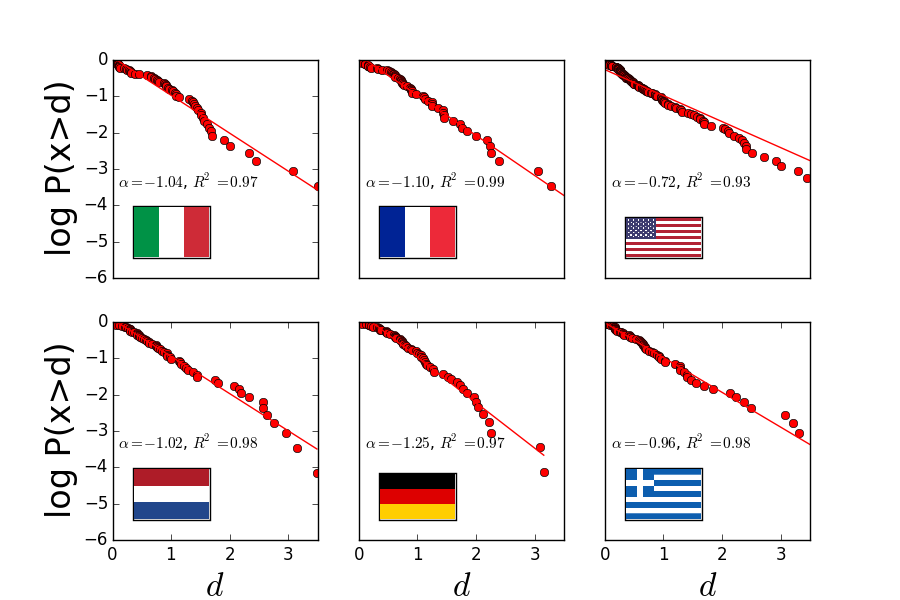
\includegraphics[width=0.95\textwidth]{figs_io/6panel_data.png}
  \caption{Outdegree distribution of several countries. The data shown
    is the counter cumulative in semilog scale, along with the linear
    fit. The largest outliers of our data, the US and Germany, are
    shown here.}
  \label{fig:6countries}
\end{figure}

\begin{figure}[!ht]
  \centering
  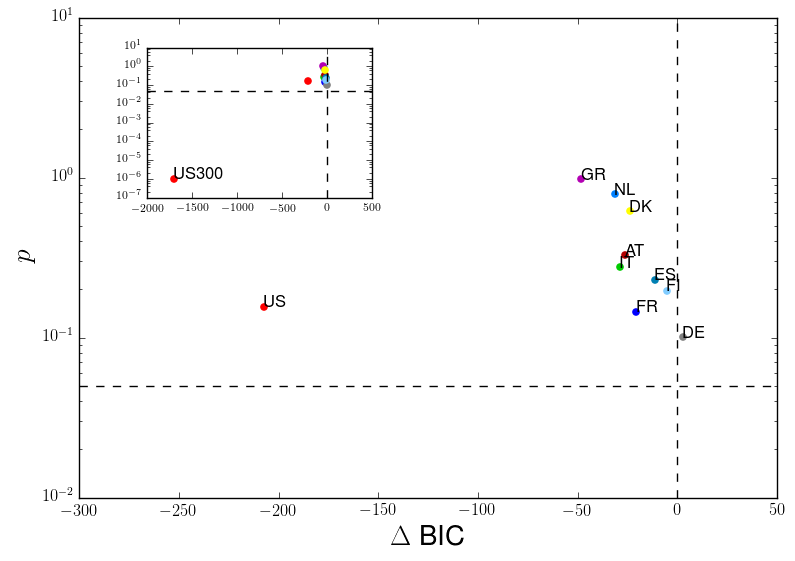
\includegraphics[width=0.95\textwidth]{figs_io/bic_pval_countries.png}
  \caption{Countries sorted by $\Delta$BIC of gaussian vs exponential
    (x axis) and probabilities of KS distance against exponential (y
    axis). Inset: same plot with the US $M=300$ level of
    disaggregation included. Dashed lines indicate $\Delta$BIC$=0$ and
    $p=0.05$.}
  \label{fig:BICpval}
\end{figure}

Figure \ref{fig:BICpval} depicts $p$ versus $\Delta$BIC for all the countries studied. We see that the bulk of the EU countries lie together in a
small cluster of the graph, indicating that the exponential hypothesis
is a very good fit for them. This is further confirmed
by putting the finer resolution data for the United States
(represented by the US300 point) in the same plane: the disaggregated
distribution is a very strong outlier compared to the coarser data.

A more careful analysis at the ``exponential bulk'' shows that the
main outliers are the US data, that exhibits a distribution bending
upwards in the semi-log plot of Figure \ref{fig:6countries}, and
Germany with a degree distribution bending downward. This motivated us
to carry out the BIC test between the exponential distribution
hypothesis and a stretched exponential defined as

\begin{equation}
\label{eq:stretched_exp}
P(d)=A(b,\theta)e^{-b x^\theta},\qquad b,\theta>0
\end{equation}

The result of this BIC test is shown in Figure
\ref{fig:theta_pval_data}, where the shaded region is where the
exponential ($\theta = 1$) is preferred to the stretched exponential
($\theta \neq 1$). We see that all countries analysed lie in this
region, with the exception of the US -- that is best fitted with $\theta<1$ -- and
Germany, Spain and Finland -- that are best fitted with $\theta>1$.

An exponential degree distribution across most of the countries under
study is of major relevance because the average degree of these
datasets is set to one by the normalisation requirement $d_\mu'=1$,
and the distribution of maximal entropy consistent with this
constraint is the exponential distribution. Since this is the least
informative distribution given the constraints we have, this suggests
that all the details of the input-output economics at the microscopic scale
have been washed out in the aggregation process.

Of course, the fact that this is the least informative doesn't mean
there is no information available. One can learn important things
about the economies in the aggregated dataset by looking at the relative 
importance of the different sectors. For example, among the
high degree products, ``Financial services'', ``Legal and accounting
services'' and ``Chemicals and chemical products'' are the highest
ranking ones, whereas, ``Imputed rents of
owner-occupied dwellings'' and ``Retail trade services'' have zero
degree in all countries. One can also look at the structural
differences between countries: in France, for example, products of
``Security and investigation services; office administration; office
support and other business support services'' are twice as used as in
Italy (degree of 3 vs 1.69), whereas in Italy,
``Electricity, gas, steam and air-conditioning'' are twice as depended
upon as in France (degree 4 vs 2). Yet the fact that the distribution of
degree takes a form consistent with maximum entropy, suggests that
the distribution carries no specific information on the economy. 
We shall now argue that this information is actually "lost in aggregation"
by looking at how the degree distribution evolves at different level of aggregation.


\section{Loss of information via aggregation}
\label{sec:aggreg} 

The above results show that aggregated data have a less informative
distribution of degrees. Indeed, for the most disaggregated data
available -- the 2007 US economy with $M=382$ -- we find that the
distribution of degrees is further away from the exponential
distribution with respect to the US data with $M=64$ sectors (see
point US300 in Fig. \ref{fig:theta_pval_data}).  At the other extreme,
if at a certain level of aggregation the distribution is exponential,
when we aggregate further, we expect the distribution to converge to a
Gaussian limit, because the degree at the coarser level is the sum of
the degrees at the finer one. This is appropriate if the degrees are
weakly dependent random variables, which in turn depends on how the
aggregation process is carried out, i.e. which sectors are put
together at the finer scale.  To answer the question of whether the
loss of information depends on the manner in which the aggregation is
carried out we will artificially aggregate the goods in the Use and Make tables
described in Section \ref{sec:IO} by collapsing pairs of goods into a
single one, ie, if we collapse $\mu_1$ and $\mu_2$ into $\mu$ the new
Use matrix would be $N$ by $M-1$ and would have $U_{i\mu} = U_{i\mu_1}
+ U_{i\mu_2}$. We would like to compare aggregation in two extreme
cases \emph{(i) random}: we choose $\mu_1, \mu_2$ randomly and
\emph{(ii) ranked}: we choose the two most correlated goods via
Spearman rank of the $M - U$ matrix, so that goods that highly
correlate in the usage as inputs - outputs by the industries will be
aggregated together first. In loose terms, as suggested by the
previous argument, we expect a faster loss of information
(i.e. convergence to the exponential distribution) when the
aggregation is carried out without taking into account the structure
of the data. As we'll discuss, this has practical consequences,
because a standardised aggregation method that has to be applied to
many countries, such as the one used in EU, may determine a faster
convergence to an uninformative distribution than a method that is
tailored to fewer countries (the one used by the US, Canada and
Mexico).

\begin{figure}[!ht]
  \centering
  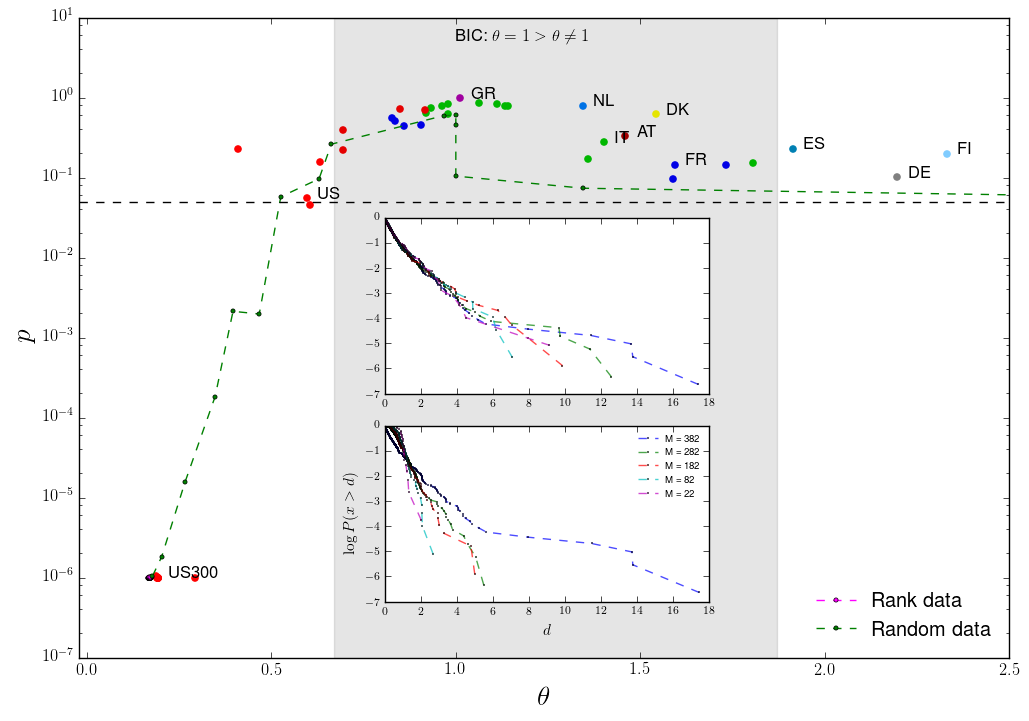
\includegraphics[width=0.95\textwidth]{figs_io/theta_pval_data_agg_w_inset.png}
  \caption{Countries in the $(p, \theta)$ plane, along with the two
    artificial aggregation processes carried out on the US300 data. The shaded
    area is the region where the BIC favors exponential distribution
    ($\theta = 1$) as opposed to stretched ($\theta \neq
    1$).
    \emph{Insets}: Evolution of the degree distribution under rank
    (top) and random (bottom) aggregation.}
  \label{fig:theta_pval_data}
\end{figure}


\subsection{Empirical data: the case of the US}

We take the most disaggregated data available, the 2007 US economy
with $M=382$ sectors, and aggregate according to the two methods
described above.  The results in the $(p, \theta)$ plane
are shown in figure \ref{fig:theta_pval_data}. We observe that we indeed obtain very different behavior depending on how the aggregation is carried out. Interestingly, the artificial method closer to the BEA classification system is random aggregation, while the ranked aggregation never converges to the exponential distribution. This is
because it creates a very dense ``supergood'' with positive entries in
all of its Make and Use tables that has a very high degree, while the
rest of the goods are left with sparse entries in the
tables. Nonetheless, ranked aggregation preserves the maximum degree
observed in the economy, as shown in the insets of figure
\ref{fig:theta_pval_data}.

\subsection{Random economies}

We now turn to the question of whether one can reproduce the maximum entropy degree distribution with a simple model and what is the effect of aggregation in those artificial economies. For that, we will build Input-Ouput matrices for economies in the Random Linear Economy model described in chapter \ref{cha:RLE}.

\begin{figure}[!ht]
  \centering
  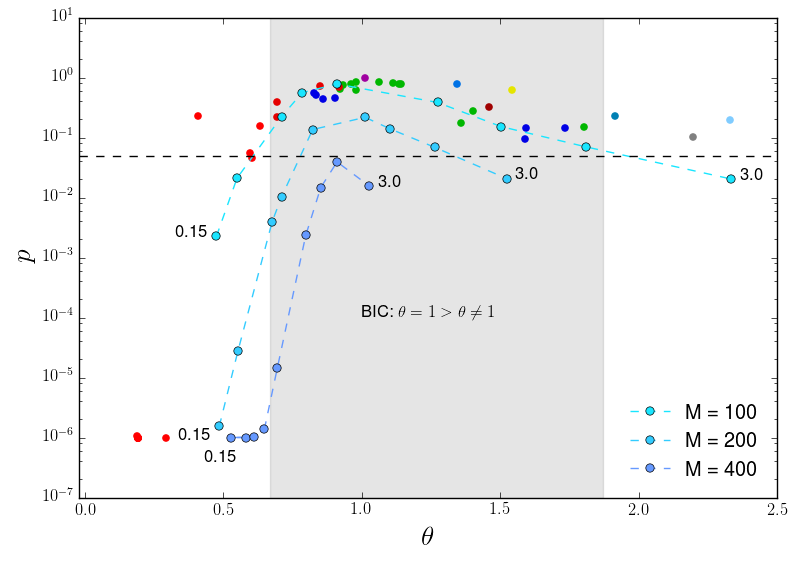
\includegraphics[width=0.95\textwidth]{figs_io/theta_pval_model_orig.png}
  \caption{Comparison of the Random Economies with real data in the
    $(p, \theta)$ plane. The model is shown for three quantity of goods
    $M$, each curve represents the model results with the number of firms per good $n = N/M$ varying from 0.15 to 3. We observe that the model parameters are able to represent the range of economies well, however these results are not scale dependent, not converging to a well defined limit when we increase $M$ keeping $n$ constant.}
  \label{fig:theta_pval_model_orig}
\end{figure}


The Use and Make tables can be defined for the Random Economies as
a function of the price vector $p$, the scales of production $s$ and the technologies $\xi$. The total amount of a good $\mu$ a firm $i$ produces is given by $p_\mu s_i \xi_i^\mu$ for all goods $\mu$ that have positive $\xi_i^\mu$. Likewise, the amount used is given by the negative terms in $\xi_i$. We define them the Use and Make tables as:

\begin{equation}
  \label{eq:io_4}
  U_{i\mu} = p_\mu s_i \left|\xi_i^{\mu, -}\right|, \quad M_{i\mu} =
  p_\mu s_i \xi_i^{\mu, +},
\end{equation}
where $\xi_i^{\mu,+} = \xi_i^\mu$ if $\xi_i^\mu > 0$ and $0$
otherwise. Likewise, $\xi_i^{\mu, -} = \xi_i^\mu$ only if
$\xi_i^\mu < 0$. One thing to note is that, unlike real Input-Output data, in
the model a good is never used as an input to itself. Therefore either $M_{i\mu}$ is positive or $U_{i\mu}$, never
both and $D_{\mu\mu} = 0$ for all goods, unlike the data where the
diagonal terms of the $D$ are usually large. Yet this holds only at the
microscopic level: for the model, $D_{\mu,\mu}$ can be nonzero after
aggregation.


We observe in numerical simulations that the properties of the model's direct requirement matrices are similar to the
real world data. For $M=100$, the degree distributions of the random
economies are remarkably similar to the ones given by real data, if we
vary $N$ (and therefore $n$), as shown in Figure
\ref{fig:theta_pval_model_orig}. When the repertoire of technologies is
relatively small (small $N$) compared to the number of goods, the
model exhibits a broad distribution of degrees reminiscent of the US
data whereas when $N$ increases the distribution becomes less heavy
tailed. However, as can be seen in Figure \ref{fig:theta_pval_model_orig}, these degree distributions are dependent on the
parameters $M$, $N$ and $\epsilon$ in a complicated manner and do
not converge to a well defined limit as $M$ diverges with $n=N/M$ and
$\epsilon$ finite.

Yet the behavior of the model under aggregation is quite similar to
that observed in real data, as seen in Figure
\ref{fig:theta_pval_model_agg} and degree distribution converges to
the same cluster of noninformative exponential distributions of the EU
/ US aggregated data.

\begin{figure}[!ht]
  \centering
  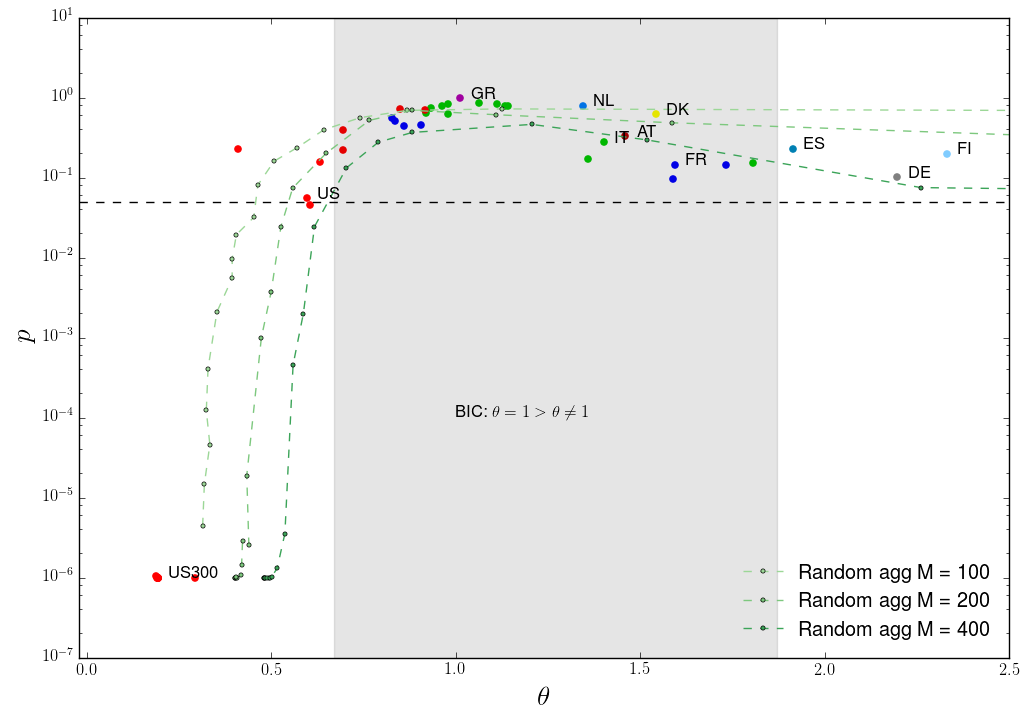
\includegraphics[width=0.95\textwidth]{figs_io/theta_pval_model_agg.png}
  \caption{Comparison of the randomly aggregated Random Economies with real data in the
    $(p, \theta)$ plane. The model always starts at one single
    realization of the Make and Use tables (as opposed to averaged
    over the disorder) for $n=0.15$ and randomly aggregated.}
  \label{fig:theta_pval_model_agg}
\end{figure}


\subsection{Consequences of aggregation}

The above results provide good evidence that the method by which the
BEA aggregates the sectors in the US economy is closer to a random
aggregation that to a ranked one. The Eurostat has no data publicly
available for a higher level of disaggregation, yet comparing the
degree distributions at the $M\sim 64$ sectors level suggests that EU
aggregation is also performed in an effectively random manner. In this
section we explore the consequences of this washing out of
information.

The direct requirement graph allows us to characterize the structural
susceptibility of the economy to shocks and perturbations: the
distribution of degrees give us a notion of how asymetric are the
dependencies between goods and what fraction of the production
capabilities depend on a single (or a few) goods. One of the ways
aggregation can lose information is if it doesn't take the good
degrees into account when selecting pairs to merge. Then, it will
likely happen that high degree goods will be aggregated with low
degree goods, possibly creating a good that has an degree in between the original ones\footnote{One must keep in mind that because aggregation is linear on the Use and Make tables, not in the Direct Requirement table, it's not true that the good resulting from the aggregation of a set of goods will have degree equal to the average of this set.}. This will gradually be responsible for eliminating the heavy tail of the distribution, masking the very high dependencies which are the most important for determining shock volatility. We test this hypothesis by calculating the normalized standard deviation of the ranks bundled together at each step: we define the rank of a good as its position in an ordered list of degrees, 1 being the lowest degree good and $M$ the highest degree good, then given a new good $\mu' = \sum_{k=1}^K \mu_k$ and given by  $r(\mu)$, then we the standard deviation of the aggregation as

\begin{equation}
    \frac{\sigma(\mu')}{M} = \frac{1}{M} \sqrt{\sum_{k=1}^M \left(r(\mu_k) - \bar{r}\right)^2}
\end{equation}

The results of $\frac{\sigma}{M}$ for each bundle of goods aggregated at each step using the three methods are shown in Figure \ref{fig:chi}. One sees that, as expected, this spread in the degrees being aggregated is highest when the random method is used and lowest when rank based is used, with the actual category based classification in between.

The degrees, however, are a first order measure for the spread of
perturbations which does not take cascade effects into account: the
perturbation of a good will impact the production of its dependencies
which may also have very high degree, amplifying the initial shock. In
\cite{Acemoglu12}, the authors show that the norm of a quantity similar to
the Bonacich centrality vector \cite{JacksonBook} is a lower bound for
the aggregated fluctuations generated by random, independent shocks
acting on the whole economy. This vector is given by

\begin{equation}
  \label{eq:centrality}
  \chi = \frac{\alpha}{M}(\mathds{I} - (1-\alpha) D)^{-1}\cdot \mathds{1},
\end{equation}
where $\mathds{I}$ is the identity matrix, $\mathds{1}$ is a vector
with all entries equal to one and $\alpha \in (0,1)$. The argument
used by Acemoglu \emph{et al} in \cite{Acemoglu12} is that in a
balanced structure in which random independent shocks in the whole
network average themselves out, as $M$ increases the norm
$\|\chi\| (M)$ of the vector should decrease proportionally to $\sqrt{M}$, but if
one calculates the $\chi$ both for the $M=382$ and $M=71$ aggregation
levels of the BEA data, the decrease is approximately
$~n^{\frac{1}{8}}$, considerably slower than a balanced economy. This
is interpreted as an evidence that the US economy is more susceptible
than expected to shocks.

\begin{figure}[!ht]
  \centering
  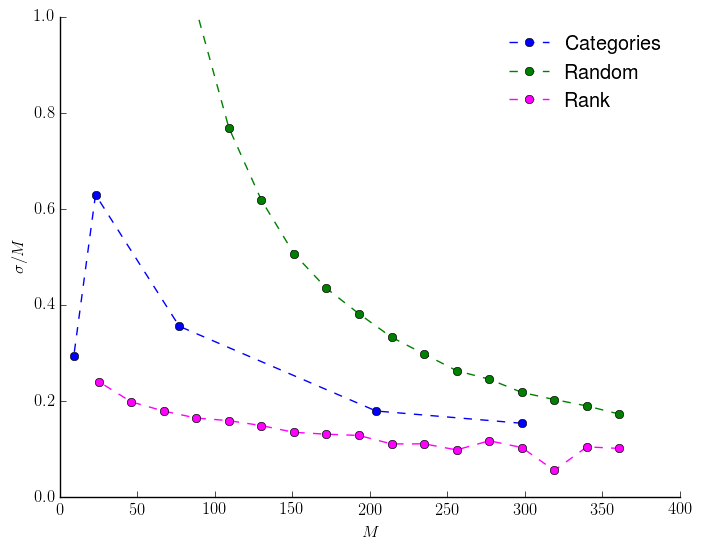
\includegraphics[width=.48\textwidth]{figs_io/cv_degree.png}
  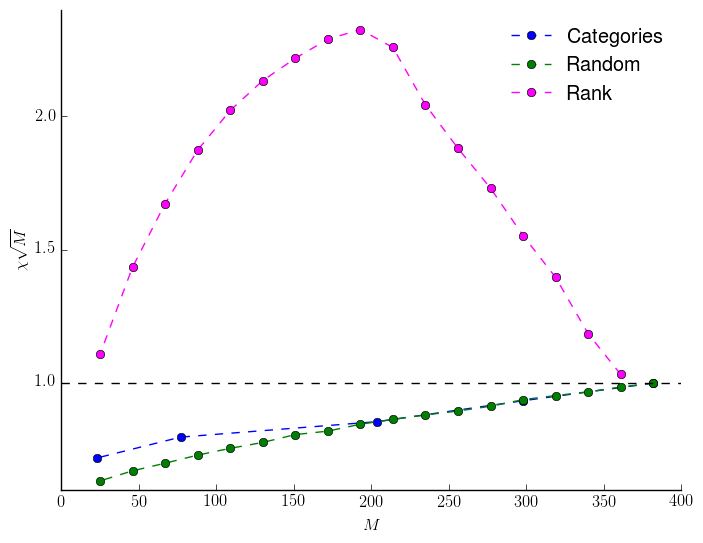
\includegraphics[width=.48\textwidth]{figs_io/susc_data.png}
  
  \caption{\textbf{(Left)} Scaled standard deviation $\sigma / M$ for
    the degree rank of the goods that are considered a single good at
    each aggregation step. The random aggregation has the highest
    average standard deviation, while the rank based has the
    lowest. This further corroborates the idea that random (and
    category) aggregation washes out high dependencies by merging them
    with low ones. \textbf{(Right)} Normalized average Bonacich
    centrality $\chi\sqrt{M}$ \cite{Acemoglu12}. This quantity should
    be constant if aggregated shocks have a limited effect (because
    $\chi$ decreases with $\sqrt{M}$) Here we see that networks with
    random aggregation have a different susceptibility to shocks than
    rank based ones, in particular, random (and category based)
    aggregation has $\chi$ decreasing slower than $\sqrt{M}$,
    exacerbating the effects of shocks.}
  \label{fig:chi}
\end{figure}


We calculate the same quantity for the three aggregation types
and plot the normalized (by $M=382$) $\|\chi\|\sqrt{M}$ on figure
\ref{fig:chi}. This quantity should be constant if $\|\chi\|$ decreases
proportionally to $\sqrt{M}$, as expected in a balanced structure, and
increasing with $M$ if it falls slower than that. We see on the graph
that random aggregation, again, generates a slightly unbalanced
structure, but the behaviour under rank aggregation is very different,
first increasing rapidly with $M$ (i.e., what would indicate a very
susceptible structure), but then it falls equally fast. We interpret
this result as a clear evidence that the direct requirement graph
properties are not simply a characteristic of the economy itself, but
very dependent on the method used for aggregation.

The important takeaway from this analysis is that sector
classification changes the whole structure of Direct Requirement
matrices. If the current classification methods serve a specific
purpose not related to the input-output structure, then when analysing
the Input-Output tables one must take into account that systemic risks like the
ones discussed in \cite{Acemoglu12} are aggregated away and
underrepresented.

However, if the purpose of building the Input-Output tables is to
make an assessment of which sectors are structural and which ones are
not, then the way the classification
hierarchy is built must change. The current one is, for a lack of better word,
``thematic''. Food is always aggregated together, so are the byproducts of
mining and so are services. These do not take into account the fact
that strawberries and eggs may have wildly different centralities and
degrees in the input-output network. The Spearman rank method we used
is a highly artificial way to aggregate, but it still preserves the
high degree of dependence of the US economy in certain crucial sectors.


\section{Conclusion}

The economic woes of the last decade brought to surface the importance
of identifying firms, and sectors, that are highly structural and from
which a sizeable portion of the production depends, and properly taking
steps to make the economy less vulnerable. However, we have shown here
that if one is not careful when organizing and classifying economic
data, this information can be lost.

Our results also show that at an intermediate scale of aggregation,
economies exhibit universal statistical properties that suggest that a
Statistical Mechanics approach may be feasible. In particular, the
study of the aggregation properties of models of large economies can
provide valuable hints on building a theory of macroeconomic
behaviour based on microeconomic interactions.

Going back to the question of what is the purpose of the current
classification scheme. From the BEA handbook we read

\begin{quote}
  The I-O tables are used to study changes in the structure of the
  U.S. economy and to assess the impact of specified events on
  economic activity.
\end{quote}

However, both the North American Industry Classification System
(NAICS), used by the BEA to construct the US data, and the NACE, used
by Eurostat, have as main purpose and advantage the usage of a uniform
classification for all the countries and their respective statistical
agencies in North America and the European Union. It is not surprising,
therefore, that the effects of their aggregation are closer to a
random process than to a method that takes the underlying data structure into
account.


\chapter{When does inequality freeze an economy?}
In this chapter we will describe the work on inequality on a zero intelligence based economy.



\section{Introduction}

The debate on wealth inequality has a long history, dating back at least to the work of Kutznets \cite{Kuznets1955} on the u-shaped relationship of inequality on development. Much research has focused on the relation between inequality and growth (see e.g. \cite{PerssonTabellini1994}). Inequality has also been suggested to be positively correlated with a number of indicators of social disfunction, from infant mortality and health to social mobility and crime \cite{TheSpirit}.

\begin{figure}%[htbp]
\centering
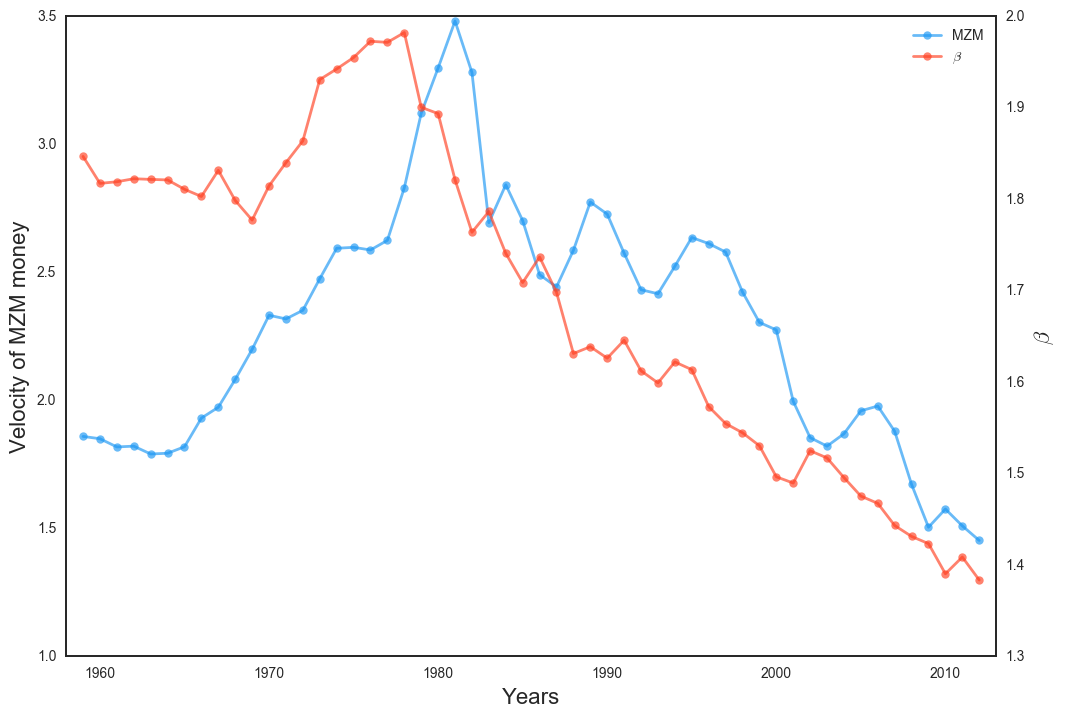
\includegraphics[width=0.59\textwidth]{figs_ineq/data_1.png}
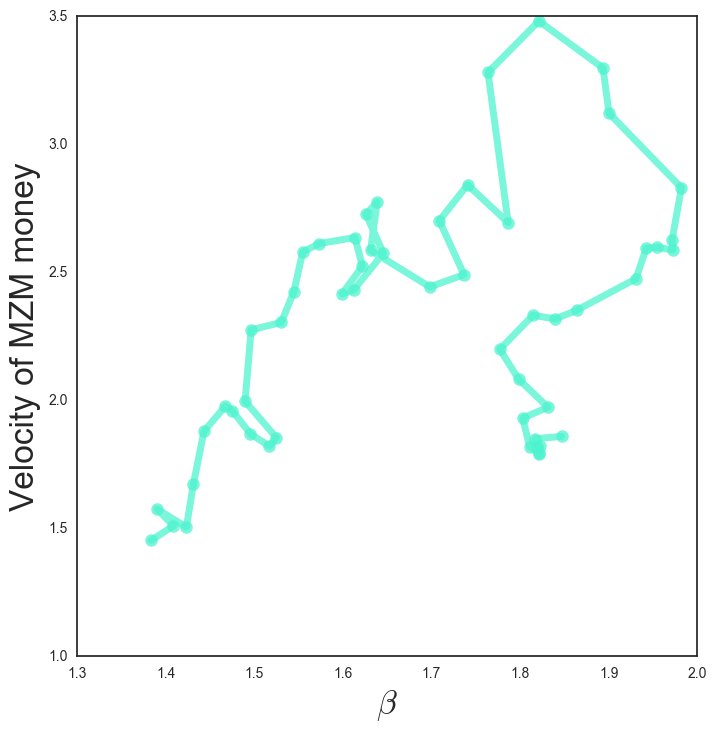
\includegraphics[width=0.39\textwidth]{figs_ineq/data_2.png}
\caption{\textbf{(Left)} Velocity of money of MZM stocks (left y-axis) and Pareto exponent $\beta$ of the wealth distribution (right y-axis) as a function of time. Both time series refer to the US, the data on the money velocity is retrieved from \cite{FRED}, the data on the wealth distribution is taken from \cite{SaezZucman2016}. \textbf{(Right)} MZM velocity of money as a function of $\beta$, for the same data.} 
\label{Fig:data}
\end{figure}

The subject has regained much interest recently, in view of the claim that levels of inequality have reached the same levels as in the beginning of the 20th century \cite{Piketty2001}. Saez and Zucman \cite{SaezZucman2016} corroborate these findings, studying the evolution of the distribution of wealth in the US economy over the last century, and they find an increasing concentration of wealth in the hands of the 0.01\% of the richest. Figure \ref{Fig:data} shows that the data in Saez and Zucman \cite{SaezZucman2016} is consistent with a power law distribution $P\{w_i>x\}\sim x^{-\beta}$, with a good agreement down to the 10\% of the richest (see caption\footnote{\label{foot:beta fit}
Ref. \cite{SaezZucman2016} reports the fraction $w_>$ of wealth in the hands of the $P_>=10\%, 5\%, 1\%, 0.5\%, 0.1\%$ and $0.01\%$ richest individuals.  If the fraction of individuals with wealth larger than $w$ is proportional to $P_>(w)\sim w^{-\beta}$, the wealth share $w_>$ in the hands of the richest $P_>$ percent of the population satisfies $w_>\sim P_>^{1-1/\beta}$ (for $\beta>1$). Hence $\beta$ is estimated from the slope of the relation between $\log P_>$ and $\log w_>$, shown in the inset of Fig. \ref{Fig:data} (left) for a few representative years. The error on $\beta$ is computed as three standard deviations in the least square fit. 
}). The exponent $\beta$ has been steadily decreasing in the last 30 years,  
reaching the same levels it attained at the beginning of the 20th century ($\beta=1.43\pm 0.01$ in 1917).


One of the most robust empirical stylised fact in economics, since the work of Pareto, is the observation of a broad distribution of wealth which approximately follows a power law.  What is interesting about it is that such a power law distribution of wealth does not require sophisticated assumptions on the rationality of players as we have dealt so far in this thesis, but it can be reproduced by a plethora of simple models (see e.g. \cite{bouchaud2000wealth,Yakovenko2009Review,Gabaix2009,Sornette2013}), in which it emerges as a typical behaviour, i.e. as the behaviour that the system exhibits with very high probability, within quite generic settings. This relates to the often made criticism that the neo-classical approach of Economics, aimed at explaining global behaviour in terms of perfectly rational actors, has largely failed \cite{SMD30,BouchaudCrisis,KirmanBook}. Yet, persistent statistical regularities in empirical data suggest that a less ambitious goal of explaining economic phenomena as emergent statistical properties of a large interacting system may be possible, without requiring much from agents' rationality \cite{Gode1993,Smith2003}. 

Taking inspiration from such independence from economic actor rationality, we aim in this work to study inequality via a zero intelligence agent model, in which agents with different capital trade goods randomly in a market. Rather than focusing on the determinants of inequality, we focus on a specific consequence of inequality: its impact on liquidity. There are a number of reasons why this is relevant. First of all, the efficiency of a market economy essentially resides on its ability to allow agents to exchange goods. A direct measure of the efficiency is the number of possible exchanges that can be realised or equivalently the probability that a random exchange can take place. This probability quantifies the ``fluidity'' of exchanges and we shall call it \textbf{liquidity} in what follows. This is the primary measure of efficiency that we shall focus on. 

Secondly, liquidity, as intended here, has been the primary concern of monetary polices such as Quantitative Easing aimed at contrasting deflation and the slowing down of the economy, in the aftermath of the 2008 financial crisis. A quantitative measure of liquidity is provided by the \textbf{velocity of money} \cite{IFisher}, measured as the ratio between the nominal Gross Domestic Product and the money stock\footnote{The data reported in this chapter concerns the MZM (money with zero maturity), the broadest definition of money stock that includes all money market funds. We refer to \cite{FRED} for further details.} and it quantifies how often a unit of currency changes hand within the economy. As Figure \ref{Fig:data} shows, the velocity of money has been steadily declining in the last decades, with a clear correlation to the level of inequality. The current work in this chapter suggests that this decline and the increasing level of inequality are not a coincidence. Rather the former is a consequence of the latter. 

Without clear yardsticks marking levels of inequality that seriously hamper the functioning of an economy, the debate on inequality runs the risk of remaining at a qualitative or ideological level. The main finding of the work presented in this chapter is that, in the simplified setting of the model presented, there is a sharp threshold beyond which inequality cripples the economy. More precisely, when the power law exponent of the wealth distribution approaches one, liquidity vanishes and the economy halts because all available (liquid) financial resources concentrate in the hands of few agents. This provides a precise, quantitative measure of when inequality becomes too much. 

Our main goal is thus to isolate the relation between inequality and liquidity in the simplest possible model that allows us to draw sharp and robust conclusions. Specifically, the model is based on a simplified trading dynamics in which agents with a Pareto distributed wealth randomly trade goods of different prices.  Agents receive offers to buy goods and each such transaction is executed if it is compatible with the budget constraint of the buying agent. This reflects a situation where, at those prices, agents are indifferent between all feasible allocations. The model is in the spirit of random exchange models (see e.g. \cite{Foley1994, SjurFlam2012, Yakovenko2009Review}), but our emphasis is not on whether the equilibrium can be reached or not. In fact we show that the dynamics converges to a steady state, which corresponds to a maximally entropic state where all feasible allocations occur with the same probability. Rather we focus on the allocation of cash in the resulting stationary state and on the liquidity of the economy, defined as the fraction of attempted exchanges that are successful. Since the wealth distribution is fixed, the causal link between inequality and liquidity is clear in the simplified setting we consider.

Within our model, the freezing of the economy occurs because when inequality in the wealth distribution increases, financial resources (i.e. cash) concentrate more and more in the hands of few agents (the wealthiest), leaving the vast majority without the financial means to trade. This ultimately suppresses the probability of successful exchanges, i.e. liquidity. 


\section{The model}
\label{sec:modelDescription}

We introduce an inequality trading model consisting of an economy with $N$ agents, each with wealth $c_i$, $ i = 1, \ldots, N$. There are $M$ objects to be traded among the agents in the economy and each object $m = 1, \ldots,M$ has a price $\pi_m$. A given allocation of goods among the agents is described by an $N\times M$ allocation matrix $\mathcal{A}$ with entries $a_{i,m} = 1$ if agent $i$ owns good $m$ and zero otherwise, but agents can only own baskets of goods that they can afford, i.e. whose total value does not exceed their wealth. The wealth of an agent not invested in goods corresponds to the cash (liquid capital) $\ell_i$ that agent $i$ has available for trading, ie,

\begin{equation}
c_i -  \sum_{m=1}^M a_{i , m} \pi_m =\ell_i\ge 0, \quad\quad i=1,\ldots,N,
\label{eq:1}
\end{equation}

Therefore the set of feasible allocations -- those for which $\ell_i\ge 0$ for all $i$ -- is only a small fraction of the $M^N$ possible realizations of the allocation matrices $\mathcal{A}$. 

The dynamics are similar to those typical of zero-intelligent agent-based models in economics and are described as following: starting from a feasible allocation matrix $\mathcal{A}$, at each time step a good $m$ is picked uniformly at random among all goods. Its owner then attempts to sell it to another agent $i$ also drawn uniformly at random among the other $N-1$ agents. If agent $i$ has enough cash to buy the product $m$, that is if $\ell_i \ge \pi_m$, the transaction is successful and his cash decreases by $\pi_m$ while the cash of the seller increases by $\pi_m$, otherwise the transaction fails, with no possibility of an object being divided. The total capital $c_i$ of agents does not change over time, so $c_i$ and the good prices $\pi_m$ are quenched parameters of the model. We reemphasize that there are no decisions to be made by the agents, they have no utility function to maximize and simply accept trades when selected if they have enough cash.

A crucial property of these dynamical rules is that the stochastic transition matrix $W(\mathcal{A}\to\mathcal{A}')$ is symmetric between any two feasible configurations $\mathcal{A}$ and $\mathcal{A}'$: $W(\mathcal{A}\to \mathcal{A}') = W(\mathcal{A}'\to \mathcal{A})$ and any feasible allocation $\mathcal{A}$ can be reached from any other feasible allocation $\mathcal{A}'$ by a sequence of trades. This implies that the dynamic satisfies the detailed balance condition:

\begin{align}
W(\mathcal{A} \to \mathcal{A}') P(\mathcal{A}) = W(\mathcal{A}'\to \mathcal{A})P(\mathcal{A}'),  \quad \forall \mathcal{A}, \mathcal{A}'
\end{align}
with a stationary distribution over the space of feasible configurations that is uniform, ie, $P(\mathcal{A})= \frac{1}{A}$, where $A$ is the number of feasible allocations. This is a consequence of the symmetric transition rates, and would be the same for every trading rule that has $W(\mathcal{A}\to \mathcal{A}') = W(\mathcal{A}'\to \mathcal{A})$. In fact, the current trading rules employed in this model are a particular case of a general rule for which we first select a subset of $n$ agents, $2 \leq n \leq N$, then we pick a random good from these $n$ agents and try to trade it with the remaining $n-1$ agents, automatically accepting if the chosen buyer has enough cash to purchase it. This rule may sound cryptic, but it's common in the particular cases of $n=N$, which is the current one described in the model, and for $n=2$, in which we first pick two consumers and then try to exchange a random good among themselves. All of these rules generate the same stationary distribution.

% TODO: cite below for wealth dist, or check if its in the intro

For the distribution of agents capital, we focus on realisations where the wealth $c_i$ is drawn from a Pareto distribution $P\{c_i> c\} \sim c^{-\beta}$, for $c>c_{\min}$ for each agent $i$, which is compatible with many empirical observations of real world wealth distribution. The parameter $\beta$ will be the main quantity to be explored in this work because it regulates the different levels of inequality among the agents. To compare different economies, the ratio between the total wealth $C=\sum_i c_i$ and the total value of all objects $\Pi=\sum_{m}\pi_m$ will be kept fixed. Because $C$ is a random variable with potentially very high variance, the number of goods $M$ is realization dependent, we will populate the economy with as many items as needed to keep the ratio $C/\Pi$ constant, which will be described in details late. In order to have feasible allocations, it hold that $C>\Pi$.

For the goods, we are going to limit the analysis to cases where the $M$ objects are divided into a small number of $K$ classes with $M_k$ objects per class ($k=1,\ldots,K$), where objects belonging to class $k$ have the same price $\pi_{(k)}$. If $z_{i,k}$ is the number of object of class $k$ that agent $i$ owns, then the budget condition given by equation \eqref{eq:1} takes the form

\begin{equation}
c_i =  \sum_{k=1}^K z_{i , k} \pi_{(k)} + \ell_i
\end{equation}

As with standard statistical mechanics systems, we will throughout this work assume that the economy is very large, that is, $N, M \to \infty$ but with the ratio $C/\Pi$ constant. This will allow us to calculate the probability distribution of goods $P (z_i^k | c_i)$ for each agent in an exact manner in the large system (thermodynamic) limit. In the next section we will solve the master equation and find the distribution of goods as a function of capital $c_i$. As it will be shown, the main result of this model is that the flow of goods among agents becomes more and more congested as inequality increases until it halts completely when the Pareto exponent $\beta$ tends to one.


\section{The case of one type of good}

We begin our analysis by the simplest case in which there is only one type of good being traded, i.e., $K=1$ with prices $\pi_k = \pi$, but the results shown will extend for the general setting. A formal approach to this problem would consist in writing the complete Master Equation that describes the evolution for the probability $P(z_1,\ldots, z_N)$ of finding the economy in a state where each agent $i=1,\ldots,N$ has a specific number $z_i$ of goods. We would then take the sum over all values of $z_j$ for $j\neq i$ to derive the Master Equation for a single agent with wealth $c_i$. However, due to the almost mean-field like nature of the interactions, we can directly write the detailed balance conditions for a single marginal $P_i(z)$, which will be solvable with a few approximations that exploit the large system size. The detailed balance equation for a single agent is

\begin{equation}
    \Delta P_i(z) =  P_i(z+1 \to z) P_i(z+1) + P_i(z-1 \to z) P_i(z-1) - \left (P_i(z \to z + 1) P_i(z) + P_i(z \to z - 1) P_i(z) = 0 \right)
    \label{eq:full_master_equation_k1}
\end{equation}

However, there are further steps we can take to simplify this equation: we are looking for the stationary distribution of $P_i(z)$ knowing that all the feasible allocations $\mathcal{A}$ are equiprobable and the probability rates are symmetric, $W(\mathcal{A}\to \mathcal{A}') = W(\mathcal{A}'\to \mathcal{A})$. We therefore can solve the detailed balance equation using a stronger condition in which, not only it has to hold that the probability of coming to a state $z$ has to be equal to the probability of leaving it, as equation \eqref{eq:full_master_equation_k1} states, but instead requiring that the probability of going from a specific state $z$ to another $z'$ is equal to the probability of going from $z'$ to $z$. If we take $z' = z + 1$, we have

\begin{equation}
P_i(z + 1) P_i(z + 1 \to z) = P_i(z) P(z \to z + 1)
\end{equation}

The transition probabilities are given as follows: $P_i(z + 1 \to z)$ is the probability of selling a good, which is composed of two independent events: \emph{(i)} a good of agent $i$ is chosen as the good to be traded, which happens with probability $\frac{z+1}{M}$ and \emph{(ii)} the transaction is successful, ie, the chosen recipient is able to afford the good. This happens with probability $p^s$, whose form we will write later. Therefore $P_i(z + 1 \to z)$ is given by $\frac{z+1}{M}  p^s$. $P_i(z \to z+1)$, on the other hand, is the probability that the agent buys a good, which happens if a good he doesn't own if chosen, which has probability $\frac{M - z}{M}$, he is picked as buyer, with probability $\frac{1}{N-1}$ and has enough cash to purchase it. This means the probability is truncated by a term $1-\delta_{z, m_{i}}$, where $m_{i}=\floor{c_i / \pi}$ is the maximum number of goods which agent $i$ can buy with his wealth $c_i$. If $z=m{i}$ then he cannot afford the item and the probability is zero.

We put it all together and make two large size approximations: $\frac{1}{N-1} \approx \frac{1}{N}$ and $\frac{M -z}{M} \approx 1$, that is, we used the fact that $N \gg 1$ and $z \ll M$. The first assumption holds by definition, but the latter breaks down if $\beta < 1$, as we will discuss later. We finally have the simplified detailed balance equation for agent $i$


\begin{equation}
P_i(z+1)  \frac{z+1}{M}  p^s =  P_i(z) \frac{1}{N} \left(1-\delta_{z, m_{i}}\right) ,\qquad z=0,1,\ldots, m_i
\label{eq:master_equation_simple_k1}
\end{equation}

The probability of success $p^s$ for the trade is given by

\begin{align}
p^s & =  1-\frac{1}{N-1}\sum_{j\neq i} P(z_j=m_j|z_i=z)\\
 & \cong  1-\frac{1}{N}\sum_{j} P_j(m_j)\qquad (N,M\gg 1)\label{eq:ps_1Guy}
\end{align}
where the last relation holds because when $N,M\gg 1$ the dependence on $z$ and on agent $i$ becomes negligible. This is important because it implies that for large $N$ the variables $z_i$ can be considered as independent, i.e., $P(z_1,\ldots, z_N)=\prod_i P_i(z_i)$, and the problem can be reduced to that of computing properties from the marginals $P_i(z)$. The probability $p^s$ will be the main dynamical quantity of interest in this model, as an indicator of market activity: when $p^s$ is close to 1, all trades succeed and we consider the market liquid, with goods trading hand frequently. When $p^s \to 0$, most transactions fail and the market becomes frozen.

We can plug an Anzats in equation \eqref{eq:master_equation_simple_k1} and see that it is solved by a truncated Poisson distribution with parameter $\lambda = M / (N p^s)$:

\begin{equation}
P_i(z) = \frac{1}{Z_i} \left( \frac{\lambda^{z}}{z!}\right) \Theta\left(m_i - z \right),
\label{Eq:ME_solution_1Good}
\end{equation}
where $Z_i$ is a normalization factor that can be determined by $\sum_{z} P_i(z) = 1$. The value of $p^s$, or equivalently of $\lambda$, can be found only in certain approximations of equation \eqref{eq:ps_1Guy}, which we will show later.


%%%% TWO CLASSES OF AGENTS
From the stationarity distribution \eqref{Eq:ME_solution_1Good}, we see that the most likely value of $z$ for an agent with $m_i=m$ is given by

\begin{equation}
z^\ast(m)  = \argmax_z  P(z)=
\begin{cases}
    m, & \text{ if } m \leq \lambda \\
    \lambda, & \text{ if } m \geq \lambda
  \end{cases}.
  \label{Eq:cases_ztyp}
\end{equation}

This provides a natural distinction between cash-poor agents -- those with $m \leq \lambda$ --  that often cannot afford to buy any other object, and cash-rich ones -- those with $m> \lambda$ --  who typically have enough cash to buy further objects. We can run computer simulations for the model and compare the goods distribution after equilibrium against the theoretical predicted, the results are shown in figure \ref{Fig:Picturesque_RichPoor_transition_beta}. We indeed observe these two types of agents in the simulations, which agree very well with the prediction. The inset shows the cash distribution $P_i(\ell/\pi)$ (where $\ell/\pi = c_i/\pi - z$ represents the number of goods they are able to buy) for some representative agents. While cash-poor agents have a cash distribution peaked at $0$, the wealthiest agents have cash in abundance. When $\lambda\gg 1$, the distribution $P_i(z)$ is sharply peaked around $z^{\text{mode}}(m)$ so that its average is $\langle z\rangle\simeq z^{\text{mode}}(m)$. Then the separation between the two classes becomes rather sharp, as is the case for Figure \ref{Fig:Picturesque_RichPoor_transition_beta}.

\begin{figure}%[htbp!]
\centering
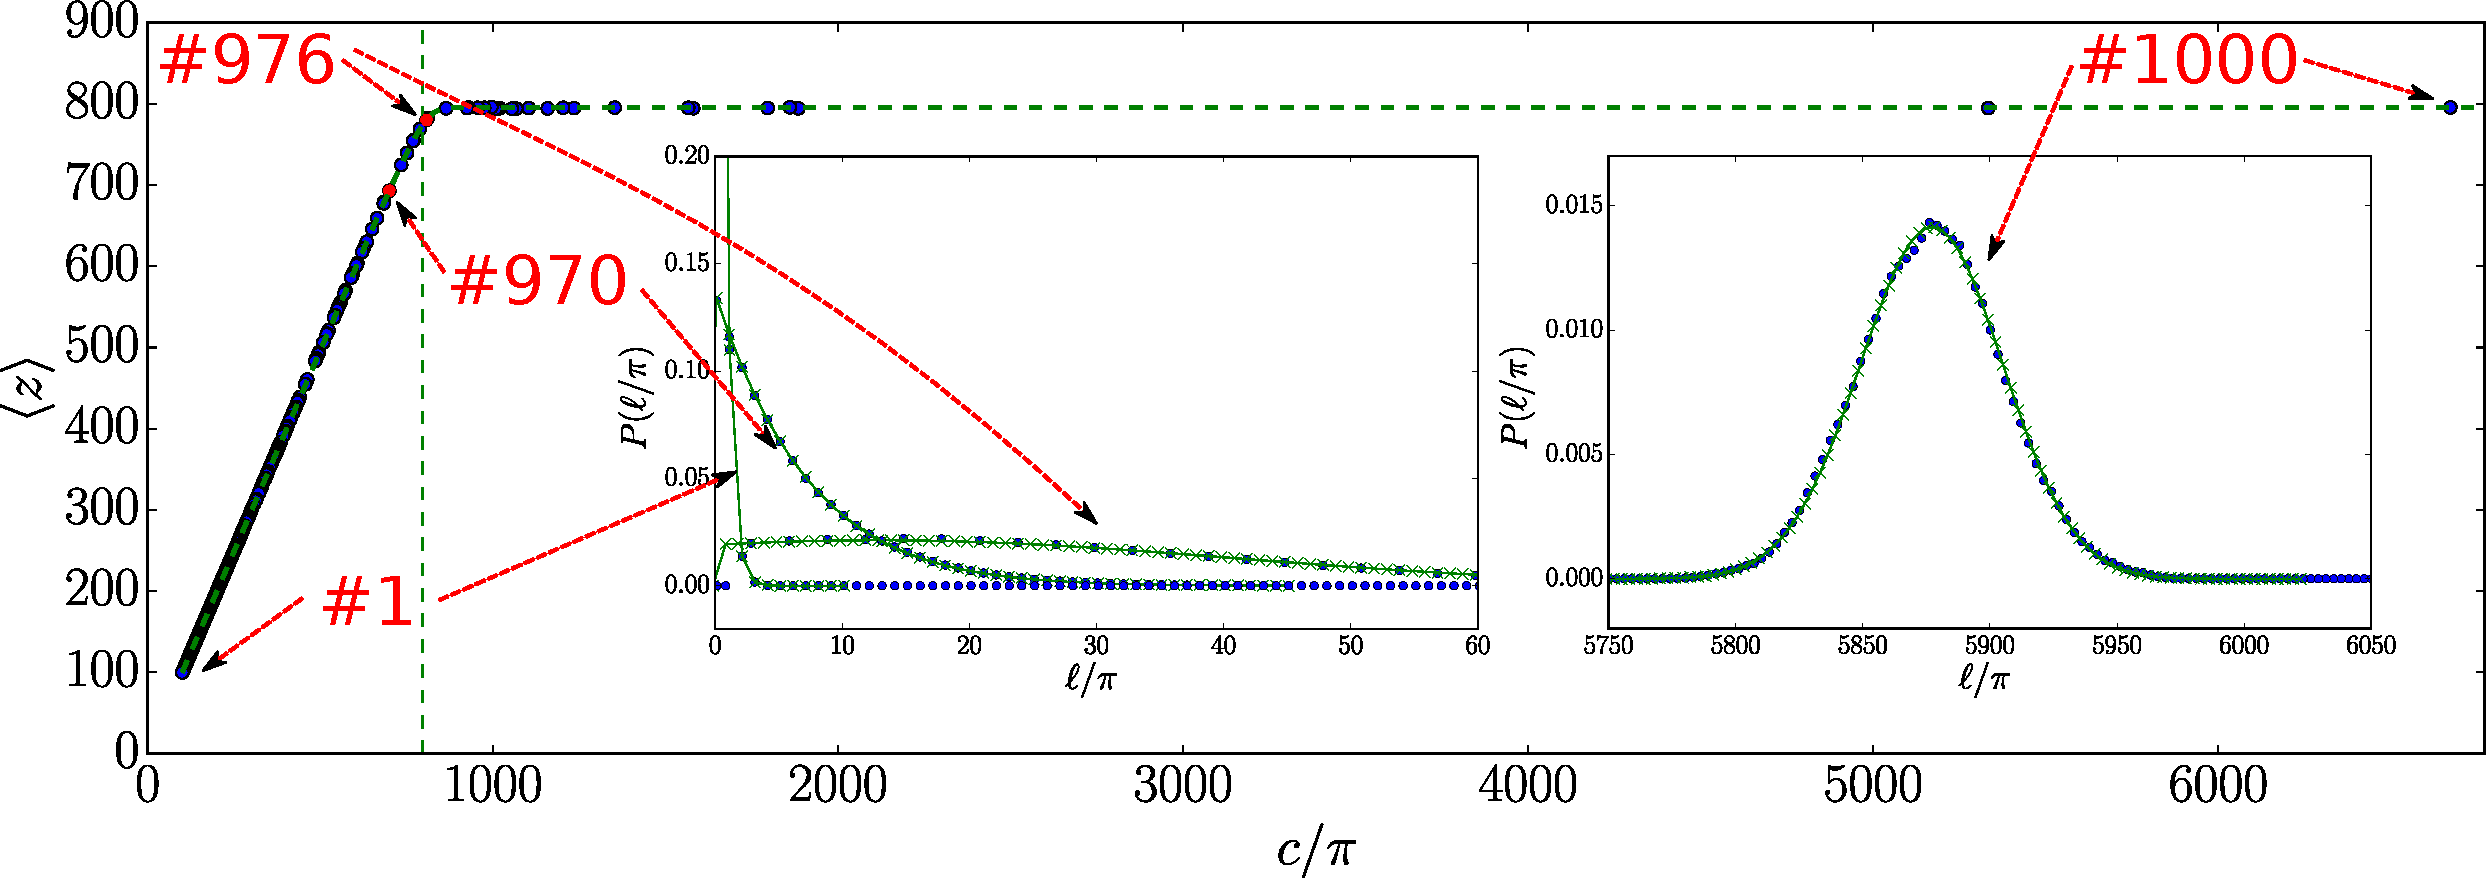
\includegraphics[width=\textwidth]{figs_ineq/fig3_ownership_average_beta=1p80_e=1p10-byHand.pdf}
\caption{\textbf{(Main)} Average number of owned goods in an economy with a single type of good, $N=10^3$ agents, $\beta=1.8$, $M\approx 2 . 10^5$ and $C/\Pi=1.1$. Points $\{(\langle z \rangle_i,c_i)\}_{i=1}^{N}$ denote the average composition of capital for different agents obtained in Monte Carlo simulations, compared with the analytical solution obtained from the Master Equation (green dashed line) given by equation \eqref{Eq:ME_solution_1Good}.
The vertical dashed line at $c^{(1)}\simeq 7.98=M/N p^s_1$ indicates the analytically predicted value of the crossover wealth that separates the two classes of agents. \textbf{(Insets)} Cash distributions $P_i(\ell)$ of the indicated agents. 
}
\label{Fig:Picturesque_RichPoor_transition_beta}
\end{figure}

In terms of wealth, we can use the threshold shown in equation \eqref{Eq:cases_ztyp} to define the threshold wealth $c^{(1)}$ for which the poor are defined as those with $c_i<c^{(1)}$ whereas the rich ones have $c_i>c^{(1)}$. This threshold wealth is given by the initial capital an agent requires to have $m = \lambda$. Because all goods have the same price, this is simply given by $\lambda \pi$. So the threshold wealth for the two classes $c^{(1)}$ is given by

\begin{equation}
c^{(1)} = \lambda \pi = M \pi/(N p^s)
\label{eq:c1}
\end{equation}

We can compute $p^s$ by using equation \eqref{eq:ps_1Guy}, $p^s = 1 - \frac{1}{N} \sum_{i=1}^{N} P_i(z = m_i)$, and approximating the probability to be on a threshold $P_i(z=m_i)$ by

\begin{align}
P_i(z=m_i) = 
\begin{cases}
\left( 1 - \frac{m_i}{\lambda} \right) & \text{ for } m_i \ll \lambda \\
0 & \text{ for } m_i > \lambda
\end{cases}
\label{eq:k1_saturated_prob}
\end{align}

The first case can be understood by noting that in the limit $m_i \ll \lambda$ we have the approximation

\begin{equation}
P_i(z=m_i) = \frac{\lambda^{m_i} \frac{1}{m_i!}}{\sum_{x=0}^{m_i} \lambda^x \frac{1}{x!}} = \frac{1}{1 + \frac{m_i}{\lambda} + \frac{m_i (m_i -1)}{\lambda^2} + \ldots} \simeq  \left( 1 - \frac{m_i}{\lambda} \right),
\end{equation}

Assuming this approximation to be valid for all $m_i < \lambda$ is clearly a bad assumption for all agents with $m_i$ close to $\lambda$. However the wealth is power law distributed and so the weight of agents with $m_i \sim \lambda$ is negligible in the sum over all agents in equation \eqref{eq:app_ps_analytic0}. The accuracy of this approximation increases when the exponent of the power law $\beta$ decreases and the mass of agents with capitals around $\lambda$ vanquishes. 

We use equation \eqref{eq:k1_saturated_prob} and write $m_i \approx \frac{c_i}{\pi}$ to rewrite equation \eqref{eq:ps_1Guy}:

\begin{equation}
\label{eq:ps_first_approx}
p^s = 1 - \frac{1}{N} \sum_{i=1}^{N} P_i(z = m_i) \simeq 1 - \frac{1}{N} \sum_{i=1}^N \left(1 - \frac{c_i}{\lambda \pi}\right) \Theta\left(c_i - \lambda \pi \right)
\end{equation}

Because we have a very large number of agents, we are able to transform the sum over the agents into an integral over the capital $c$, with density equal to the capital distribution, ie, we replace

\begin{equation}
\frac{1}{N} \sum_i c_i \to \int_1^\infty c \beta c^{-\beta - 1} dc
\end{equation}

Thus when we truncate by $c_i \leq \lambda \pi = c^{(1)}$ we get

\begin{equation}
\label{eq:app_ps_analytic1}
p^s = 1 - \int_1^{c^{(1)} = \lambda \pi} dc\, \beta c^{-\beta - 1} \left( 1 - \frac{c}{\lambda \pi} \right) .
\end{equation}

This is an implicit expression for $p^s$, since it appears on the left hand side of the equation and also inside the integral, because $\lambda = \frac{M}{N p^s}$, which makes it intractable to solve analytically. 

However, we can get good insights on the behavior of $p^s$ by again exploiting the fact that we are assuming a very large system and take $N, M \to \infty$. In this limit, $\lambda$ can be replaced by its expected value on the realizations, i.e., for finite system sizes, $M/N$ is a random variable that depends on the realization of the capital distribution due to the fixed constant $\Pi/C$, but in the limit we can replace $M$ by it's expected value, $\Pi/\pi$ and $N$ by $C / \langle c \rangle$, where $\langle c \rangle$ is the expected capital per agent, which is given by the average of the beta distribution, $\langle c \rangle = \beta/(\beta-1)$. For finite $N$, this is only a reasonable approximation if $\beta \gg 1$, and breaks down in the limit $\beta \to 1^+$ due to the infinite variance of the capital distribution, but it should be accurate for all $\beta > 1$ in the limit $N \to \infty$. Using the approximation on \eqref{eq:c1} and replacing $\lambda = c^{(1)} / \pi$, we have:

\begin{equation}
\frac{M}{N \lambda} \to \left \langle \frac{M}{N} \right \rangle \frac{\pi}{c^{(1)}} = \frac{\Pi}{C} \frac{\beta}{\beta - 1} \frac{1}{c^{(1)}}
\end{equation}

So the equation for $p^s$ is, by the definition of $\lambda$:

\begin{equation}
 \label{Eq:ps_correct}
p^s = \frac{M}{N \lambda} = \frac{\Pi}{C} \frac{\langle c \rangle}{c^{(1)}},
\end{equation} 
which gives us $p^s$ but as a function of $c^{(1)}$, which we still don't know. But now that this is independent of $p^s$, we can put this expression back into \eqref{eq:app_ps_analytic1} and carry out the integration to get an analytic form for $c^{(1)}$:

\begin{equation}
\frac{\Pi}{C} \frac{\langle c \rangle}{c^{(1)}} = {c^{(1)}}^{-\beta} \left( \frac{1}{1-\beta} \right) - \frac{\beta}{1 - \beta } \frac{1}{c^{(1)}},
\end{equation}

Solving for $c^{(1)}$ we have

\begin{equation}
\label{Eq:c1_correct}
c^{(1)} = \left[\beta \left(  1 - \frac{\Pi}{C}\right) \right]^{1/(1 - \beta)}.
\end{equation}

And replacing this back on equation \eqref{Eq:ps_correct} gives $p_s$ as a function of the intensive variables for the economy

\begin{equation}
p^s = \frac{\Pi}{C}\frac{\beta}{\beta - 1} \frac{1}{\left[\beta \left(1 - \frac{\Pi}{C}\right) \right]^{1/(1 - \beta)}}.
\end{equation}

\begin{figure}[!ht]
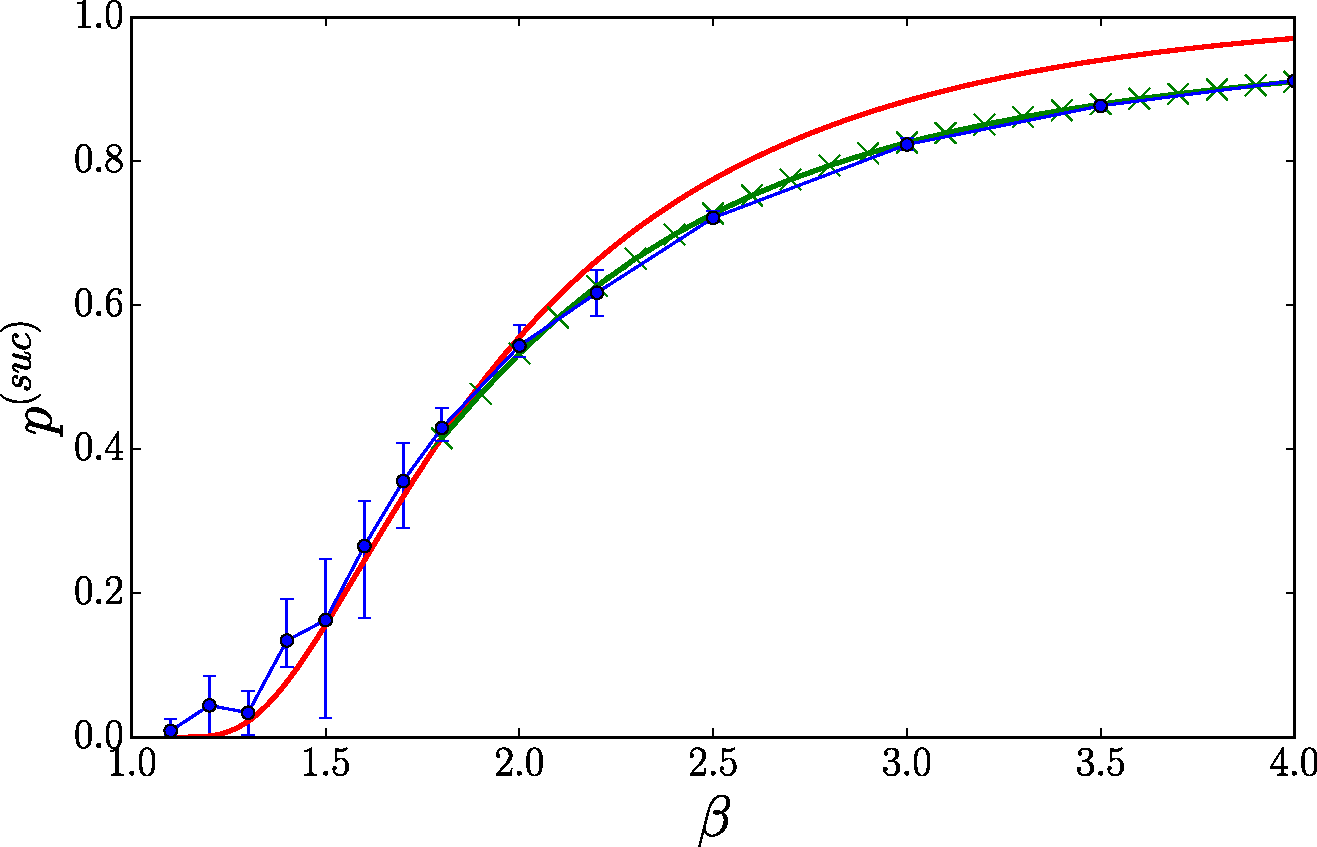
\includegraphics[width=\textwidth]{figs_ineq/fig_K=1_e=1p2_g=undef_ps_prediction_unadj.pdf}
\caption{Comparison between numerical simulations and analytical estimates for the success probability of transaction $p^s$ for one class of goods, as a function of the Pareto exponent $\beta$. The blue solid circles are the result  of Monte Carlo simulations performed for $N=10^5$ agents and averaged over 5 realizations, with the error bars indicating the min and max value of $p^s$ over all realizations. The red lines are the analytic estimates  according to equation \eqref{Eq:ps_correct}. The green crossed lines correspond to numerically solving the analytical solution  \eqref{Eq:ME_solution_2Goods} for a population composed of $N=64$ "agents".}
\label{Fig:ps_one_good}
\end{figure}

When the inequality in wealth becomes too large, in the limit $\beta \to 1^+$, $\langle c \rangle$ diverges, but within this approximation the threshold wealth $c^{(1)}$ diverges much faster. More precisely, we note that $\Pi/C<1$, so that $\beta ( 1- \Pi/C) \sim (1-\Pi/C)$ is a number smaller than 1 (yet positive). From equation \eqref{Eq:c1_correct}, we have $c^{(1)}\sim (1-\Pi/C)^{-1/(\beta-1)} \to \infty$ and therefore the liquidity $p^s$ vanishes as $\beta \to 1^+$. We now arrive at the main result of this work: when the distribution of capital gets too unequal, the probability of successful transactions vanishes and the economy freezes.

For finite $N$, this approximation breaks down when $\beta$ gets too close to or smaller than one, because $\langle c \rangle$ is ill-defined and in equation \eqref{Eq:ps_correct} it should be replaced with $1/N \sum_i c_i $, which strongly fluctuates between realizations and depends on $N$. An estimate of $p^s$ for finite $N$ and $\beta<1$ can be obtained by observing that the wealth $c^{(1)}$ that marks the separation between the two classes cannot be larger than the wealth $c_{\max}$ of the wealthiest agent. By extreme value theory, the latter is given by $c_{\max}\sim N^{1/\beta}$, with $a>0$. Therefore the solution is characterised by $ c^{(1)}=\pi \lambda\sim c_{\max}\sim N^{1/\beta}$. Furthermore, for $\beta<1$ the average wealth is dominated by the wealthiest few, i.e. $\langle c \rangle \sim N^{1/\beta-1}$ and therefore  $p^s \sim N^{1/\beta-1}/c^{(1)} \sim N^{-1}$. In other words, in this limit the cash-rich class is composed of a finite number of agents, who hold almost all the cash of the economy. In regimes such as this, not only the wealthiest few individuals own a finite fraction of the whole economy's wealth, as observed in \cite{bouchaud2000wealth}, but they also drain all the financial resources in the economy.
% TODO: explain iterative method


\section{The case of $K$ types of goods}

The analysis presented in the last section carries over to the general case in which $K$ classes of goods are considered, starting from the full Master Equation for the joint probability of the ownership vectors $\vec z_i=(z_{i,1}\ldots, z_{i,K})$ for all agents $i=1,\ldots,N$. For the same reasons as before, the problem can be reduced to that of computing the marginal distribution $P_i(\vec z_i)$ of a single agent. The main complication is that the maximum number $m_{i,k}$ of goods of class $k$ that agent $i$ can get now depends on how many of the other goods agent $i$ owns, i.e. $m_{i,k}(z^{(k)}_i)=\floor{(c_i-\sum_{k'(\neq k)} z_{i,k'} \pi_{(k')})/\pi_{{k}}}$, where $z^{(k)}_i=\{z_{i,{k'}}\}_{k'(\neq k)}$. 

Again, as with the single good case, because all transition rates are symmetric we can write the detailed balance condition in a stricter manner: the probability of leaving going to one specific state to another has to be the same as doing the reverse trajectory. In this case, however, all the exchanges are confined to a dimension in the $K$-dimensional space of ownership, ie, an agent can go from $z$ to either $z + \hat e_k$ or $z - \hat e_k$, where $\hat e_k$ is the vector with all zero components and with a $k^{\rm th}$ component equal to one, but not to $z + \hat e_k - \hat e_{k'}$. Therefore, the stationary distribution $P_i (z)$ has to satisfy the strict detailed balance condition for all $k$.

We write the probability of agent $i$ going from $z$ to $z + \hat e_k$ as $P_i (z \to z + \hat e_k) = \frac{M_k - z_k}{M} \frac{1}{N} \left(1-\delta_{z_k,m_{i,k}(z_{(k)})}\right)$, the exact analogous of the single good case. Likewise, $P(z + \hat e_k \to z) = \frac{z_k}{M} p^s_k$, where $p_s^k$ is the probability that a sale of an object of type $k$ is successful.

Putting it all together with the the approximations for the $N, M \to \infty$ limit, $\frac{1}{N-1} \approx \frac{1}{N}$ and $\frac{M_k - z_k}{M} \approx \frac{M_k}{M}$, assuming $z_k \ll M_k$, we have the detailed balance condition for goods of type $k$:

\begin{equation}
\label{Eq:MasterEq3_2Goods_1Guy}
P_i(\vec z+\hat e_k)\frac{z_k+1}{M}p^s_{k}=
P_i(\vec z)  \frac{M_k}{M} \frac{1}{N} \left(1-\delta_{z_k,m_{i,k}(z_{(k)})}\right) 
\end{equation}

It can easily be checked that a solution to this set of equations is given by a product of Poisson distributions with parameters $\lambda_k=M_k/(N p^s_{k})$, with the constraint given by equation \eqref{eq:1}

\begin{equation}
P_i(z_1,..., z_{K}) = \frac{1}{Z_i} \left( \prod_{k=1}^{K}\frac{\lambda^{z_k}_k}{z_k!}\right) \Theta\left(c_i - \sum_k^{K} z_k \pi_{(k)}\right)\,,
\label{Eq:ME_solution_2Goods}
\end{equation}
where $Z_i$ is a normalization factor obeying $\sum_{z_1}...  \sum_{z_{K}}  P_i(z_1, ..., z_{K}) = 1$. Each probability of success $p_k^s$ is given by

\begin{equation}
p^s_{k} = 1 - \frac{1}{N}\sum_{i=1}^N P\left(z_{i,k}=m_{i,k}(z_i^{(k)})\right)
\label{eq:ps_Kobjs}
\end{equation}

\begin{figure}
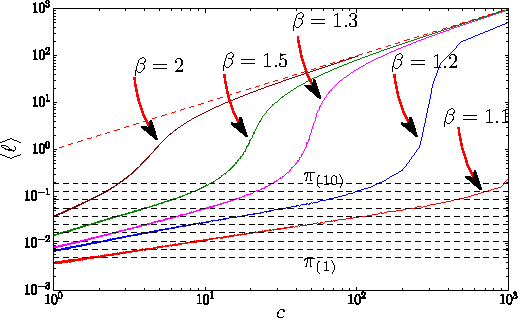
\includegraphics[width=\textwidth]{figs_ineq/cropping-liquidity_global-crop.pdf}
\caption{Time averaged cash $\langle \ell_i \rangle$ as a function of wealth $c_i$, from $\beta= 1.1$ to $\beta =2$  for a system of $N=10^5$ agents exchanging $K=10$ classes of goods ($\pi_{(k)}=\pi_{(1)}g^{k-1}$ with $g=1.5$, $\pi_{(1)}=0.005$, $M_k\pi_{(k)}=\Pi/K$ and $C/\Pi=1.2$). The dashed lines indicate the different prices of goods. Agents with $\langle \ell_i \rangle$ below the price of a good typically have not enough cash to buy it. Cash is proportional to wealth for large levels of wealth (see the upper straight red dashed line).}
\label{Fig:K10_classes}
\end{figure}


When the total number of objects per agent is large for any class $k$, we expect that $\lambda_1, ..., \lambda_K \gg 1$, and then the average values of $z_{i,k}$ are close to their most likely values, as in the single good case. This means that, as with the single good case, and agent with wealth $c_i < \lambda_k \pi_k = c^{(k)}$ will be saturated with goods of type $k'\leq k$ and won't be able to afford goods of type $k'' \geq k$. 

The consequence is that the population of agents now splits into $K$ classes, defined by the intervals $c_i \in [c^{(k-1)},c^{(k)}]$, each filled with objects cheaper than $k$ and unable to purchase more expensive ones. This structure into classes can be seen in the computer simulations of Figure \ref{Fig:K10_classes}, where we present the average cash $\langle \ell_i \rangle$ of agents as a function of their initial wealth $c_i$. The horizontal lines denote the prices $\pi_{(k)}$ of the different objects, and the intersections with the horizontal lines define the thresholds $c^{(k)}$.


\begin{figure}
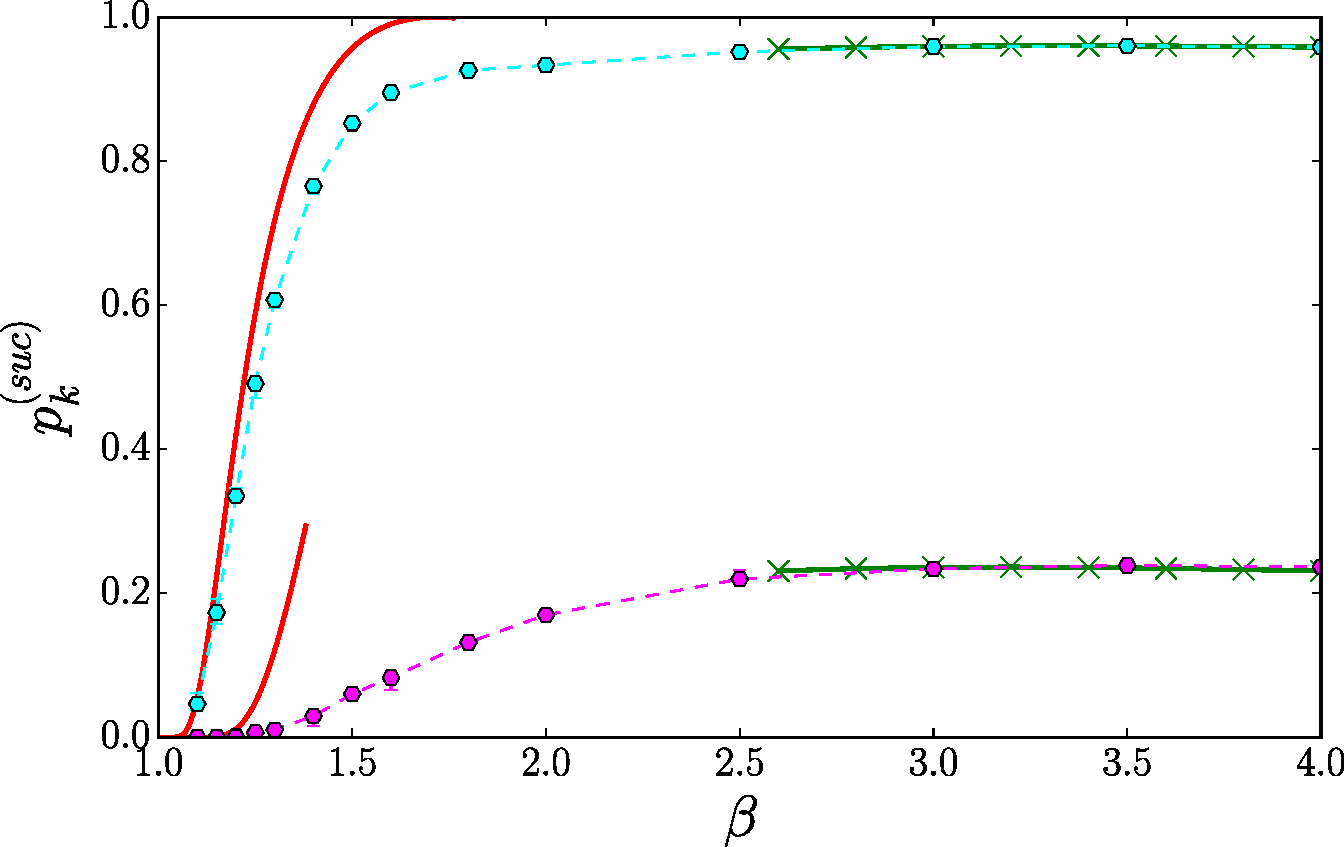
\includegraphics[width=0.8\textwidth]{figs_ineq/fig_K=2_e=1p2_ps_prediction_adjustedcapital.pdf}
\caption{Comparison between numerical simulations and analytical estimates of the success probability of transaction $p^s_k$ for two classes of goods as a function of the Pareto exponent $\beta$. The blue solid circles are the result  of Monte Carlo simulations performed for $N=10^5$ agents and averaged over 5 realizations, with the error bars indicating the min and max value of $p^s_k$ over all realizations. The red lines are the analytic estimates  according to equation \eqref{Eq:ps_and_ck_generalCaseAnyMathcalM1}. The green crossed lines correspond to numerically solving the analytical solution  \eqref{Eq:ME_solution_2Goods} for a population composed of $N=64$ agents.}
\label{Fig:summary_section_one_object}
\end{figure}

To see the effect of inequality in the trade activity, we must again find an analytical expression for the liquidities $p^s$, which are given by the following expression

\begin{equation}
p^s_{k} = 1 - \frac{1}{N}\sum_{i=1}^N P\left(z_{i,k}=m_{i,k}(z_i^{(k)})\right) = 1 - \frac{1}{N}\sum_{i=1}^N P_i(\text{not accepting good type k})
\label{eq:psk_sum}
\end{equation}

An analytic derivation for the $p_k^s$ and $c^{(k)}$ can be obtained only in the limit in which prices are well separated (i.e. $\pi_{(k+1)} \gg \pi_{(k)}$) and the total values of good of any class is approximately constant (we use $M_k\pi_{(k)}  = \Pi / K = {\rm const}$), because in this limit we expect to find a sharp separation of the population of agents into classes. When the prices are separated by an order of magnitude, then $M_1\gg M_2\gg \ldots \gg M_K$, which implies that the market is flooded with objects of the class $1$, which constantly change hands and essentially follow the laws found in the single type of object case. On top of this dense gas of objects of class $1$, we can consider objects of class $2$ as a perturbation (they are picked $M_2/M_1$ times less often). On the time scale of the dynamics of objects of type $2$, the distribution of cash is such that all agents with a wealth less than $c^{(1)}=\pi_{(1)}\lambda_1$ have their budget saturated by objects of type $1$ and typically do not have enough cash to buy objects of type $2$ nor more expensive ones. 
Likewise, there is a class of agents with $c^{(1)}<c_i\le c^{(2)}$ that will manage to afford goods of types $1$ and $2$, but will hardly ever hold goods more expensive that $\pi_{(2)}$, and so on. In this scenario we can write the probability of not accepting a good of type $k$ for an agent in the same linear fashion as in equation \eqref{eq:k1_saturated_prob} for $K=1$:

\begin{align}
P_i(\text{not accepting good type k}) = 
\begin{cases}
1 & \text{ for } m_i \leq \lambda_{k-1} \\
\left( 1 - \frac{m_i}{\lambda_k} \right) & \text{ for } \lambda_{k-1} < m_i < \lambda_k \\
0 & \text{ for } m_i \geq \lambda_k
\end{cases},
\end{align}

Then $p^s_k$ becomes a simple integral by employing the same steps taken on equations \eqref{eq:ps_first_approx}-\eqref{eq:app_ps_analytic1}.

\begin{equation}
p^s_{k} \simeq 1 - \int_{1}^{c^{(k-1)}} dc\, \beta c^{-\beta - 1} - \int_{c^{(k-1)}}^{c^{(k)}} dc\, \beta c^{-\beta - 1} \left( 1 - \frac{c}{c^{(k)}} \right) 
\end{equation}

In the $K$ goods case we now again replace $\frac{M}{N}$ by its average $\frac{\Pi}{C}\frac{\beta}{\beta - 1}\frac{1}{\pi}$ to find, from the definition of $\lambda_k$:

\begin{equation}
p_k^s = \frac{M_k}{N \lambda_k} = \frac{\Pi}{K C} \frac{\langle c \rangle}{c^{(k)}}
\end{equation}

Plugging this back again on the integral above, we get the general recurrence relation for $k$ goods.

\begin{equation}
c^{(k)} = \left(\beta \left( c^{(k-1)} \right)^{1-\beta} - \beta \frac{\Pi}{K C} \right)^{\frac{1}{1-\beta}}.
\end{equation}

Iterating, we write it as a function of the intensive variables 

\begin{equation}
c^{(k)} = \left[ \beta^k  - \left( \frac{\beta - \beta^{k+1}}{1-\beta} \right) \frac{\Pi}{K C} \right] ^{\frac{1}{1-\beta}},
\eqref{Eq:ps_and_ck_generalCaseAnyMathcalM1}
\end{equation}
 
And finally $p^s_k$ as a function of the intensive variables:

\begin{equation}
p_k^s = \frac{M_k}{N \lambda_k} \simeq \frac{\Pi}{K C} \frac{\langle c \rangle}{c^{(k)}}.
 \label{Eq:ps_and_ck_generalCaseAnyMathcalM2}
\end{equation}


\begin{figure}
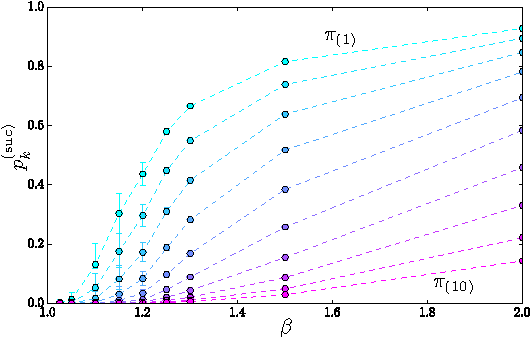
\includegraphics[width=\textwidth]{figs_ineq/cropping-K=10_e=1p2_g=1p5_ps_prediction_adjustedcapital-crop.pdf}
\caption{Liquidity of goods $\{p^s_k\}_{k=1}^K$  as a function of the inequality exponent $\beta$ for a system of $N=10^5$ agents exchanging $K=10$ classes of goods, with parameters $\pi_{(k)}=\pi_{(1)}g^{k-1}$ with $g=1.5$, $\pi_{(1)}=0.005$, $M_k\pi_{(k)}=\Pi/K$ and $C/\Pi=1.2$. Note that all success rates $p^s_k$ vanish when $\beta \to 1^+$.  The curves are ordered from the cheapest good (top) to the most expensive (bottom). The markers are the result of numerical simulations, with error bars indicating the minimum and maximum values obtained by averaging over 5 realizations of the wealth allocations.}
\label{Fig:K10_ps_beta}
\end{figure}

In the limit  $\beta \to 1^+$ of large inequality, close inspection\footnote{Note that the term in square brackets is smaller than one, when $\beta \to 1^+$.} of equation \eqref{Eq:ps_and_ck_generalCaseAnyMathcalM1} shows that $ c^{(k)}  \to \infty, \forall k$, 
which implies that all agents become cash-starved except for the wealthiest few. Since $p^s_{k}\sim \langle c \rangle /c^{(k)}$, this implies that all markets freeze: $p^s_{k}\to 0 , \forall k$.  The arrest of the flow of goods appears to be  extremely robust against all choices of the parameter $\pi_{(k)}$, as $p^s_{1}$ is an upper bound for the other success rates of transactions $p^s_{k}$. These conclusions are fully consistent with the results of extensive numerical simulations, as illustrated in figure \ref{Fig:K10_ps_beta}, in which we simulate an economy with $K=10$ classes of goods (see figure caption for details) and different values of $\beta$. As expected, for a fixed value of the Pareto exponent $\beta$ the success rate increases as the goods become cheaper, as they are easier to trade.  It also shows that trades of all classes of goods halt as $\beta$ tends to unity, which is when wealth inequality becomes too large, independently of their price.

\begin{figure}%[htbp]
\centering
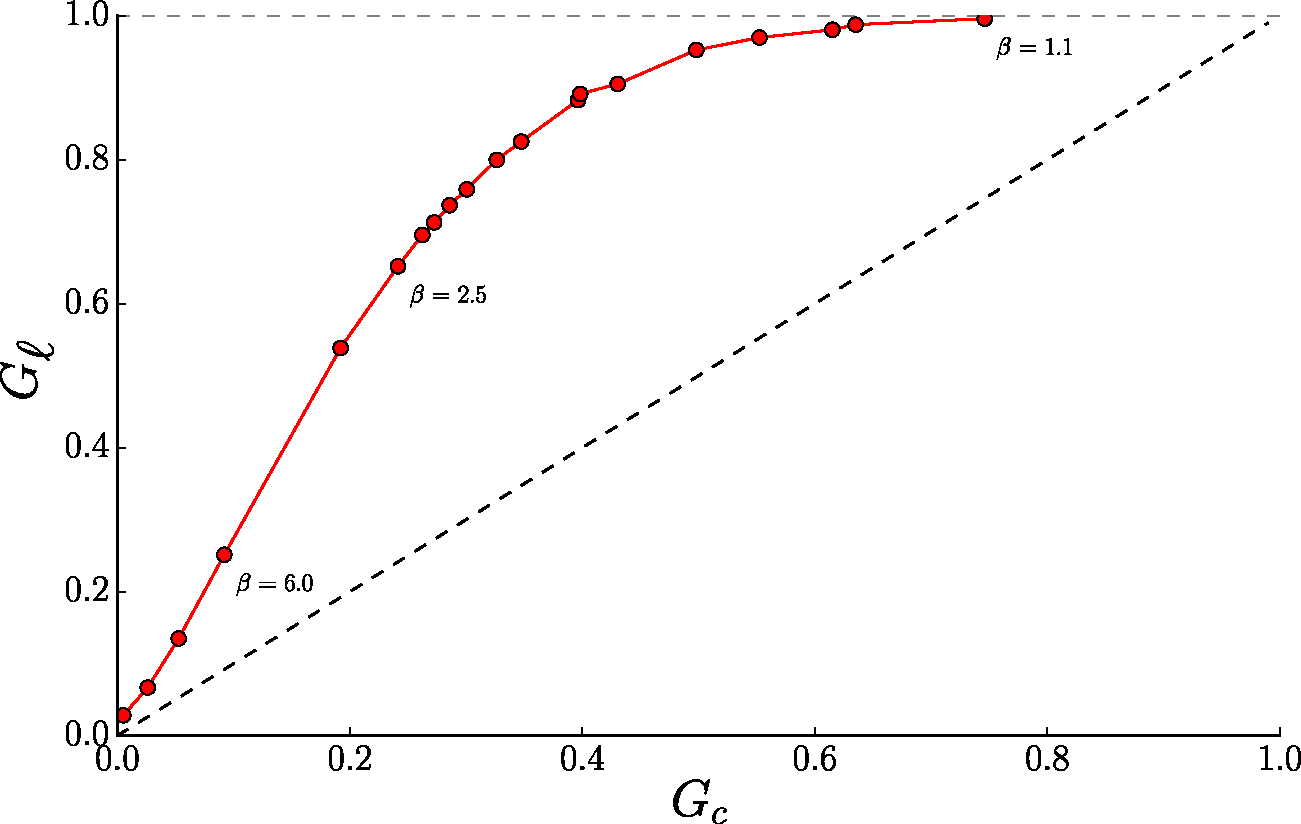
\includegraphics[width=\textwidth]{figs_ineq/gini_intro.pdf}
\caption{Gini coefficient $G_\ell$ of the cash distribution (liquid capital) in the stationary state as a function of the Gini $G_c$ of the wealth distribution, calculated through the numeral simulations of figure \ref{fig:K10_ps_beta}. The dashed line indicates proportionality between cash and wealth, in which case the inequality in both is the same.}
\label{fig:gini}
\end{figure}

An alternative way to interpret the freezing of the economy is to compare the cash and capital inequalities via their Gini coefficients. The Gini coefficient is a measure of inequality in a distribution: it is a function of the relative mean of the absolute difference among all the elements of the distribution, that is

\begin{equation}
G(\{x_i\}) = \frac{\sum_{i=1}^N \sum_{j=1}^N \| x_i - x_j \|}{2 N \sum_{i=1}^N x_i}
\end{equation}

The normalization term is so that the Gini coefficient has a support on $[0, 1]$ independent of the distribution, and it is invariant to scalings of the type $x_i \to \lambda x_i$. The measure is most commonly used in economics, for measuring income inequality among different countries, and a Gini coefficient of $0$ means perfect equality, where every point in a distribution is the same, whereas a Gini coefficient close to 1 means perfect inequality: only one point of the (presumed large) distribution is nonzero. 

For our economy, we plot on figure \ref{fig:gini} for various values of $\beta$ the Gini coefficient for cash $G_\ell$ as a function of the Gini coefficient for the capital $G_c$ in the $K=10$ system of figure \ref{Fig:K10_ps_beta}. The dashed line is the case where a certain inequality of capital implies the exact same inequality of cash. We see that the liquidity over concentrates, being much more unequal than the original capital distribution, approaching perfect inequality, i.e., concentrating in the hands of few agents much faster than the capital.


\begin{figure}%[htbp]
\centering
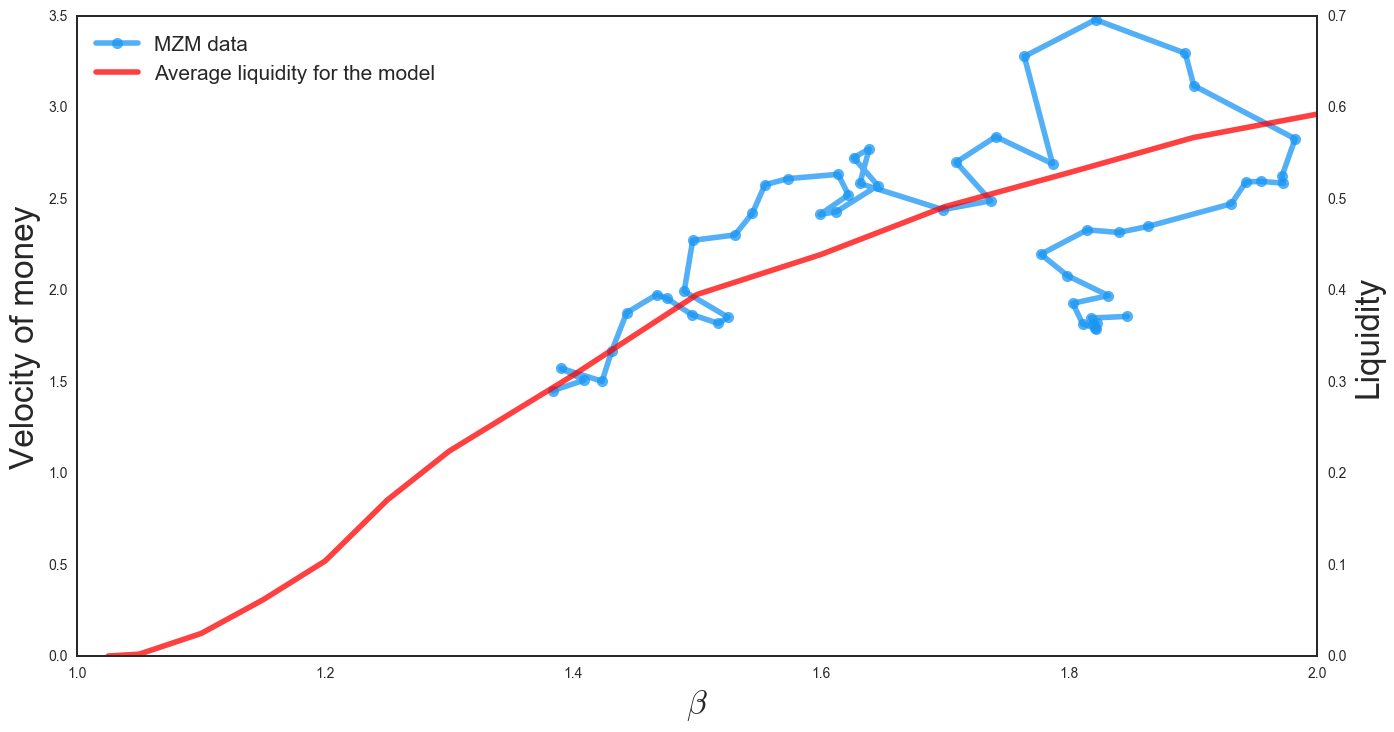
\includegraphics[width=\textwidth]{figs_ineq/data_model.png}
\caption{Comparison of MZM money velocity from the US data to average liquidity (as defined in equation \eqref{def:pavg}) calculated in the simulations of figure \ref{Fig:K10_ps_beta}.}
\label{fig:data_model}
\end{figure}

Note finally that $p^s_k$ quantifies liquidity in terms of goods. In order to have an equivalent measure in terms of cash that can be compared to the velocity of money described in the Introduction, we average $\pi_{(k)} p^s_k$ over all goods

\begin{equation}
\label{def:pavg}
\bar p^s=\frac{1}{\Pi}\sum_{k=1}^K M_k \pi_{(k)} p^s_k.
\end{equation}

This quantifies the frequency with which a unit of cash changes hand in our model economy as a result of a successful transaction. It's behaviour as a function of $\beta$ for the same parameters of the economy in Figure \ref{Fig:K10_ps_beta} is shown on Figure \ref{fig:data_model}. Even though we cannot make a one to one comparison with real world data, we see that the freezing we observe in the model due to high inequality is, at least qualitatively, corroborated by the data.


\section{Conclusions}
\label{sec:con}

We have introduced in this chapter a zero-intelligence trading dynamics in which agents have a Pareto distributed wealth and randomly trade goods with different prices. We have shown that this dynamics leads to a uniform distribution in the space of the allocations that are compatible with the budget constraints and when the inequality in the distribution of wealth increases, the economy converges to an equilibrium where typically (i.e. with probability very close to one) the less wealthy agents have less and less cash available, as their budget becomes saturated by objects of the cheapest type. At the same time this class of cash-starved agents takes up a larger and larger fraction of the economy, thereby leading to a complete halt of the economy when the distribution of wealth becomes so broad that its expected average diverges (i.e. when $\beta \to 1^{+}$). In these cases, a finite number of the wealthiest agents own almost all the cash of the economy. 

The model presented is intentionally simple, so as to highlight a simple, robust and quantifiable link between inequality and liquidity. In particular, the model neglects important aspects such as {\em i)} agents' incentives and preferential trading, {\em ii)} endogenous price dynamics and {\em iii)} credit. It is worth discussing each of these issues in order to address whether the inclusion of some of these factors would revert our finding that inequality and liquidity are negatively related. 

First, our model assumes that all exchanges that are compatible with budget constraints will take place, but in more realistic setting only exchanges that increase each party's utility should take place, just as we have approached in the rest of this thesis. Yet if the economy freezes in the case where agents would accept all exchanges that are compatible with their budget, it should also freeze when only a subset of these exchanges are feasible. The model also assumes that all agents trade with the same frequency whereas one might expect that rich agents trade more frequently than poorer ones. Could liquidity be restored if trading patterns exhibit some level of homophily, with rich people trading more often and preferentially with rich people? 

First we note that both these effects are already present in our simple setting. Agents with higher wealth are selected more frequently as sellers as they own a larger share of the objects. In spite of the fact that buyers are chosen at random, successful trades occur more frequently when the buyer is wealthy. So, in the trades actually observed the wealthier do trade more frequently than the less wealthy, and preferentially with other wealthy agents. Furthermore, if agents are allowed to trade only with agents having a similar wealth (e.g. with the $q$ agents immediately wealthier or less wealthy) it is easy to show that detailed balance still holds with the same uniform distribution on allocations. As long as all the states are accessible, the stationary probability distribution remains the same\footnote{
The dynamics changes and thus $p_k^{(\text{suc})}$ changes, in particular for goods more expensive than $\pi_{(1)}$, the seller is typically cash-rich and thus its neighbours are too. This can induce to have a liquidity of expensive goods higher than that of cheaper ones. However in the limit $\beta \to 1^{+}$, it is still true that cash concentrates in the hands of a vanishing fraction of agents, and there is still a freeze of the economy.}. Therefore, the model conclusions are robust with respect to a wide range of changes in its basic setting that would account for more realistic trading patterns. 

Secondly, it is reasonable to expect that prices will adjust -- i.e. deflate -- as a result of a diminished demand caused by the lack of liquidity. Within the model, the inclusion of price adjustment, occurring on a slower time-scale than trading activity, would reduce the ratio $\Pi/C$ (between total value of goods and total wealth), but it would also change the wealth distribution. Since the freezing phase transition occurs irrespective of the ratio $\Pi/C$, the first effect, though it might alleviate the problem, would not change the main conclusion. The second would make it more compelling, because cash would not depreciate as prices do, so deflation would leave 
wealthy agents -- who hold most of the cash -- even richer compared to the cash deprived agents, that would suffer the most from deflation. So while price adjustment apparently increases liquidity, this may promote further inequality, which would curtail liquidity further. 

Finally, can the liquidity freeze be avoided by allowing agents to borrow? Access to credit will hardly improve the situation. Allowing agents to borrow using goods as collaterals is equivalent to doubling the
wealth of cash-starved agents, provided that any good can be used only once as a collateral, and that goods bought with credit cannot themselves be used as collaterals.  This would at most blur the crossover between cash-rich agents and cash-starved ones, as intermediate agents would sometimes use credit. This does not change the main conclusion that inequality and liquidity are inversely related and that the economy would halt when $\beta \to 1^{+}$. This is in line with the results in \cite{Yakovenko2009Review} and for similar reasons. Credit may mitigate illiquidity in the short term, but cash deprived agents should borrow from wealthier ones. With positive interest rates, this would make inequality even larger in the long run. Credit is therefore likely to make things worse, in line with the arguments\footnote{Piketty \cite{Piketty2014} observes that when the rate of return on capital exceeds the growth rate of the economy (which is zero in our setting), wealth concentrates more in the hands of the rich.} in \cite{Piketty2014}.

Therefore, even though the model presented here can be enriched in many ways, it's not clear what would make the relation between inequality and liquidity could be reversed. 

Corroborating the present model with empirical data goes beyond the scope of the present paper, yet we remark that our findings are consistent with the recent economic trends, as shown in Figure \ref{Fig:data}.  For example, it is worth observing that, alongside with increasing levels of inequality, trade 
has slowed down after the 2008 crisis\footnote{The {\em U.S. Trade Overview, 2013} of the International Trade Administration observes that ``Historically, exports have grown as a share of U.S. GDP. However, in 2013 exports contributed to 13.5\% of U.S. GDP, a slight drop from 2012'" (see {\tt http://trade.gov/mas/ian/tradestatistics/index.asp{\#P}11}). A similar slowing down can be observed at the global level, in the UNCTAD {\em Trade and Development Report, 2015}, page 7 (see {\tt http://unctad.org/en/pages/PublicationWebflyer.aspx?publicationid=1358}).}. More generally, avoiding deflation -or promoting inflation- has been a major target of monetary policies after 2008, which one could take as an indirect evidence of the slowing down of the economy.  Furthermore, the fact that inequality hampers liquidity and hence promotes demand for credit suggests that the boom in credit market before 2008 and the increasing levels of inequality might not have been a coincidence. 

An interesting side note is that the concentration of capital in the top agents goes hand in hand with a flow of cash to the top. Indeed, in the model an injection of extra capital in the lower part of the wealth pyramid --the so-called {\em helicopter money} policy-- is necessarily followed by a flow of this extra cash to the top, via many intermediate agents, thus generating many transactions on the way. This \textit{trickle up} dynamics should be contrasted with the usual idea of the \textit{trickle down} policy, which advocates injections of money to the top in order to boost investment. In this respect, it is tempting to relate our findings to the recent debate on Quantitative Easing measures, and in particular to the proposal that the (European) central bank should finance households (or small businesses) rather than financial institutions in order to stimulate the economy and raise inflation \cite{QEvox,QEft}. Clearly, our results support the helicopter money policy, because injecting cash at the top does not disengages the economy from a liquidity stall. 

Extending our minimal model to take into account the endogenous dynamics of the wealth distribution and of prices, accounting for investment and credit, is an interesting avenue of future research, for which the present work sets the stage. In particular, this could shed light on understanding the conditions under which the positive feedback between returns on investment and inequality, that lies at the very core of the dynamics which has produced ever increasing levels of inequality according to \cite{Piketty2001,Piketty2014,SaezZucman2016}, sets in.

\chapter{Conclusion}

\appendix

\chapter{Calculation of the Partition Function for the Random Linear
  Economy model} 
\label{sec:appendix_replica}

In this chapter we carry out the calculation for the partition function described in section \ref{sec:rle_statmech} and originally presented in \cite{DeMartinoMarsili04} in details. Although the analitical form for the maximization will not be used in the Applications part of this PhD thesis, we believe it's instructive to the reader that is not familiar with the replica trick 

  Nesta seção iremos detalhar o cálculo da função de partição do
  modelo de Economias Lineares via método de réplicas, que foi
  mencionado no texto. Esta seção serve dois propósitos: uma descrição
  detalhada e didática da conta original feita pelos autores em
  \cite{DeMartinoMarsili04}, que acreditamos ser de grande utilidade
  para leitores que desejam acompanhar os detalhes do artigo, e a
  continuação desta conta para $\beta$ arbitrário e no caso de
  desordem \emph{annealed}, ambas extensões feitas como parte da
  pesquisa deste Doutorado.

  A função de partição é dada por

  \begin{equation}
    \label{eq:appZ}
    Z(\beta | \xi, x_0) = \int_0^\infty ds \int_0^\infty dx e^{\beta U(x)} \delta\left(x - x_0 - \sum_i s_i \xi_i \right)
  \end{equation}

  Desejamos calcular o valor esperado de $u = \langle U(x) \rangle$ no
  equilíbrio. Este valor médio é feito sobre três grandezas
  aleatórias, a desordem fixa $\xi, x_0$ e a variável dinâmica $x$.

  \begin{equation}
    \label{eq:20}
    u = \int d\xi dx_0 P(x_0, \xi) \int_0^\infty U(x) p(x) dx
  \end{equation}

  Onde $P(x_0, \xi)$ é a distribuição de probabilidade conjunta da desordem. Escrevemos
  assim por simplicidade, mas lembramos que ela é uma distribuição de
  duas variáveis independentes, e vale que

  \begin{equation}
    \label{eq:24}
    \Prob(x_0 = y) = e^{-y}
  \end{equation}

  e

  \begin{equation}
    \label{eq:25}
    \Prob(\xi_i) = \frac{1}{P_\xi} \prod_{c=1}^M \frac{1}{\sqrt{2\pi \Delta^2}}e^{-\frac{(\xi_i^c)^2}{2\Delta^2}}
    \delta\left(\sum_{c=1}^M \xi_i^c + \epsilon\right),
  \end{equation}

onde $P_\xi$ é a normalização, dada por:

\begin{equation}
  \label{eq:26}
  P_{\xi_i} = \int_0^\infty \prod_{c=1}^M d\xi_i^c \frac{1}{\sqrt{2\pi M^{-1}\Delta}}e^{-\frac{(\xi_i^c)^2}{2 M^{-1}\Delta}}
    \delta\left(\sum_{c=1}^M \xi_i^c + \epsilon\right)
\end{equation}

Para calcular esta integral, devemos usar uma identidade que será
muito útil durante toda a conta. A transformada de Fourier de uma
função $\delta$ de Dirac é dada por

\begin{equation}
  \label{eq:27}
  \delta(x) = \frac{1}{2\pi} \int_{-\infty}^\infty dk e^{i k x}
\end{equation}

Usando essa identidade podemos calcular a normalização $P_\xi$:

\begin{align}
  \label{eq:26}
  P_{\xi_i} & = \int_0^\infty \prod_{c=1}^M d\xi_i^c
  \frac{1}{\sqrt{2\pi M^{-1}\Delta}}e^{-\frac{(\xi_i^c)^2}{2 M^{-1}\Delta}}
  \int_{-\infty}^\infty dk \frac{1}{2\pi} e^{i k (\sum_c \xi_i^c + \epsilon)} =
  \\ & \int_{-\infty}^\infty dk \frac{1}{2\pi} e^{ik\epsilon} \prod_{c=1}^M
  \int_0^\infty d\xi_i^c \frac{1}{\sqrt{2\pi
      M^{-1}\Delta}}e^{-\frac{(\xi_i^c)^2}{2 M^{-1}\Delta} + i k \xi_i^c}
\end{align}

Para resolver a integral gaussiana, usamos outra identidade comum que
vale a pena ser mencionada. Podemos completar os quadrados de qualquer
integral em $e^{-a x^2 + bx}$ da forma:

\begin{equation}
  \label{eq:28}
  \int_{-\infty}^\infty dx e^{-ax^2 + bx} = \sqrt{\frac{\pi}{a}} e^{\frac{b^2}{4a}}
\end{equation}

Esta identidade é muito útil não só para integrar termos como os do
lado esquerdo, mas também para linearizar termos como os do lado
direito.

Usando esta identidade em \eqref{eq:26} temos:

\begin{equation}
  \label{eq:29}
  P_{\xi_i} = \int_{-\infty}^\infty dk \frac{1}{2\pi} e^{ik\epsilon} 
  e^{-M\frac{M^{-1}\Delta k^2}{2}} = \frac{1}{\sqrt{2\pi\Delta}} e^{-\frac{\epsilon^2}{2\Delta}}
\end{equation}


Voltando ao cálculo de $u$, podemos escrever a integral em $dx$ como

  \begin{equation}
    \label{eq:21}
    \int_0^\infty U(x) \frac{e^{\beta U(x)}}{Z} dx = \frac{\del}{\del \beta} \log Z
  \end{equation}

  e temos a nova média sobre a desordem dada por

  \begin{equation}
    \label{eq:20}
    u = \int d\xi dx_0 \Prob(x_0, \xi) \log Z
  \end{equation}


  O nosso problema de calcular $u$ se reduz a calcular $\log
  Z$. Porém, isto não se mostra uma tarefa fácil, especialmente porque
  a média sobre a desordem deve ser feita depois de calcular a função
  de partição. Para tornar o problema tratáveis, utilizamos o método
  de réplicas \cite{NishimoriBook}, que consiste em escrever $\log Z$
  como

  \begin{equation}
    \label{eq:11}
    \log Z = \lim_{r\to 0} \frac{Z^r - 1}{r}
  \end{equation}
  
  E podemos calcular $Z^r$ ao invés de $\log Z$. A técniza utilizada
  para calcular $Z^r$ é tratar $r$ como um número inteiro arbitrário e
  escrever o produto como $Z^r = Z_1 Z_2 \ldots Z_r$, onde cada $Z_a$
  é dito uma \emph{réplica} do sistema, com variáveis dinâmicas $x^a$
  e $s^a$ (que ainda são vetores!) independentes. Assim, escrevemos:

  \begin{equation}
    \label{eq:23}
    Z^r = \int_0^\infty ds^1 \int_0^\infty dx^1 e^{\beta U(x^1)}
    \delta\left(x^1 - x_0 - \sum_i s^1_i \xi_i \right) \ldots \int_0^\infty ds^r \int_0^\infty dx^r e^{\beta U(x^r)}
    \delta\left(x^r - x_0 - \sum_i s^r_i \xi_i \right)
  \end{equation}

Acumulando todos esses termos obtém-se

  \begin{equation}
    \label{eq:22}
    Z^r = \int_0^\infty \prod_{a=1}^r d x_a \int_0^\infty
    \prod_{a=1}^r d s_a e^{\beta \sum_a U(x_a)} \prod_{a=1}^r
    \prod_{c=1}^M \delta \left( x_c^a - x_0^c - \sum_{i=1}^N s_i^a \xi_i^c\right)
  \end{equation}

  Para retomar o estado atual do cálculo de $u$, estamos fazendo:

  \begin{equation}
    \label{eq:20}
    u = \int d\xi dx_0 \Prob(x_0, \xi) \lim_{r\to 0} \frac{Z^r - 1}{r}
  \end{equation}
  
  Aqui usa-se um artifício comum ao método de réplicas que é mudar a
  ordem da integral sobre a desordem e do limite de $r\to 0$. Não há
  demonstração rigorosa que isso pode ser feito, porém é a única forma
  de resolver essas equações. A integral sobre $x_0$ será de pouca
  importância e deixaremos para o final. A integral sobre $\xi$ deve
  ser feita neste ponto por estar multiplicando outro termo de
  integração ($s_i^a$). Fazemos então a integral $\int d\xi \Prob(\xi)
  Z^r$:

  \begin{align}
    \label{eq:30}
    \int d\xi \Prob(\xi)
  Z^r = & \int_{-\infty}^\infty \prod_{c=1}^M \prod_{i=1}^N \frac{1}{P_{\xi_i}} d\xi_i^c \frac{1}{\sqrt{2\pi M^{-1}\Delta}}e^{-\frac{(\xi_i^c)^2}{2 M^{-1}\Delta}}
    \delta\left(\sum_{c=1}^M \xi_i^c + \epsilon\right) \times \\ &
    \times \int_0^\infty \prod_{a=1}^r d x_a \int_0^\infty
    \prod_{a=1}^r d s_a e^{\beta \sum_a U(x_a)} \prod_{a=1}^r
    \prod_{c=1}^M \delta \left( x_c^a - x_0^c - \sum_{i=1}^N s_i^a
      \xi_i^c\right) \nonumber
  \end{align}

Novamente usaremos a transformada de Fourier de $\delta$. Usaremos as
identidades:

\begin{equation}
  \label{eq:31}
  \delta\left(\sum_{c=1}^M \xi_i^c + \epsilon\right) =
  \int_{-\infty}^\infty \frac{1}{2\pi} d\hat{z}_i e^{i \hat{z}_i \left(\sum_{c=1}^M \xi_i^c + \epsilon\right)}
\end{equation}

\begin{equation}
  \label{eq:32}
  \delta \left(x_c^a - x_0^c - \sum_{i=1}^N s_i^a \xi_i^c\right) = \int_{-\infty}^\infty \frac{1}{2\pi} d\hat{x}_c^a e^{i \hat{x}_c^a \left(x_c^a - x_0^c - \sum_{i=1}^N s_i^a \xi_i^c\right)}
\end{equation}

Escrevendo apenas os termos com $\xi_i^c$ na \eqref{eq:30} e fazendo a
integral sobre $d\xi_i^c$ temos, para cada par $i,c$,

\begin{equation}
  \label{eq:34}
  \int_{-\infty}^\infty d\xi_i^c \frac{1}{\sqrt{2\pi
      M^{-1}\Delta}}e^{-\frac{(\xi_i^c)^2}{2 M^{-1}\Delta}} e^{i
    \hat{z}_i \xi_i^c} e^{-\sum_a i \hat{x}_c^a s_i^a \xi_i^c} =
  e^{-\frac{\Delta}{2M} \left(\hat{z}_i - \sum_a \hat{x}_c^a s_i^a\right)^2}
\end{equation}

Onde novamente foi usada a técnica de completar quadrados na integral
gaussiana. Observe que o termo de normalização é cancelado.

Inserindo o produto $\prod_{i,c} e^{-\frac{\Delta}{2M} \left(\hat{z}_i
    - \sum_a \hat{x}_c^a s_i^a\right)^2}$ de volta na equação
\eqref{eq:30} temos:

\begin{align}
  \label{eq:33}
  & \int_{-\infty}^\infty \prod_{i=1}^N 
  \frac{1}{2\pi} d\hat{z}_i \int_{-\infty}^\infty \prod_{a=1}^r
  \frac{1}{2\pi} \prod_{c=1}^M d\hat{x}_c^a \int_0^{\infty} d x^a
  \int_0^\infty ds^a \frac{1}{\left[\frac{1}{\sqrt{2\pi\Delta}}
      e^{-\frac{\epsilon^2}{2\Delta}}\right]^N}  \times \\ 
  & \times \exp\left[\beta \sum_a U(x_a) + i\epsilon\sum_{i=1}^N \hat{z}_i + i\sum_{a=1}^r \sum_{c=1}^M
    \hat{x}_c^a \left(x_c^a - x_0^c\right) -
    \frac{\Delta}{2M}\sum_{i=1}^N \sum_{c=1}^M\left(\hat{z}_i -
      \sum_{a=1}^r \hat{x}_c^a s_i^a \right)^2\right]
\end{align}

Vamos fazer agora uma mudança de variáveis bastante comum neste tipo
de conta, para que se possa desacoplar as integrais nas diferentes
variáveis. Introduzimos:

\begin{equation}
  \label{eq:36}
  \omega_{ab} = \frac{1}{N} \sum_{i=1}^N s_i^a s_i^b \quad \text{e}
  \quad k_a = \frac{1}{N} \sum_{i=1}^N \hat{z}_i s_i^a
\end{equation}

Para fazer as substituições dessas variáveis, usa-se outra técnica
comum, que é multiplicar a equação \eqref{eq:33} por 1, o que não
altera o resultado, mas escrever a unidade como

\begin{equation}
  \label{eq:k}
  1 = \int dk_{a} \delta\left(k_a -
    \frac{1}{N}\sum_{i=1}^N s_i^a\right) = \int dk_a
  d\hat{k}_a \frac{N}{2\pi i} e^{\hat{k}_{a} [N k_a - \sum_i
      s_i^a]}  
\end{equation}

Este é a mesma identidade de escrever a transformada de Fourier como a
sua transformada, com duas pequenas mudanças: primeiro, utiliza-se a
identidade $\delta(x) = \alpha \delta(\alpha x)$ para se escrever
$\delta(k_a - \frac{1}{N} \sum_i s_i^a) = N \delta(N k_a - \sum_i
s_i^a)$. Isso é bastante útil pois os dois termos são de ordem $N$, e
isso será relevante adiante. A segunda mudança é que na transformada
foi feita a mudança de variáveis $\hat{k}_a \to i\hat{k}_a$. No caso
de $\omega_{ab}$, utiliza-se a mesma identidade, com o cuidado de que
é feito $\hat{\omega}_{ab} \to \frac{i}{2} \omega_{ab}$:

\begin{equation}
  \label{eq:37}
  1 = \int d\omega_{ab} \delta\left(\omega_{ab} -
    \sum_{i=1}^N s_i^a s_i^b\right) = \int d\omega_{ab}
  d\hat{\omega}_{ab} \frac{N}{4\pi i} e^{\frac{1}{2}\hat{\omega}_{ab} [N \omega_{ab} - \sum_i
      s_i^a s_i^b]}
\end{equation}

Por simplicidade, serão omitidos agora os limites de integração quando
a integral for $\int_{-\infty}^\infty$. Substituindo as novas
variáveis em \eqref{eq:33}:

\begin{align}
  \label{eq:33}
 Z^r  & =  \int d\omega_{ab}
  d\hat{\omega}_{ab} \frac{N}{4\pi i} e^{N \hat{\omega}_{ab}
    \omega_{ab}} e^{ - \hat{\omega}_{ab}\sum_i
      s_i^a s_i^b} \int dk_{a}
  d\hat{k}_{a} \frac{N}{2\pi i} e^{N \hat{k}_{a}
    k_{a}} e^{ - \hat{k}_{a}\sum_i
      s_i^a} \times \nonumber \\ 
    &\times \int \prod_{i=1}^N 
  \frac{1}{2\pi} d\hat{z}_i \int \prod_{a=1}^r
  \frac{1}{2\pi} \prod_{c=1}^M d\hat{x}_c^a \int_0^{\infty} d x^a
  \int_0^\infty ds^a \frac{1}{\left[\frac{1}{\sqrt{2\pi\Delta}}
      e^{-\frac{\epsilon^2}{2\Delta}}\right]^N}  \times \\ 
  & \times e^{\left[\beta \sum_a U(x_a) + i\epsilon\sum_{i=1}^N \hat{z}_i + i\sum_{a=1}^r \sum_{c=1}^M
    \hat{x}_c^a \left(x_c^a - x_0^c\right) -
    \frac{\Delta}{2M} \sum_{c=1}^M \left(\sum_i \hat{z}_i - 2N\sum_a
      k_a \hat{x}^a_c + N \sum_{a,b} \omega_{ab}\hat{x}_c^a
      \hat{x}_c^b\right)\right]} \nonumber
\end{align}

A vantagem desta troca de variáveis é que as somas sobre $i$
fatorizam-se totalmente e podemos substituir $\sum_i s_i^a$ por $N
s^a$. Podemos colocar um termo $N$ em evidência para todos os termos e
escrever a integral sobre $\omega, \hat{\omega}, k$ e $\hat{k}$ como

\begin{equation}
  \label{eq:38}
  \int Z^r d\xi = \int\prod_{a,b=1}^r N
  \frac{d\omega_{ab} d\hat{\omega}_{ab}}{4\pi i} \int \prod_{a=1}^r N
  \frac{dk_{a} d\hat{k}_{a}}{2\pi i} e^{N h(\omega, \hat{\omega}, k, \hat{k})}
\end{equation}

Para uma certa função $h$. A razão de se fazer isso é porque no limite
termodinâmico de $N\to \infty$ o valor da integral é dominado pelo seu
valor máximo e podemos escrever

\begin{equation}
  \label{eq:39}
  \int d\omega \, d\hat{\omega}\, dk \, d\hat{k} e^{N h(\omega, \hat{\omega},
    k, \hat{k})} = \max_{\omega, \hat{\omega}, k, \hat{k}} e^{N h(\omega, \hat{\omega},
    k, \hat{k})}
\end{equation}

Este método de integração é conhecido como método de ponto de sela e é
uma das estratégias básicas utilizadas ao se fazer este tipo de conta
de réplica devido ao limite termodinâmico. A função $h$ no momento
pode ser dividida em três termos, $h = g_1 + g_2 + g_3$, onde

\begin{equation}
  \label{eq:40}
  g_1 = -\sum_{a,b=1}^r  \frac{1}{2} \hat{\omega}_{ab} \omega_{ab} - \sum_{a=1}^r
  \hat{k}_a k_a 
\end{equation}

\begin{equation}
  \label{eq:41}
  g_2 = \log \int \frac{d\hat{z}}{2\pi} \int_0^\infty \prod_{a=1}^r
  \exp \left[ \frac{1}{2} \sum_{a,b} \hat{\omega}_{ab} s_a s_b +
    \hat{z} \sum_{a=1}^r \hat{k}_a s_a + i\epsilon \hat{z} -
    \frac{\Delta}{2} \hat{z}^2\right] - \log \frac{1}{\sqrt{2\pi\Delta}}
      e^{-\frac{\epsilon^2}{2\Delta}}
\end{equation}

\begin{equation}
  \label{eq:42}
  g_3 = \frac{1}{N} \sum_c \log \int \prod_a \frac{d\hat{x}_a}{2\pi}
  \int_0^\infty \prod_a dx^a e^{\beta \sum_a U(x^a) + i \sum_a
    \hat{x}^a(x^a-x_0^c) - \frac{n\Delta}{2} \sum_{a,b} \hat{x}^a
    \hat{x}^b \omega_{ab} + n\Delta \sum_a \hat{x}^a k_a }
\end{equation}


Para encontrar o valor máximo de $h$, devemos resolver o sistema de
equações

\begin{align}
  \label{eq:43}
  \frac{\del h}{\del \omega_{ab}}& = 0, \quad \quad \frac{\del h}{\del
    \hat{\omega}_{ab}} = 0 \nonumber \\     \frac{\del h}{\del
    k_{a}}& = 0, \quad \quad  \frac{\del h}{\del \hat{k}_a}= 0 
\end{align}

Estas equações são as chamadas equações de ponto de sela do cálculo de
réplicas. Embora o objetivo deste cálculo envolvido seja calcular o
valor médio de $U(x)$ no equilíbrio, as equações de ponto de sela nos
dão informações importantes sobre a relação de várias quantidades do
sistema de interesse.

Vamos fazer aqui uma aproximação bastante comum nestes cálculos. Os
termos $\omega_{ab}$ se referem a um overlap entre duas réplicas
diferentes, ou seja, dois sistemas similares (um é a réplica do outro)
com variáveis dinâmicas que evoluem de forma independente. Sabemos,
através dos argumentos de Teoria de Equilíbrio Geral, que o equilíbrio
é bem definido e único. Portanto, qualquer par de réplicas $a,b$ terão
o mesmo equilíbrio e podemos escrever $\omega_{ab}$ como apenas dois
valores: $\Omega$, caso $a = b$, isto é, $\Omega$ é o segundo momento
$\langle s^2 \rangle$ da variável $s$ de um sistema, e $\omega$ caso
$a\neq b$, isto é, todas as réplicas possuem o mesmo overlap. Esta é a
chamada aproximação de réplicas simétricas, que é uma aproximação
exata neste caso pois sabemos que a economia possui um único
equilíbrio. Neste trabalho de Doutorado serão exploradas diversas
alterações que podem fazer com que a Economia não possua mais um
equilíbrio único, isso deve ser levado em conta ao fazer a aproximação
de réplicas simétricas. 

Escrevendo os parâmetros de ordem de forma explicita utilizando o
$\delta$ de Kronecker, serão supostas as seguintes identidades:

\begin{align}
  \label{eq:44}
  \omega_{ab} & = \Omega \delta_{ab} + \omega (1 - \delta_{ab})
  \nonumber \\
  \hat{\omega}_{ab} & = \hat{\Omega} \delta_{ab} + \hat{\omega}
  (1-\delta_{ab}) \nonumber \\
  k_a & = k \\
  \hat{k}_a & = \hat{k} \nonumber
\end{align}

Substituindo estas identidades nas equações \eqref{eq:40} -
\eqref{eq:42} e tomando o limite de $r\to 0$ temos:

\begin{equation}
  \label{eq:46}
  \lim_{r\to 0} \frac{1}{r} g_1 = -\frac{1}{2}\left(\Omega\hat{\Omega}
    - \omega \hat{\omega}\right) - k\hat{k}
\end{equation}

\begin{equation}
  \label{eq:47}
  \lim_{r\to 0} \frac{1}{r} g_2 = \int dt \frac{1}{\sqrt{2\pi}}
  e^{-\frac{t^2}{2}} \log \int_0^\infty ds \, e^{\frac{\hat{\Omega} -
      \hat{\omega}}{2} s^2 + \left[t\left(\frac{\hat{k}^2}{\Delta} +
      \hat{\omega}\right)^{\frac{1}{2}} +
    i\hat{k}\frac{\epsilon}{\Delta}\right] s}
\end{equation}

\begin{equation}
  \label{eq:47}
  \lim_{r\to 0} \frac{1}{r} g_3 = \int dt \frac{1}{\sqrt{2\pi}}
  e^{-\frac{t^2}{2}} \log \int_0^\infty dx \, e^{\beta U(x) -
    \frac{\left(x-x_0 + \sqrt{n\Delta \omega} t - i n \Delta
        k\right)^2}{2n\Delta(\Omega - \omega)} - \frac{1}{2} \log[2\pi
    n \Delta(\Omega - \omega)]}
\end{equation}

Nas equações acima, $t$ é uma variável aleatória gaussiana de média
zero e variância unitária. Ela aparece através do uso da identidade
\eqref{eq:28} nos termos com $\left(\sum_a s^a\right)^2$.

Possuímos agora um vetor de parâmetros de ordem $\Theta = (\Omega,
\hat{\Omega}, \omega, \hat{\omega}, k, \hat{k})$ e desejamos maximizar
$h$ em função deste vetor, com alguns desejos sobre a solução. Em
particular, ela deve ser bem definida para $\beta \to
\infty$. Novamente pelo equilíbrio ser único, no limite de temperatura
zero todas as réplicas devem atingir o mesmo limite e a distância
entre as réplicas deve ser zero. Devemos ter portanto que

\begin{equation}
  \lim_{\beta\to \infty} \Omega - \omega = \frac{1}{2N} \sum_{i=1}^N \left(s_i^a - s_i^b \right)^2 = 0
\end{equation}

Mas isso implica em certas divergências em $g_2$. Da mesma forma, caso
$\beta \to infty$, desejamos fazer integrações de ponto de sela da
forma $\int_0^\infty dx e^{\beta V}$, e isso implicaria em
divergências de certos termos em $V$. Precisamos fazer mudanças de
escala para que os parâmetros de ordem permaneçam finitos. Por isso
usamos as seguintes mudanças de escala

\begin{align}
  \label{eq:anzats}
  \chi = n \Delta \beta (\Omega - \omega), \quad \hat{\chi} = -\frac{\hat{\Omega} - \hat{\omega}}{\beta}, \quad \kappa = -in\Delta k, \\
  \hat{\kappa} = \frac{i\hat{k}}{\Delta \beta}, \quad \hat{\gamma} = \frac{\hat{\omega}}{\beta^2}
\end{align}

A função $h$ se torna

\begin{align}
  \label{eq:h}
  h &= \frac{1}{2} \left(\Omega \hat{\chi} - \frac{\hat{\gamma}
      \chi}{n \Delta} \right) - \frac{1}{n} \kappa \hat{\kappa} +
  \frac{1}{\beta} \left\langle \log \int_0^\infty ds \,
  e^{\beta \left[-\frac{\hat{\chi}}{2}s^2 + (t \sqrt{\hat{\gamma} - \Delta
      \hat{\kappa}^2} + \hat{\kappa}\epsilon) s\right]}
\right\rangle_t + \nonumber \\ &+
\frac{1}{n\beta}\left\langle \log \int_0^\infty dx \, e^{\beta \left[ U(x) - \frac{(x - x_0 + \kappa +
      \sqrt{n\Delta\Omega}t)^2}{2\chi}\right]} \right\rangle_{t,x_0}
\end{align}

Neste ponto o tratamento a temperaturas finitas diverge do original,
em temperatura zero. No limite $\beta \to \infty$, estas integrais
podem novamente ser resolvidas via integração de ponto de sela e a
expressão final para $h$ é dada por

\begin{align}
  \label{eq:48}
  h(\beta \to \infty)& = \left\langle \max_s \left[-\frac{\hat{\chi}}{2}s^2 + (t \sqrt{\hat{\gamma} - \Delta
      \hat{\kappa}^2} + \hat{\kappa}\epsilon) s\right] \right\rangle_t +
  \frac{1}{2} \left(\Omega \hat{\chi} - \frac{\hat{\gamma}
      \chi}{n\Delta}\right) - \frac{1}{n} \kappa \hat{\kappa} + \nonumber\\ &+
  \frac{1}{n} \left\langle \max_x \left[U(x) - \frac{(x - x_0 + \kappa +
      \sqrt{n\Delta\Omega}t)^2}{2\chi}\right] \right\rangle_{t,x_o}
\end{align}

Substituindo na equação \eqref{eq:48} $x$ e $s$ pelas soluções $x^*$ e
$s^*$ que maximização as expressões correspondentes, temos as
seguintes equações de ponto de sela:

\begin{align}
  \frac{\del h}{\del \Omega} & = \frac{\hat{\chi}}{2} -
  \frac{1}{2\chi} \sqrt{\frac{\Delta}{n\Omega}}\left\langle (x^* - x_0
  + \kappa + t \sqrt{n\Delta\Omega})t\right \rangle_{t,x_0} = 0   \label{eq:omega}\\
  \frac{\del h}{\del \kappa} & = -\frac{1}{n}\hat{\kappa} -
  \frac{1}{n\chi}\left\langle x^* - x_0 + \kappa +
    t\sqrt{n\Delta\Omega} \right \rangle_{t,x_0} = 0  \label{eq:kappa} \\
  \frac{\del h}{\del \hat{\kappa}} & = -\frac{\Delta\hat{\kappa}}{\sqrt{\hat{\gamma} - \Delta
      \hat{\kappa}^2}} \left\langle t s^*\right\rangle_t + \epsilon
  \left\langle s^*\right\rangle_t - \frac{\kappa}{n} = 0 \label{eq:hatkappa}\\
  \frac{\del h}{\del \hat{\gamma}} & = \frac{1}{2\sqrt{\hat{\gamma} - \Delta
      \hat{\kappa}^2}} \left\langle t s^*\right\rangle_t -
  \frac{\chi}{2n\Delta} = 0\label{eq:gamma}\\
  \frac{\del h}{\del \chi} & = - \frac{\hat{\gamma}}{2n\Delta} + \frac{\left\langle (x^* - x_0 + \kappa +
    t\sqrt{n\Delta\Omega})^2 \right \rangle_{t,x_0}}{2n\chi^2} = 0\label{eq:chi}\\
  \frac{\del h}{\del \hat{\chi}} & = -\frac{1}{2} \left\langle (s^*)^2
  \right\rangle_t + \frac{1}{2} \Omega = 0\label{eq:hatchi}
\end{align}

Algumas simplificações podem ser feitas nestas equações. Devido ao
limite $\beta \to \infty$ a equação para $h$ em \eqref{eq:48} possui
dois problemas de maximização. Podemos identificar $x^*$ fazendo
$\frac{\del}{\del x} \left[U(x) - \frac{(x - x_0 + \kappa +
    \sqrt{n\Delta\Omega}t)^2}{2\chi}\right] = 0$, ficando com a
seguinte equação implicita:

\begin{equation}
  \label{eq:55}
  x^* = x : U'(x^*) = \frac{(x - x_0 + \kappa +
      \sqrt{n\Delta\Omega}t)}{\chi}
\end{equation}

Podemos inserir isto nas equações de ponto de sela \eqref{eq:omega} a
\eqref{eq:hatchi} para obter algumas identidades úteis. A equação
\eqref{eq:kappa} fica, em $x = x^*$:

\begin{equation}
  \label{eq:56}
  \hat{\kappa} = -\left \langle U'(x^*) \right \rangle_{t,x_0}
\end{equation}

O que nos permite identificar $\hat{\kappa} = -p$ devido a identidade
para os preços obtidos no problema de otimização do consumidor, na
equação \eqref{eq:6}. A \eqref{eq:hatchi} permite que imediatamente se
identifique 

\begin{equation}
  \label{eq:57}
\Omega = \left\langle (s^*)^2 \right\rangle_t
\end{equation}

Os parâmetros restantes devem ser encontrados através de álgebra
básica. Com $\Omega$ e $p$ definidos, imediatamente sai que


\begin{equation}
  \label{eq:58}
\hat{\chi} = \sqrt{\frac{\Delta}{n\Omega}} \left \langle U'(x^*) t
\right \rangle_{t,x_0}
\end{equation}

 A \eqref{eq:chi} nos dá que 

 \begin{equation}
   \label{eq:59}
\hat{\gamma} =
\Delta \left \langle U'(x^*)^2 \right \rangle_{t,x_0}
\end{equation}

Com isso, podemos escrever a variância de $U'(x)$ como 

\begin{equation}
  \label{eq:60}
\sigma = \sqrt{\hat{\gamma} - \Delta \hat{\kappa}^2} = \sqrt{\Delta
    \left(\left \langle U'(x^*)^2 \right \rangle_{t,x_0} - \left
        \langle U'(x^*) \right \rangle_{t,x_0}^2 \right)}
\end{equation}


Finalmente, temos pela
  \eqref{eq:gamma} que

  \begin{equation}
    \label{eq:61}
    \chi = \frac{n\Delta}{\sigma} \left \langle t s^* \right \rangle_t
  \end{equation}

e pela \eqref{eq:hatkappa}:

\begin{equation}
  \label{eq:62}
  \kappa = p \chi + n\epsilon \left \langle s^* \right \rangle_t
\end{equation}


\chapter{Definitions}
\label{app:stat}

In this Appendix we briefly explain some of the statistical measures used throughout the thesis. While they can easily be found in other sources, we consider it useful for the reader to have them consolidated in a single source.

\section{Spearman Rank Correlation}

The \textbf{Spearman Rank Correlation} is a statistical measure of dependence between two random variables. Unlike the Pearson correlation, the most commonly employed metric for dependence between two variables, the Spearman rank is not a linear metric. Instead, it measures the monoticity between samples of two random variables, i.e., how much one can be described as a monotonic function of another. 

More precisely, let $x = \{x_1, \ldots, x_N\}$ and $y = \{y_1, \ldots, y_N\}$ be two datasets, and $r(x_i)$ is the rank of $x_i$ in the order from lowest to highest (that is, $r(x_i) = 1$ for the smallest $x_i$ and $r(x_i) = N$ for the highest. Then the Spearman Rank Correlation is the Pearson correlation between the set of ranks $r(x) = \{r(x_1), \ldots, r(x_N)\}$ and $r(y) = \{r(y_1), \ldots, r(y_N)\}$, i.e.:

\begin{equation}
  r_s = \frac{\text{cov}(r(x), r(y))}{\sigma_{r(x)} \sigma_{r(y)}}
\end{equation}

If there are no ties in the ranks, i.e., if there is not two elements identical in both samples, then the Spearman rank correlation is given by

\begin{equation}
  r_s = 1 - \frac{6 \sum_i \left(r(x_i) - r(y_i)\right)^2}{n (n^2 - 1)}
\end{equation}

A Spearman correlation of 1 implies that for every pair $i, j$ in the datasets, $(x_i - x_j)(y_i - y_j) > 0$. Likewise, a Spearman correlation of -1 implies that $(x_i - x_j)(y_j - y_j) < 0$.

One of the main advantages of Spearman rank correlation is its sensivity to outliers. If an element of $x$ is much larger than the rest of the set, in a linear measure like Pearson correlation it would distort the measure by a term proportional to its deviation from the mean. In the Spearman rank calculation, no matter how large the outlier, it is still only one rank above the second largest data point.


\section{Kolmogorov-Smirnov distance}

When facing a sample of points, one often would like to know how likely it is that these points were sampled from a specific probability distribution. Alternatively, one would like to know how likely it is that two different samples were drawn from the same distribution. One of the most popular methods employed for this task is the
\textbf{Kolmogorov-Smirnov distance}\cite{wasserman2013}. Given the empirical cumulative distribution of the dataset $x = \{x_1, \ldots, x_N\}$ given by

\begin{equation}
F_d (x) = \frac{1}{N} \sum_{i=1}^N \Theta(x - x_i),
\end{equation}
where $\Theta(x)$ is the Heaviside function.

If we want to compare it to a theoretical
cumulative distribution $F(x)$, the KS distance is the maximum
distance between these two distributions, that is,

\begin{equation}
  \label{eq:a2_9}
  D_d = \sup_x |F(x) - F_d(x)|.
\end{equation}

From the point of view of Classical Statistics, the most relevant measure for a model selection trial using the
Kolmogorov-Smirnov distance, however, is not the distance itself but its associated p-value. Given a random sample drawn from $F(x)$, the p-value is the probability that this sample will have a KS distance equal to $D_d$. It can be shown that the scaled distance $D_d \sqrt{N}$ has a cumulative distribution similar to the Kolmogorov distribuiton:

\begin{equation}
  \label{eq:a2_1}
  P(K < x) = 1 - 2 \sum_{k=1}^\infty (-1)^{k-1}e^{-2k^2 x^2},
\end{equation}

Thefore $p$ is the probability that a scaled distance $D_d \sqrt(N)$ sampled from the Kolmogorov distribution has a value equal or above its measured empirical value, i.e.,

\begin{equation}
   p = P(K > D_d\sqrt{N}) = 1 - P(K< D_d \sqrt{N}) 
\end{equation}

Which is the probability used throughout Chapter \ref{cha:IO}.

\section{Bayesian Information Criterion (BIC)}

In the theory of Bayesian model selection, when deciding between two models $H_1$ and $H_2$, with parameters $\theta_1$ and $\theta_2$
respectively, that explain the data $x$ one should compare their
posterior probabilities:

\begin{equation}
  \label{eq:a2_5}
  p(H_i | x) = \frac{p(x | H_i) p(H_i)}{p(x)}.
\end{equation}

The equality above is just Bayes theorem. The likelihood $p(x | H_i)$ of the data given the hypothesis is
calculate by integrating over all hypothesis parameters, i.e.,

\begin{equation}
  \label{eq:a2_7}
  p(x | H_i) = \int d\theta_i p(x | \theta_i) p(\theta_i | H_i),
\end{equation}
where $p(x | \theta)$ is the likelihood of the data given a specific choice of parameters $\theta$ and $p(\theta | H_i)$ is the prior
probability on the parameters given the model.

If we have no prior information on which model is more likely, then we simply
use $p(H) = 1/2$ as prior. The dependency on $p(x)$ can be eliminated by calculating the so called \emph{Bayes factor} instead of the posteriors:

\begin{equation}
  \label{eq:a2_bayes_factor}
  K = \frac{p(x | H_1)}{p(x | H_2)} = \frac{\int d\theta_1 p(x | \theta_1) p(\theta_1 | H_1)}{\int d\theta_2 p(x | \theta_2) p(\theta_2 | H_2)}
\end{equation}

A Bayes factor $K>1$ means that $H_1$ is more likely to be the model
that generated the data, likewise $K<1$ means $H_2$ is more
likely. How much more likely depends, of course, on the magnitude of
the ratio.

In the case of real unbounded variables, however, defining the prior
$p(\theta | H)$ is not trivial. One workaround to this problem is to
assume uniform prior but do a saddle point approximation on the integrals
of equation \eqref{eq:a2_bayes_factor} \cite{BishopBook}. One then gets the \textbf{Bayesian Information Criterion score}:

\begin{equation}
  \label{eq:a2_BIC}
  \text{BIC} = -2\log p(x | \theta^{*}) + k \log(M),
\end{equation}
where $\theta^*$ are the values that maximize $p(x|\theta)$ (i.e., the
maximum likelihood parameters) and $k$ is the dimensionality of this
vector (i.e., number of parameters). This is essentially a maximum
likehood which is penalized by the number of parameters. The model
with lowest BIC is the one that should be preferred, and the magnitude
of the difference tells us how strongly should we prefer one over
another \cite{Kass95}.


\bibliography{bib}{}
\bibliographystyle{plain}
    
\end{document}